% Local IspellDict: en
% ============================================================

% Official template of
% - CHAIR OF DATA SCIENCE: MACHINE LEARNING AND DATA ENGINEERING
% - CHAIR OF DIGITAL INNOVATION AND THE PUBLIC SECTOR

% ============================================================

% xxxxxxxxx  FIRST ADJUST THE FOLLOWING OPTIONS xxxxxxxxx

% a) the language of your thesis to either "english" or "german",
% b) the type of the thesis to either "bachelor", "master" or "seminar",
% c) the chair:
%    "csssa" for Computational Social Science & Systems Analysis,
%.   "machineLearning" for the Chair of Machine Learning and Data Engineering,
%.   "datascience" if the thesis is supervised by both CSSSA & Machine Learning,
%    "dips" for the Chair of Digital Innovation and the Public Sector
% d) and if the supervisor is equal to the principal supervisor
    % d1) It is possible that your thesis is supervised only by a postdoc and there is no supervising professor, you can use "postdoc" --> e.g. Dr. Püchel, Dr. Lechtenbörger, ...
    % d2) else if there is a professor and a supervisor use "supervisor".
% e) Whether you want to publish your thesis under free and open license or not (https://creativecommons.org/licenses/by-sa/4.0/legalcode) -> appears at the same page as the declaration of authorship
% f) If you are writing a thesis jointly with other students, set it to true for (seminar) paper with multiple authors.

\documentclass[
    language=english, % german english
    thesis=seminar, % seminar bachelor master
    chair=machineLearning, % csssa machineLearning datascience dips
    supervisor=supervisor, % supervisor postdoc
    license=cc-by-sa, % cc0 cc-by cc-by-sa [or keep it empty, i.e. "license=," ]
    multiauthor=true, % true false
    ]{settings/wi-thesis}
% ============================================================
% Include all relevant information for the title page

\title{Foundation Models for Time-Series Forecasting}
% Please be aware that if you write a seminar thesis, the title of the thesis should be limited to three lines. If yours is too long, please discuss the issue with your supervisor, since it will not fit on the titlepage anymore.

% If multiple authors write a (seminar) paper, use commas or newline (\\)
% to separate names, e-mail addresses, ids.  Examples are given as
% comments below.  Address information is not be used with multiple authors.

\author{Rilind Harizaj, Muhammad Ahsan Farooq}


\email{\{rharizaj,mu.ahsan.farooq\}@uni-muenster.de}

\id{552665, 539366}


% Field of Study
\field{Information Systems}

% Address, for declarations at the end of the thesis.
\city{M\"unster}
% Note that the umlaut is transcribed here.  You can also use umlauts
% directly.
% Also note that quotation marks have a special meaning in LaTeX.  If
% you quote text, make sure to use proper, language-specific opening
% and closing quotation marks.  A content section of this template
% contains examples.

% Information about the thesis and the course

% If you write a thesis which is supervised by both chairs of Data Science (=> You selected "chair=datascience" in the document definition), then you can include the second professor by adding a comma and the name of the second professor

\professor{ Prof. Dr. Fabian Gieseke}

\supervisor{Dr. Sugandha Arora}

% You only have to include the course if you are writing a seminar thesis
\course{Advanced topics in Machine Learning}

% Submission Date
\date{31.01.2023}


% Add bibliography
\addbibresource{library.bib}

% ============================================================


% ============================================================
% Place for adding additional packages (if required)
% ....
% ============================================================
\usepackage{subfig}
\usepackage{subcaption}
% ============================================================
\begin{document}

    \maketitle

    % Uncomment the following part if you need an abstract
    % \begin{abstract}
    %   \input{content/00-abstract}
    % \end{abstract}

    \tableofcontents

    % In this template, lists of figures, tables, abbreviations etc. are not required. Don't add them, only if your supervisor explicitly demands them. In this case, include them after this comment

	% Add content files via the \input{...} -command.
	% Put the files in the "content" folder.
	\begin{content}
    	\chapter{Introduction}\label{ch01:intro}

Over the years, time-series forecasting has become an increasingly vital task, as demonstrated by the substantial interest from both research and industry. The ability to predict future values based on past observations holds significant value across various domains, enabling applications such as financial forecasting for cost reductions and profit maximization, or energy consumption optimization in the energy sector \cite{jin2023timellm, Papastefanopoulos2023MultivariateTF}. Accurate forecasting can lead to substantial benefits, reinforcing the need for robust predictive models.

The growing interest in time-series forecasting has driven continuous advancements in state-of-the-art models that claim to improve predictive accuracy over previous approaches \cite{li2023generativetimeseriesforecasting}. While traditional models primarily rely on supervised learning, recent progress in deep learning has led to the adoption of transformer architectures, initially developed for natural language processing. Despite their success in NLP, transformer-based approaches for time-series forecasting have yielded mixed results, and the underlying reasons for their performance variations remain an active area of investigation \cite{PuspitaSari2024SeaLT}. This paper aims to compare the performance of several transformer-based models with traditional machine learning methods, evaluating their strengths and limitations across diverse datasets and forecasting horizons.

To this end, we examine and compare four transformer-based approaches:

\textbf{SAMFormer} is a lightweight transformer architecture designed for long-term multivariate time-series forecasting. It integrates a shallow transformer encoder, channel-wise attention, reversible instance normalization (RevIN), and sharpness-aware minimization (SAM) \cite{Huang2024LeRetLR}. The latter is particularly emphasized as a key factor in the model's strong performance. 

\textbf{TimesFM} is a foundation model employing a decoder-only architecture for univariate forecasting. It predicts in patches of 32 time steps and is pre-trained on a vast dataset, including synthetic time-series data, Google Trends, and Wikipedia Pageviews \cite{Fisher2024TimeseriesFM}. Its strong zeroshot performance suggests generalization capabilities beyond supervised models.

\textbf{Time-MoE} is a mixture-of-experts (MoE) foundation model scaled to 2.4 billion parameters, trained on 300 billion time-series points across nine domains. It supports arbitrary prediction and context lengths, making it a flexible choice for various forecasting tasks \cite{Xie2024TemporalMB}. 
\textbf{TimeGPT} is a proprietary time-series foundation model based on transformers. TimeGPT is designed to perform both zeroshot and fine-tuned forecasting, leveraging its large-scale pretraining to capture complex temporal patterns \cite{Garza2023TimeGPT}.


To comprehensively evaluate these models, we compare them across four diverse datasets and three different context–prediction length pairs. As a benchmark, we include traditional machine learning methods such as Linear Regression, MLPRegressor, and ensemble techniques. This setup allows us to assess the absolute forecasting performance of transformer-based models while also determining their ability to capture underlying temporal structures relative to conventional approaches \cite{machines12060380}.

\section{Research Goal and Sub-Research Questions}

The main objective of this research is to compare the performance of transformer-based time-series forecasting models against each other and against traditional machine learning methods. To structure our analysis, we define the following sub-research questions:

\textbf{RQ1:} What is model performance across datasets?
\begin{itemize}
    \item \textbf{RQ1.1:} Which model performs best across all datasets?
    \item \textbf{RQ1.2:} Which model performs best for each specific dataset?
\end{itemize}
    
\textbf{RQ2:} What is model performance across different forecasting horizons?
\begin{itemize}
    \item \textbf{RQ2.1:} Which model performs best across forecasting horizons?
    \item \textbf{RQ2.2:} Which model performs worst across forecasting horizons?
\end{itemize}
    
\textbf{RQ3:} Does fine-tuning foundation models (TimeGPT, TimesFM, and Time-MoE) lead to performance improvements?
    
\textbf{RQ4:} Are transformer-based models superior to traditional machine learning methods for time-series forecasting?



\section{Paper Structure}

This paper is structured as follows. Section 2 provides background information on time-series forecasting, with a focus on transformers as a novel approach in the field. Section 3 outlines the experimental setup, including datasets, evaluation metrics, and training methodologies. Section 4 presents the results of our experiments, followed by a discussion in Section 5. Finally, Section 6 concludes the paper and provides directions for future research.


    	\chapter{Background}\label{ch02:litreview}

This chapter provides an overview of time-series forecasting techniques, with a focus on contemporary deep learning approaches, particularly transformer-based models. We also explore the architectures of the state-of-the-art transformer-based time-series forecasting methods which are the subject of comparison, and the recent work on the comparison of transformer-based architectures for time-series forecasting \cite{Wawale2022ANOM, Mendis2024MultivariateTS}.

\section{Deep Learning in Time-Series Forecasting}\label{sec:tsforecasting}

In recent years, deep learning techniques have emerged as powerful alternatives to traditional methods, largely due to their ability to model nonlinear relationships and capture intricate temporal dependencies. Models such as Long Short-Term Memory (LSTM) networks, Gated Recurrent Units (GRUs), and other Recurrent Neural Network (RNN)-based architectures have demonstrated considerable success in various domains, including time-series prediction \cite{Wang2024AdvancementsID, Kumar2024ASO}. These models excel at automatically learning feature representations from raw data, which is particularly beneficial when dealing with high-dimensional and noisy time-series datasets \cite{Abbas2024DeepLT}. 

LSTMs, for example, address the vanishing gradient problem inherent in traditional RNNs by introducing memory cells and gating mechanisms, enabling them to capture long-term dependencies more effectively. Similarly, GRUs simplify the LSTM architecture by combining the forget and input gates into a single update gate, reducing computational complexity while maintaining competitive performance. These advancements have made deep learning a popular choice for time-series forecasting, particularly in applications where traditional methods fall short \cite{Hochreiter1997LongSM}.

\section{Transformers in Deep Learning}\label{sec:transformers}

Transformers were introduced in the seminal work \textit{Attention is All You Need} and have since become the cornerstone of modern deep learning. The key innovation of transformers is the self-attention mechanism, which allows the model to weigh the importance of different parts of the input sequence without relying on recurrence. This mechanism enables transformers to capture long-range dependencies more effectively than traditional RNNs, while also facilitating parallelization during training \cite{Vaswani2017AttentionIA}.

A typical transformer architecture consists of multiple layers of multi-head attention, positional encodings, and feed-forward networks. Multi-head attention allows the model to focus on different parts of the input sequence simultaneously, while positional encodings provide information about the order of elements in the sequence. These components work together to enable transformers to model complex relationships within the data, making them highly versatile and scalable \cite{Vaswani2017AttentionIA}.

\subsection{Transformers in Time-Series Forecasting}

Adapting transformer architectures for time-series forecasting presents unique challenges. Unlike natural language, time-series data often exhibits irregular intervals, varying temporal dynamics, and domain-specific patterns. To address these challenges, researchers have proposed various modifications to standard transformer architectures. For instance, specialized positional encodings have been developed to better capture the temporal structure of time-series data, while tailored attention mechanisms have been introduced to model irregular intervals and long-term dependencies more effectively \cite{kim2024continuoustimelinearpositionalembedding, aguileramartos2024localattentionmechanismboosting}.

Additionally, hybrid architectures that combine transformers with other deep learning components, such as temporal convolutional layers or recurrent networks, have been explored. These hybrid models aim to leverage the strengths of both approaches, enhancing the model's ability to capture complex temporal patterns while maintaining computational efficiency. Despite these advancements, challenges remain, particularly in balancing model complexity with performance and achieving robust results across different forecasting horizons and data modalities \cite{Liu2024EnhancedTS}.

\section{Specific Transformer-Based Models}\label{sec:specificmodels}

In this section, we provide a detailed overview of the four transformer-based models examined in this paper: SAMFormer, TimesFM, TimeGPT and Time-MoE. Each model represents a unique approach to time-series forecasting,since they each leverage different architectural innovations and pre-training strategies.

\subsection{SAMFormer}

SAMFormer is a lightweight transformer architecture specifically designed for long-term multivariate time-series forecasting. The model employs a shallow transformer encoder, which reduces computational complexity while maintaining competitive performance. A key feature of SAMFormer is its use of channel-wise attention, which captures inter-feature correlations in multivariate data. This is particularly important in scenarios where multiple time-series variables influence each other, such as in financial or energy forecasting \cite{ilbert2024samformerunlockingpotentialtransformers}.

\begin{figure}[ht]
    \centering
    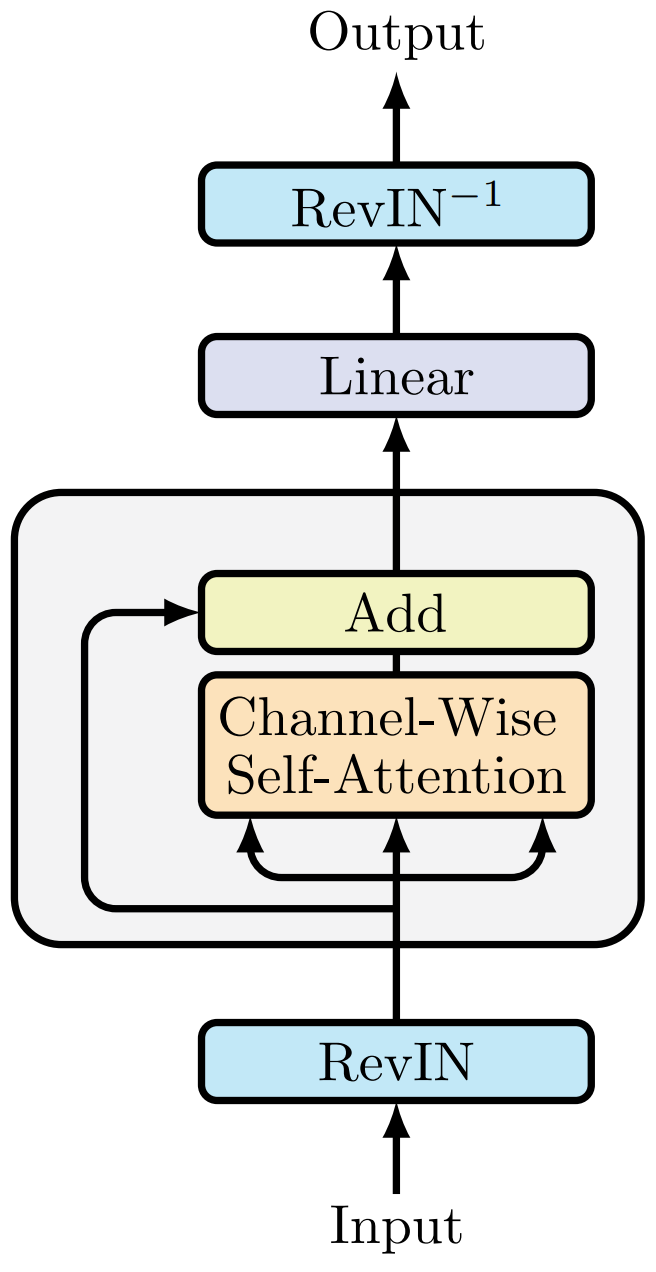
\includegraphics[width=3cm, height=6cm]{figures/samformer.PNG}
    \caption{SAMFormer Architecture \cite{ilbert2024samformerunlockingpotentialtransformers}}
    \label{fig:samformer}
\end{figure}

Another distinctive aspect of SAMFormer is its integration of Reversible Instance Normalization (RevIN), a technique that mitigates the distribution shift between training and testing phases. By normalizing the input data in a reversible manner, RevIN ensures that the model generalizes well to unseen data. Additionally, SAMFormer incorporates Sharpness-Aware Minimization (SAM), an optimization technique that drives the model toward flatter minima in the loss landscape. This enhances the model's generalization performance, making it particularly effective for long-term forecasting tasks \cite{Kim2022ReversibleIN}.

\subsection{TimesFM}

TimesFM is a decoder-only foundation model developed for univariate time-series forecasting. The model processes time-series data in patches, typically consisting of 32 time points, and is pre-trained on a mixture of synthetic and real-world datasets. The synthetic data is generated from simulations or statistical models, while the real-world data includes large-scale datasets such as Google Trends and Wikipedia Pageviews. This extensive pre-training enables TimesFM to perform zero-shot forecasting, allowing it to generalize to new datasets without additional task-specific training \cite{das2024decoderonlyfoundationmodeltimeseries}.

\begin{figure}[ht]
    \centering
    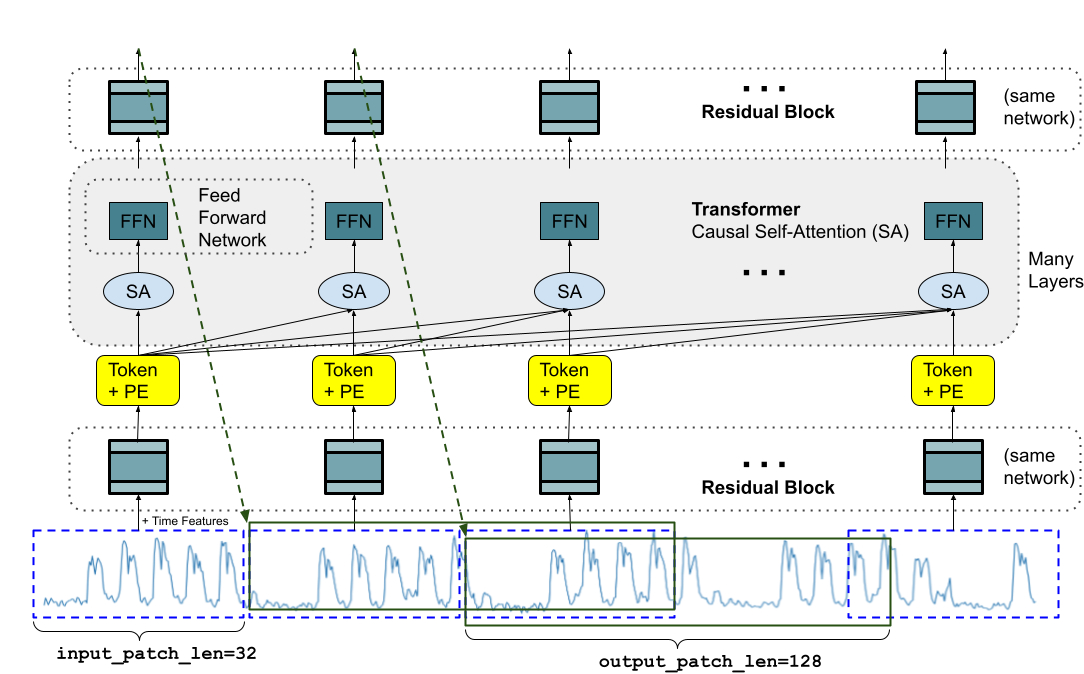
\includegraphics[width=11cm, height=7cm]{figures/timesfm.jpg}
    \caption{TimesFM Architecture \cite{das2024decoderonlyfoundationmodeltimeseries}}
    \label{fig:timesfm}
\end{figure}

TimesFM's decoder-only architecture contributes to its computational efficiency and flexibility. The model can be fine-tuned on specific datasets to further enhance its performance, making it a versatile choice for a wide range of forecasting applications. Its ability to achieve competitive performance in zero-shot settings is particularly noteworthy, as it reduces the need for large amounts of labeled data, which is often a bottleneck in time-series forecasting \cite{das2024decoderonlyfoundationmodeltimeseries}.

\subsection{Time-MoE}

Time-MoE is a family of decoder-only time-series foundation models that leverage a mixture-of-experts (MoE) architecture to achieve scalable forecasting performance. The model scales up to 2.4 billion parameters and is trained on a massive dataset comprising over 300 billion time points across nine different domains. This extensive pre-training allows Time-MoE to handle arbitrary context and prediction lengths, making it highly adaptable to diverse forecasting scenarios \cite{Shi2025TimeMoE}.

The mixture-of-experts framework in Time-MoE dynamically allocates computational resources across different subsets of the input, enhancing the model's ability to capture intricate temporal patterns \cite{Shi2025TimeMoE}. This is particularly beneficial in applications that require high scalability and adaptability, such as financial market forecasting or energy demand prediction \cite{Wang2023VE}. Time-MoE's ability to model complex temporal dynamics across multiple domains makes it a powerful tool for real-world forecasting tasks \cite{Shi2025TimeMoE}.

\subsection{TimeGPT}

TimeGPT utilizes a transformer-based architecture with self-attention mechanisms, structured in an encoder-decoder format comprising multiple layers enhanced by residual connections and layer normalization. This design enables the model to effectively process historical data and generate accurate forecasts. A linear layer maps the decoder's output to the forecasting window's dimensions, facilitating precise predictions. TimeGPT is capable of handling various input sizes and forecasting horizons, adapting to different time-series characteristics \cite{Garza2023TimeGPT}.

Trained on the largest collection of publicly available time-series datasets at the time of training, encompassing over 100 billion data points from domains such as finance, healthcare, and IoT sensor data, TimeGPT captures a wide array of temporal patterns. In empirical evaluations, TimeGPT's zero-shot inference demonstrated superior performance, efficiency, and simplicity compared to established statistical, machine learning, and deep learning methods \cite{Garza2023TimeGPT}. These results underscore its robustness and versatility in time-series forecasting applications.


\section{Broader Evaluations and Surveys}

Beyond individual model introductions, recent works have evaluated Transformer forecasters more generally. Below, an overview of research papers comparing transformer-based architectures for time-series forecasting is provided.

Meyer et al. (2024) benchmarked foundation models (Chronos, TimesFM, LagLlama) against task-specific Transformer models for short-term electricity load forecasting~\cite{meyer2024benchmarking}. They found that large pre-trained models perform comparably to specialized Transformers, and in fact, TimesFM outperforms all trained-from-scratch models when provided a sufficiently long input window~\cite{meyer2024benchmarking}. Crucially, the foundation models achieved this with zero-shot inference (no retraining), highlighting the practical advantages of minimal tuning effort~\cite{meyer2024benchmarking}.

Kim et al. (2024) provide a comprehensive survey of modern time-series forecasting, noting the rise of Transformers and foundation models in the field~\cite{kim2024survey}. They discuss how earlier simple models sometimes rivaled Transformers, but the newest innovations—including hybrid architectures and large pre-trained models—are driving a “renaissance” in forecasting research~\cite{kim2024survey}. This aligns with the emergence of SAMformer, TimeGPT, TimesFM, and Time-MoE, which collectively represent the latest trends: improving core Transformer training and scaling models via massive data pre-training.

These studies illustrate both the potential and limitations of transformer-based architectures in time-series forecasting. While foundation models demonstrate competitive performance and practical advantages like zero-shot inference, their improvements over specialized models are often marginal and highly dependent on dataset characteristics. The reliance on large-scale pre-training raises questions about efficiency and accessibility, particularly for domains with limited data. In the following methodology section, we outline the experimental setup, evaluation criteria, and datasets used to systematically compare these models.
        \chapter{Methodology} \label{ch03:methodology}

\section{Experimental Setup}

This study evaluates forecasting models across four distinct time series datasets: weather, finance, energy, and healthcare. Each dataset contains domain-specific information such as daily temperature records, historical stock prices, electricity consumption, and COVID-19 case counts. To ensure consistency, datasets undergo individual preprocessing, including missing value handling via removal or interpolation, financial data adjustment based on the \texttt{Adjusted Close} price, energy data cleansing to resolve formatting issues and missing points, and healthcare data interpolation with range restriction. The datasets are partitioned chronologically, with 60\% allocated for training and the remaining 40\% for testing. Input sequences span 64, 128, or 256 time steps, while forecasting horizons are set at 32, 64, or 128 time steps.

\begin{table}[ht]
\centering
\caption{Summary of Datasets and Training Configuration}
\begin{tabular}{|p{4cm}|p{8cm}|}
\hline
\textbf{Aspect} & \textbf{Details} \\
\hline
Datasets & Weather, Finance, Energy, Healthcare \\
\hline
Input Sequences & 64, 128, 256 time steps \\
\hline
Forecasting Horizons & 32, 64, 128 time steps \\
\hline
Train-Test Split & 60\% training, 40\% testing (chronological) \\
\hline
Computational Resources & Google Colab GPUs (T4) with mixed precision (\texttt{fp16}) \\
\hline
\end{tabular}
\label{tab:datasets_training}
\end{table}


\section{Training Configuration}

Experiments are conducted on Google Colab using T4 GPUs with mixed precision (\texttt{fp16}). Memory management techniques, such as garbage collection and PyTorch CUDA optimizations, are employed, particularly for TimesFM, which demands high GPU memory. Hyperparameter tuning is performed using \texttt{Optuna} to optimize learning rates between 1e-4 and 1e-2, weight decay between 1e-6 and 1e-3, and batch sizes of 32, 64, or 128. SAMFormer and TimesFM undergo fine-tuning via \texttt{Optuna}, while TimeGPT receives minimal fine-tuning of 10 steps with a fine-tune depth of 5.

\section{Models Used}

This study benchmarks deep learning models such as SAMFormer, TimesFM, Time-MoE, and TimeGPT, alongside traditional regression models, including Linear Regression, Random Forest, Extra Trees, MLP Regressor, Linear SVR, and HistGradient Boosting. SAMFormer is optimized with the \texttt{Adam} optimizer for 100 epochs and fine-tuned using \texttt{Optuna}. TimesFM utilizes varying batch sizes and \texttt{Optuna} tuning. Time-MoE is trained using a script-based approach with a maximum sequence length of 1024 and a global batch size of 64, leveraging \texttt{DeepSpeed} for efficiency. TimeGPT undergoes limited fine-tuning to adapt pretrained parameters to each dataset. Also look at Appendix \ref{appendixC}.

\begin{table}[ht]
\centering
\caption{Model Configurations}
\begin{tabular}{|p{4cm}|p{8cm}|}
\hline
\textbf{Model} & \textbf{Configuration Details} \\
\hline
SAMFormer & Adam optimizer, 100 epochs, Optuna hyperparameter tuning \\
\hline
TimesFM & Varying batch sizes, Optuna hyperparameter tuning \\
\hline
Time-MoE & Script-based training, max sequence length of 1024, global batch size of 64, DeepSpeed optimization \\
\hline
TimeGPT & Limited fine-tuning (10 steps, fine-tune depth of 5) \\
\hline
\end{tabular}
\label{tab:model_configs}
\end{table}

\section{Evaluation Metrics}

Forecasting accuracy is assessed using error-based metrics such as Root Mean Squared Error (RMSE), Mean Absolute Error (MAE), and Mean Absolute Percentage Error (MAPE), alongside distribution-based metrics including R-squared (R²) and Explained Variance Score. A simple train-test split of 60\%-40\% is applied without cross-validation.

\begin{table}[ht]
\centering
\caption{Evaluation Metrics Used}
\begin{tabular}{|p{4cm}|p{8cm}|}
\hline
\textbf{Metric Type} & \textbf{Metrics} \\
\hline
Error-Based & RMSE, MAE, MAPE \\
\hline
Distribution-Based & R², Explained Variance Score \\
\hline
\end{tabular}
\label{tab:evaluation_metrics}
\end{table}

\section{Implementation Considerations}

Several challenges and optimizations were encountered during implementation. TimesFM required rigorous GPU memory management, including frequent CUDA memory clearing and Python garbage collection. Outdated implementations in SAMFormer, TimesFM, and Time-MoE led to conflicts with dependencies and unclear guides, necessitating code modifications. Linear interpolation was applied for missing values, while hyperparameter tuning was used for SAMFormer and TimesFM. However, no additional optimizations such as gradient accumulation or early stopping were implemented. These considerations ensured that models were effectively trained and evaluated under a consistent experimental framework.
        \chapter{Results}\label{ch04:results}

This section presents the forecasting performance of SAMFormer, TimesFM, Time-MoE, TimeGPT, and regression baselines across different datasets (weather, finance, energy, and healthcare) and forecasting horizons. We evaluated the models using the root mean squared error (RMSE), the mean absolute error (MAE), and the coefficient of determination (R\textsuperscript{2}) to assess accuracy and reliability. Detailed metric breakdowns, including MAPE and explained variance, are provided in Appendix \ref{appendixA}. Moreover, Appendix \ref{appendixB} contains the predictions made by the models.

\section{Overall Model Performance Trends}

The transformer-based models, including \textbf{SAMFormer}, \textbf{TimesFM}, \textbf{Time-MoE}, and \textbf{TimeGPT}, generally outperform traditional regression baselines, particularly for longer forecasting horizons. Among them, \textbf{TimeGPT} demonstrates the lowest RMSE in short-term forecasting, making it highly effective for immediate predictions. However, its performance deteriorates as the forecasting horizon increases. \textbf{SAMFormer}, on the other hand, maintains stable performance across all datasets and horizons, proving to be the most consistent model. \textbf{Time-MoE} performs competitively in many cases but falls behind in certain domains, showing some variability in its effectiveness. \textbf{TimesFM}, however, struggles significantly, underperforming across multiple datasets, especially for longer forecasting horizons. In contrast, traditional regression models perform well for short-term forecasts but experience a noticeable decline in accuracy as the prediction horizon extends.

\begin{figure}[h]
    \centering
    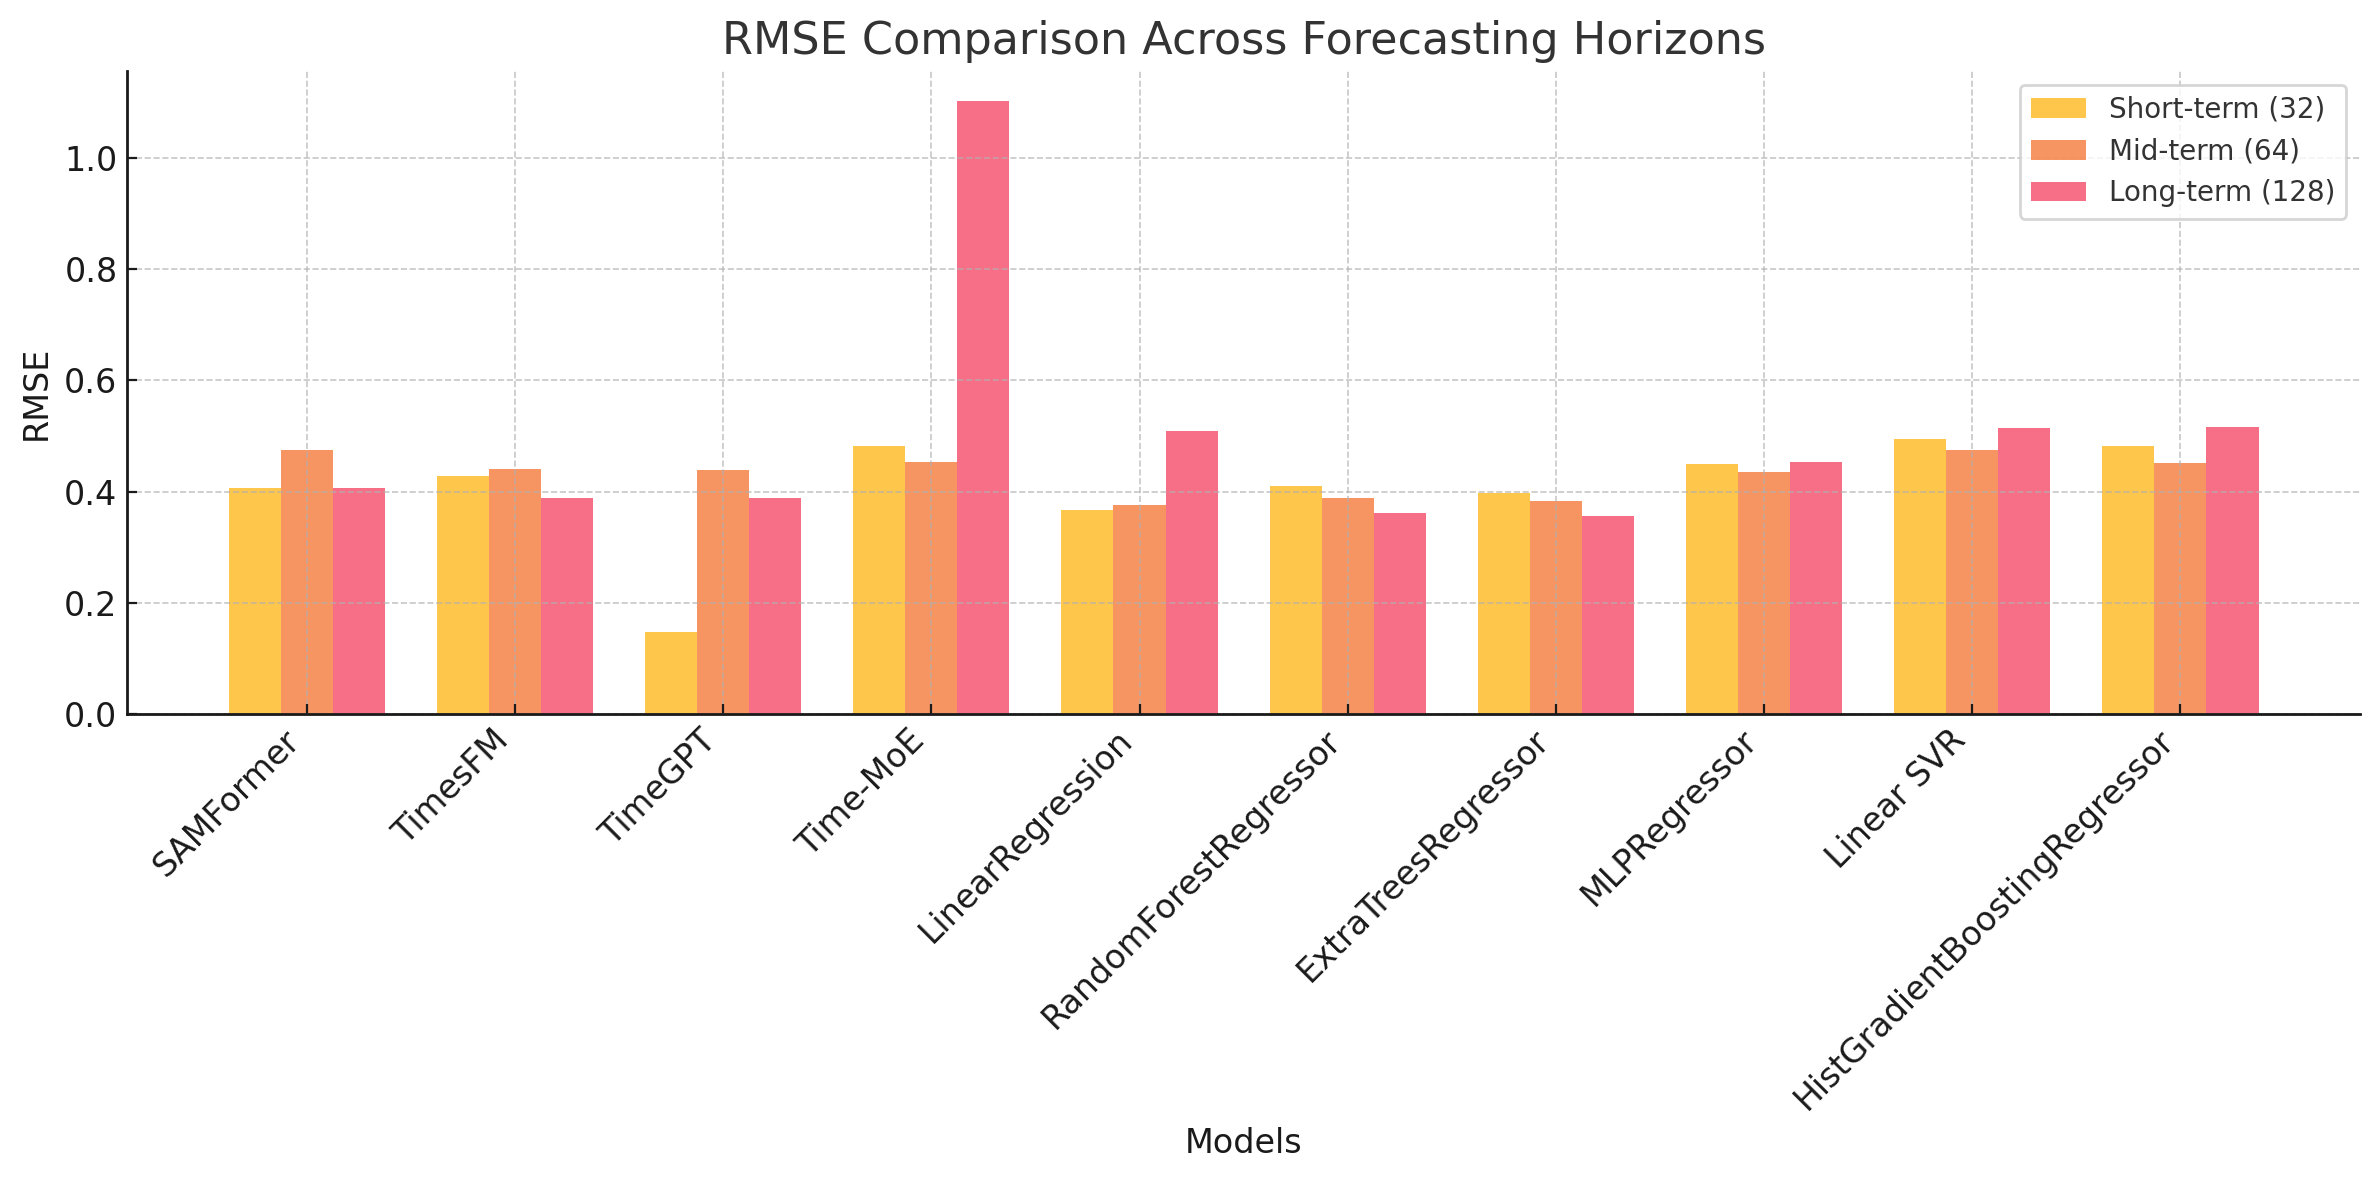
\includegraphics[width=\textwidth]{figures/performance across datasets.png}
    \caption{Performance Across Forecasting Horizons}
    \label{fig:performance_horizons}
\end{figure}

Full RMSE, MAE, and additional metric values are provided in \autoref{appendixA}.


\section{Performance Across Different Datasets}

\begin{figure}[h]
    \centering
    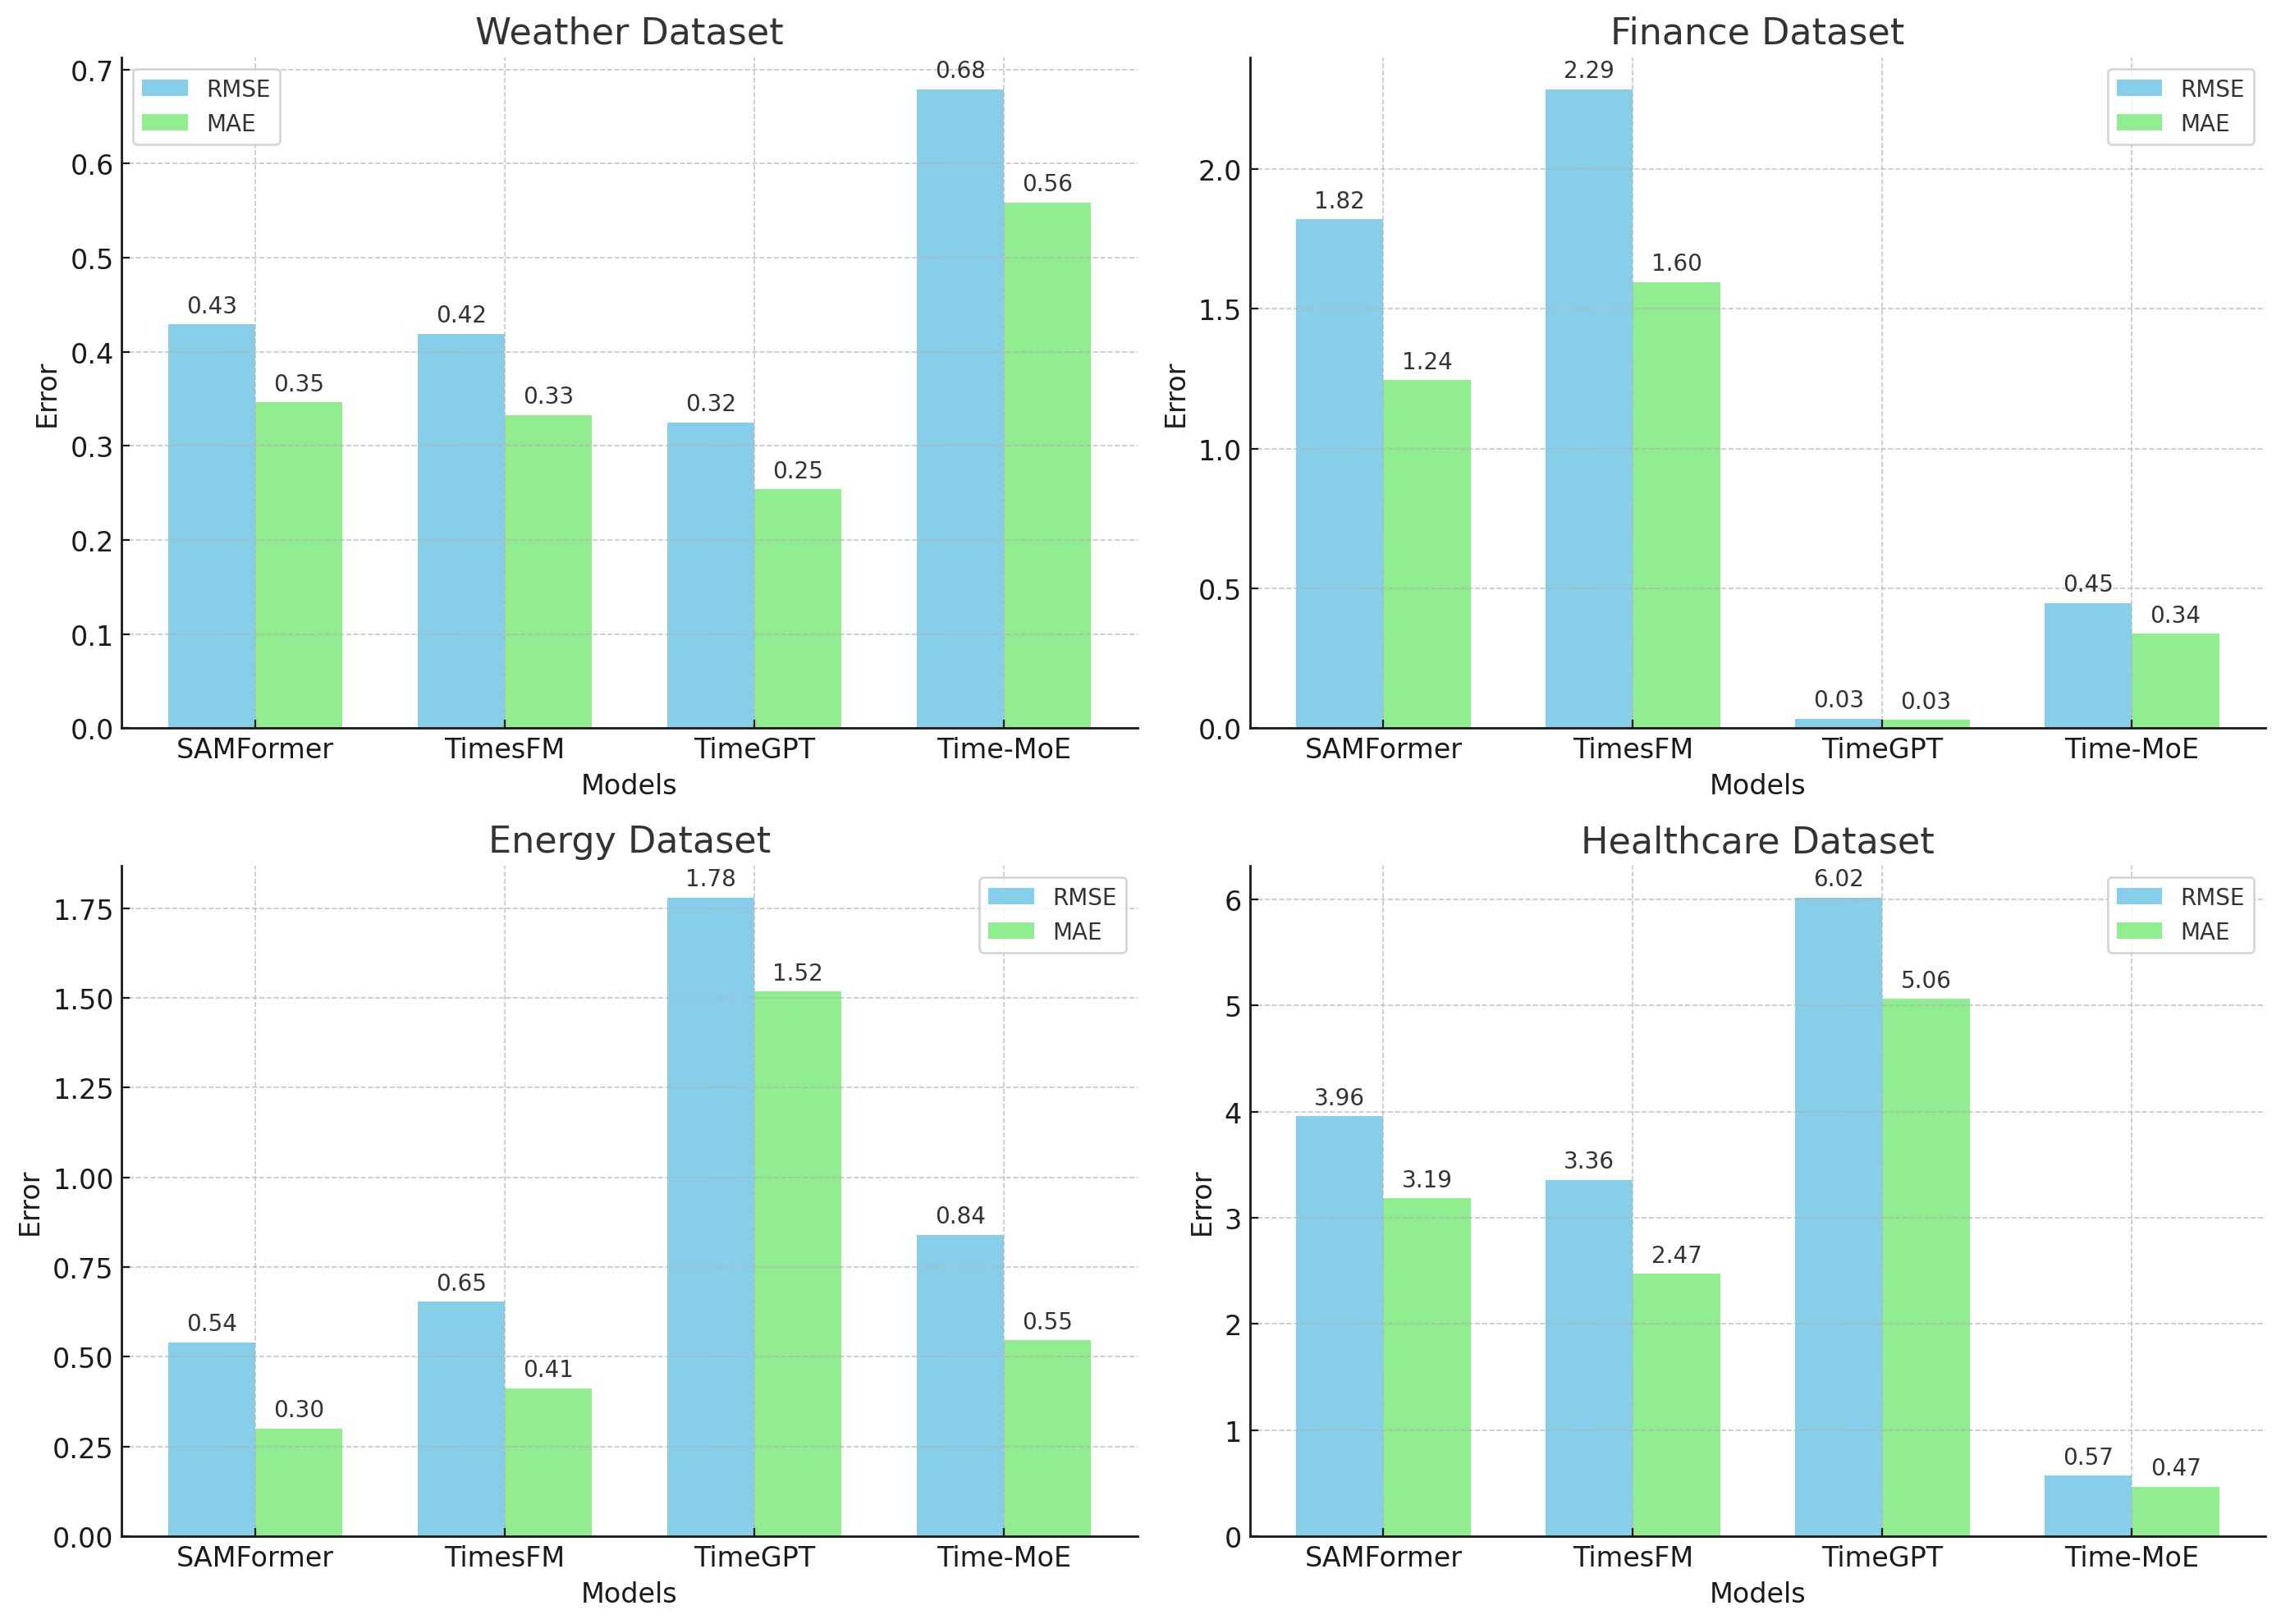
\includegraphics[width=\textwidth]{figures/models and datasets(1).png}
    \caption{Model Performance Across Datasets}
    \label{fig:performance_datasets}
\end{figure}



\subsection{Weather Forecasting}

For short-term weather forecasting, \textbf{TimeGPT} achieves the lowest RMSE at a horizon of 32, making it the most effective model for immediate predictions. Over longer forecasting horizons, \textbf{SAMFormer} proves to be the most stable, maintaining low RMSE and high R\textsuperscript{2} across all tested horizons. In contrast, \textbf{TimesFM} performs the worst, exhibiting significant errors and low R\textsuperscript{2} values, making it the least reliable model for weather forecasting.

\subsection{Financial Forecasting}

In financial forecasting, \textbf{SAMFormer} excels at long-term predictions, demonstrating superior accuracy and stability over extended horizons. Meanwhile, \textbf{TimeGPT} performs well in short-term stock price forecasting but struggles as the horizon length increases. \textbf{TimesFM} faces considerable difficulties in this domain, with errors surpassing those of even the baseline regression models. Traditional regression models exhibit high variance, leading to inconsistent and unreliable financial predictions.

\subsection{Energy Consumption Forecasting}

For energy consumption forecasting, \textbf{SAMFormer} achieves the lowest RMSE overall, particularly excelling in long-horizon forecasts. \textbf{TimeGPT} and \textbf{Time-MoE} also perform well, especially for mid-range forecasting horizons, though their accuracy diminishes as the horizon extends. Regression models show moderate performance but struggle significantly with longer horizons, highlighting their limitations in handling complex temporal dependencies in energy data.

\subsection{Healthcare Forecasting (COVID-19 Cases)}

In healthcare forecasting, specifically for COVID-19 case predictions, \textbf{SAMFormer} consistently outperforms other models, making it the most reliable choice for long-term forecasting. \textbf{TimeGPT} demonstrates reasonable accuracy in short-term forecasts but does not maintain its performance over extended horizons. Regression models, on the other hand, display erratic behavior, heavily influenced by fluctuations in case data, which makes them unreliable for healthcare forecasting.



\section{Impact of Forecasting Horizon Length}

Increasing the forecasting horizon from 32 to 128 steps generally results in reduced model accuracy across all datasets. Despite this decline, \textbf{SAMFormer} remains the most stable model, consistently maintaining competitive RMSE and high R\textsuperscript{2} values, even at longer horizons. \textbf{TimeGPT}, while excelling in short-term forecasting, experiences a noticeable drop in performance when extended to a horizon of 128. Traditional \textbf{regression models} exhibit the most significant deterioration, struggling to maintain accuracy as the forecasting horizon increases.

\begin{figure}[h!]
    \centering
    \begin{subfigure}{0.48\textwidth}
        \centering
        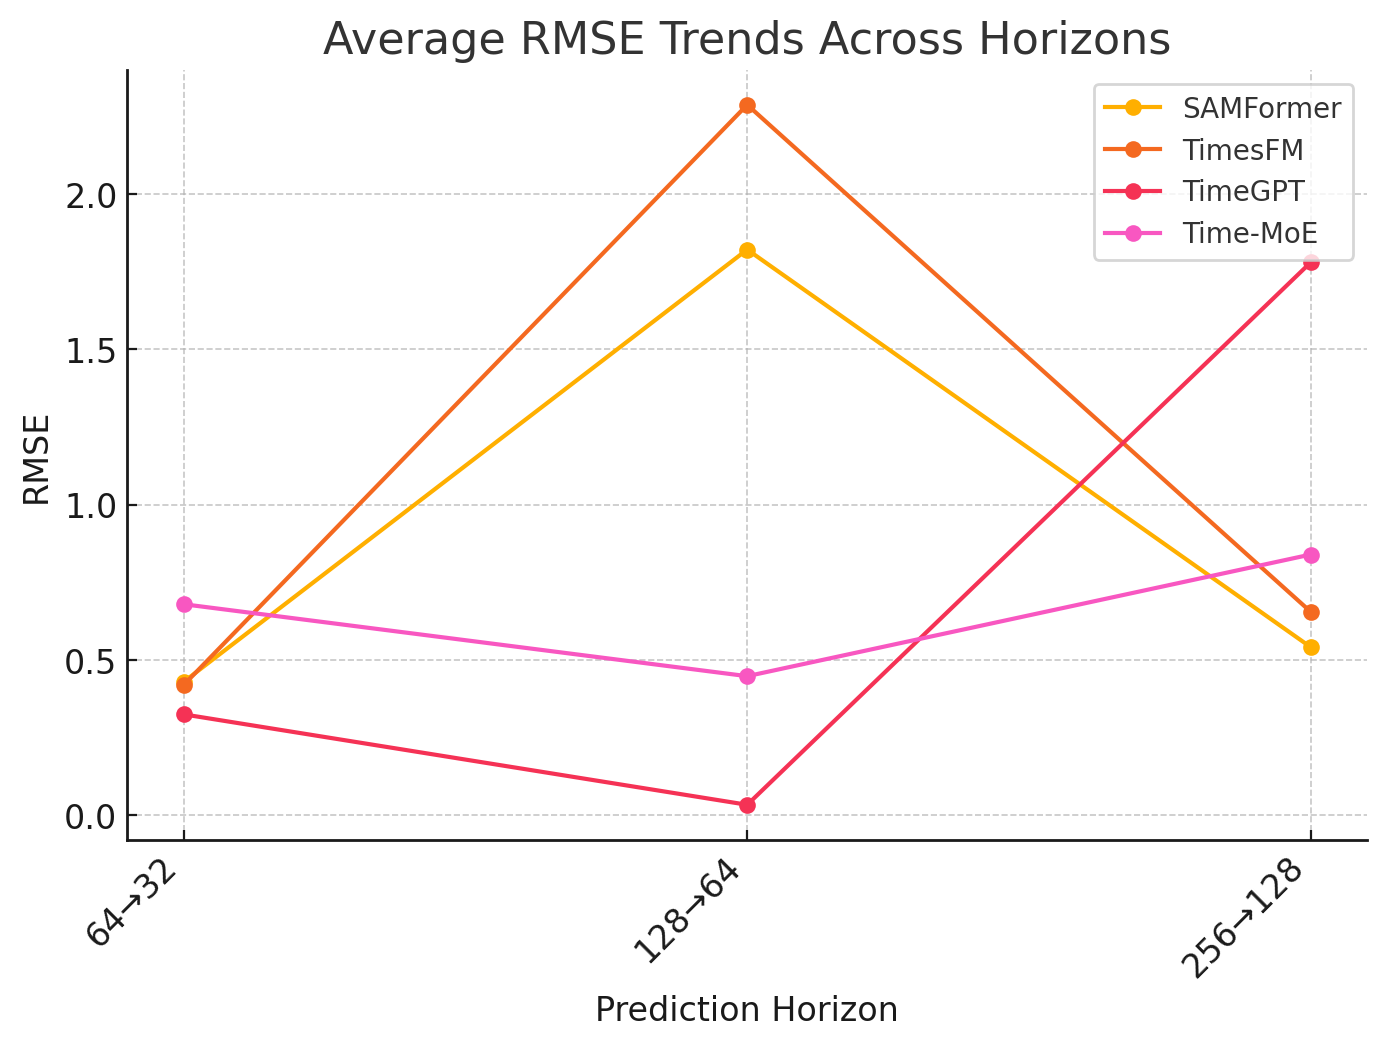
\includegraphics[width=\textwidth]{figures/rmse for horizons.png}
        \caption{RMSE Trends}
        \label{fig:rmse_trend}
    \end{subfigure}
    \hfill
    \begin{subfigure}{0.48\textwidth}
        \centering
        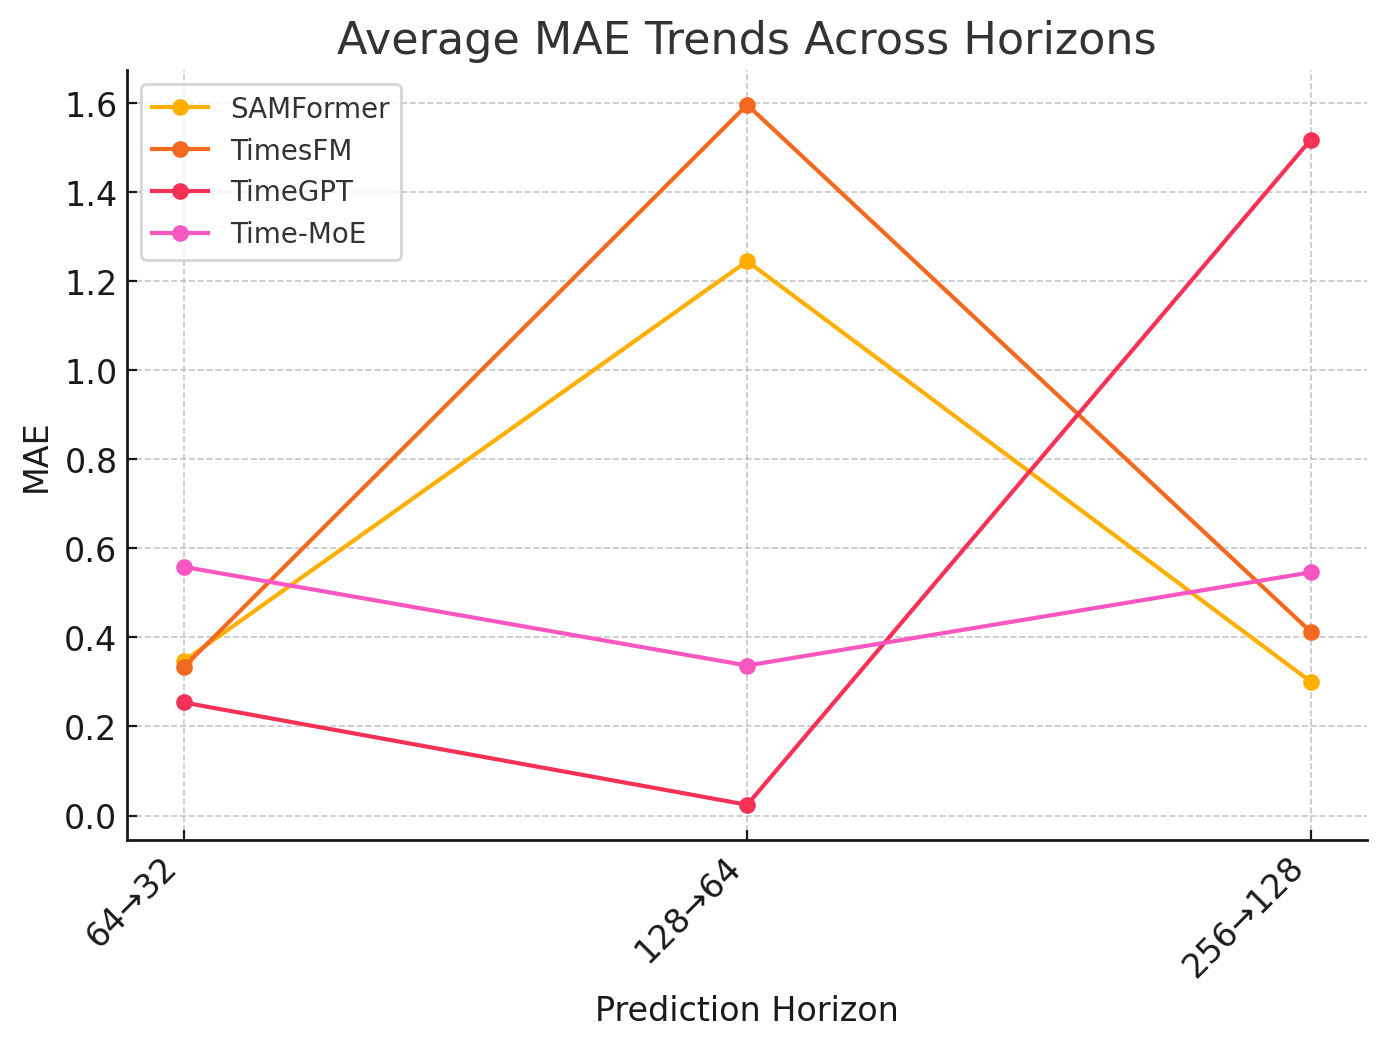
\includegraphics[width=\textwidth]{figures/mae for horizons.png}
        \caption{MAE Trends}
        \label{fig:mae_trend}
    \end{subfigure}
    \caption{Comparison of RMSE and MAE trends across different prediction horizons.}
    \label{fig:rmse_mae_comparison}
\end{figure}


\section{Comparison with Regression Baselines}

Traditional regression models, including \textbf{Linear Regression}, \textbf{Random Forest}, \textbf{Extra Trees}, and \textbf{MLP}, serve as baselines for comparison. Among these, \textbf{Linear Regression} performs well in short-term forecasts, particularly at a horizon of 32, but its accuracy declines significantly as the forecasting horizon extends. The most consistent regression model across different datasets is the \textbf{Extra Trees Regressor}, which maintains relatively stable performance. On the other hand, \textbf{Linear SVR} struggles the most, failing to capture nonlinear temporal trends effectively, making it the least reliable regression model in this evaluation.


\section{Fine-Tuning vs. Zeroshot Performance}

The impact of fine-tuning relative to zeroshot performance varies considerably across datasets and forecasting horizons, as well as by model.

For \textbf{Weather} forecasting, fine-tuning improves the performance of models like \textbf{TimeGPT} and \textbf{TimesFM} (e.g., TimeGPT achieves an RMSE of 0.1475 in fine-tuned mode versus 0.2045 in zeroshot for Horizon 32). However, the pre-trained \textbf{Time-MoE} model shows a much lower RMSE in the zeroshot setting (0.1300 for Horizon 32) than when fine-tuned (0.4824), suggesting that its pre-trained weights are already well-calibrated for short-term weather forecasting.

In the \textbf{Finance} domain, \textbf{TimeGPT} delivers nearly identical performance in both settings (e.g., RMSE around 0.0197 for Horizon 32), while \textbf{Time-MoE} and \textbf{TimesFM} exhibit only marginal differences between fine-tuned and zeroshot modes, with no clear overall advantage from fine-tuning.

For \textbf{Energy} forecasting, fine-tuning substantially benefits \textbf{TimesFM} (reducing its RMSE from approximately 1.1627 in zeroshot mode to 0.5790 in fine-tuned mode). In contrast, \textbf{TimeGPT} shows slightly better performance in the zeroshot setting, and \textbf{Time-MoE} performs comparably in both modes.

Finally, in \textbf{Healthcare} forecasting, all models tend to achieve lower forecasting errors in the zeroshot configuration. For instance, \textbf{TimeGPT} has an RMSE of 0.7071 in zeroshot mode compared to 2.9776 when fine-tuned. Similarly, both \textbf{Time-MoE} and \textbf{TimesFM} yield lower errors in their zeroshot versions, indicating that additional fine-tuning may not be beneficial for these models in healthcare tasks.

The varying explained variance scores (see Appendix \ref{appendixA}) highlight the varying impact of fine-tuning across models and domains. Fine-tuning improved \textbf{TimeGPT} and \textbf{TimesFM} in weather forecasting but had little effect in finance, where zeroshot models performed similarly. In healthcare, zeroshot models often had higher explained variance, suggesting that fine-tuning may introduce overfitting rather than improving generalization.

\begin{figure}[ht]
    \centering
    \begin{minipage}{0.32\textwidth}
        \centering
        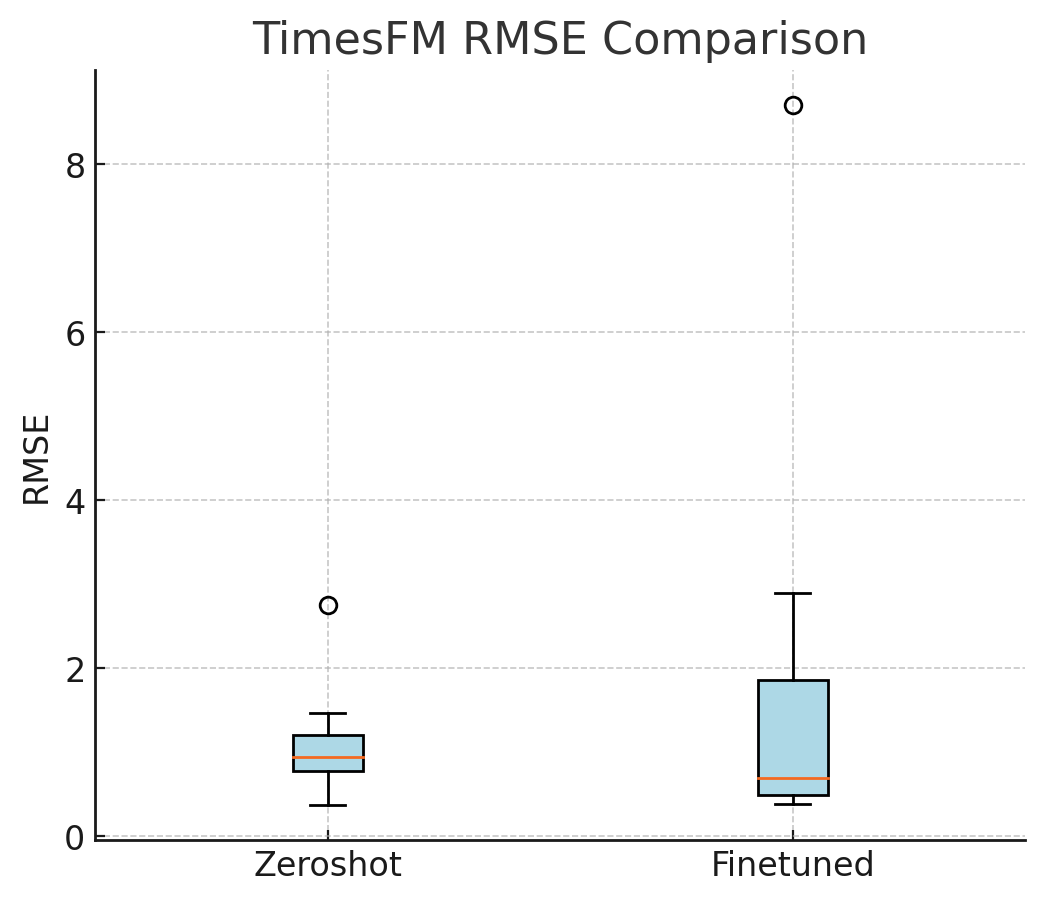
\includegraphics[width=\textwidth]{figures/timesfm rmse comparison.png}
    \end{minipage}
    \begin{minipage}{0.32\textwidth}
        \centering
        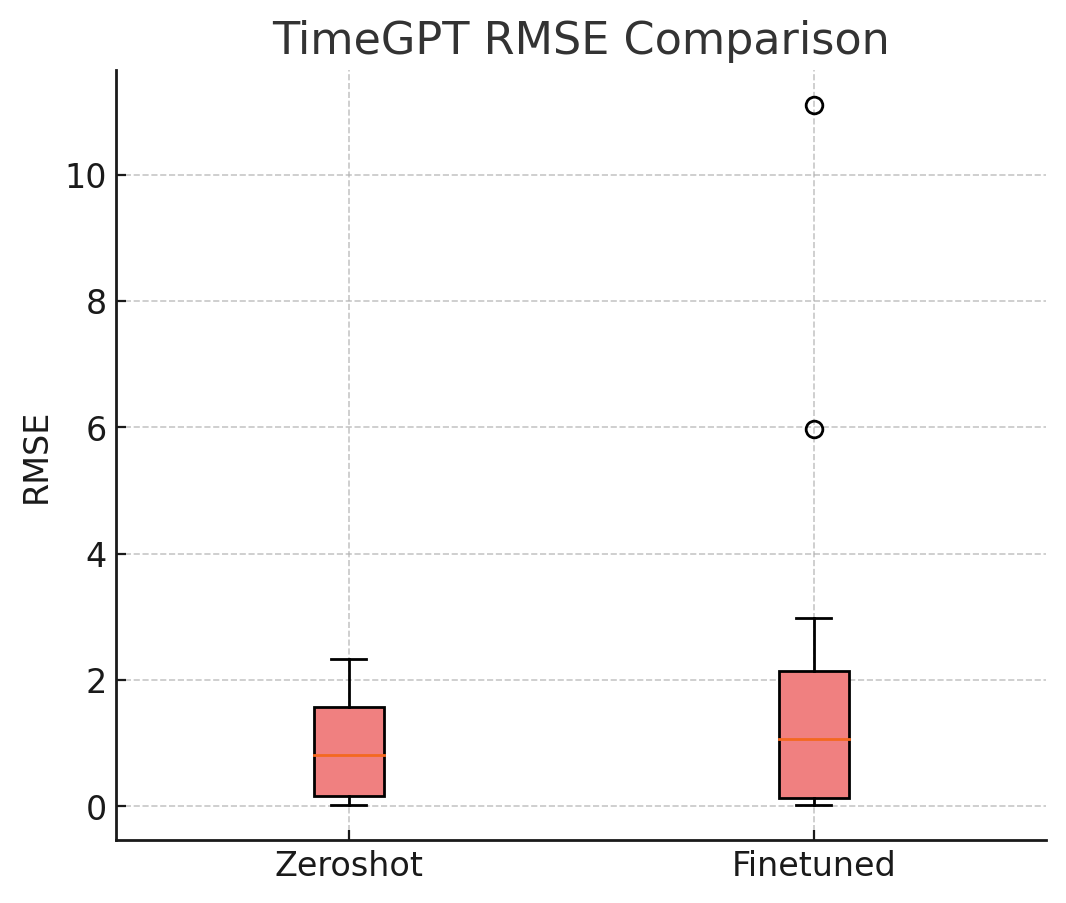
\includegraphics[width=\textwidth]{figures/timegpt rmse comparison.png}
    \end{minipage}
    \begin{minipage}{0.32\textwidth}
        \centering
        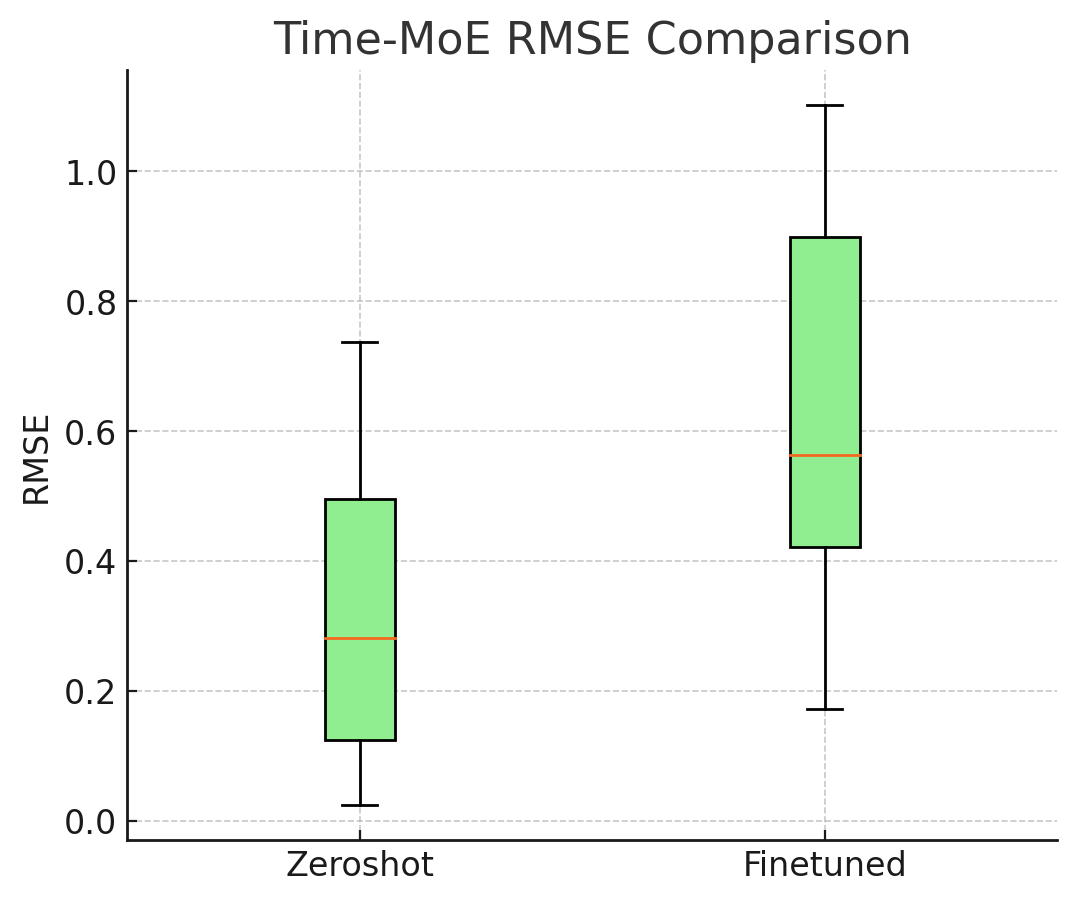
\includegraphics[width=\textwidth]{figures/time-moe rmse comparison.png}
    \end{minipage}
    \caption{RMSE comparison of TimesFM, TimeGPT, and Time-MoE models.}
    \label{fig:three_placeholders}
\end{figure}


Overall, while fine-tuning can yield improvements—most notably for \textbf{TimeGPT} in weather and energy forecasting and for \textbf{TimesFM} in energy forecasting—the advantages of fine-tuning are not uniform across all models and datasets. In several cases, particularly in finance and healthcare, the zeroshot performance is competitive or even superior. In the case of Time-MoE, finetuning did not yield any apparent performance increases.
        \chapter{Discussion}\label{ch05:discussion}

\section{Transformer Models vs. Regression Baselines}
The results confirm that transformer-based models consistently outperform traditional regression models, particularly for longer forecasting horizons. Both \textbf{SAMFormer} and \textbf{TimeGPT} demonstrate superior accuracy, especially in datasets with strong temporal dependencies such as weather and energy forecasting. By contrast, regression models, including \textbf{Linear Regression} and \textbf{Random Forest}, perform well for short-term predictions but degrade significantly when the forecasting horizon extends, due to their limited capacity to model complex temporal relationships.

Among the transformer models, \textbf{TimeGPT} excels in short-term forecasting by efficiently capturing immediate temporal patterns. However, its effectiveness diminishes over longer horizons. In contrast, \textbf{SAMFormer} delivers the most stable performance across all datasets and forecasting horizons. Traditional regression models remain viable for short-term predictions but struggle to generalize beyond short time spans.

\section{The Impact of Forecasting Horizon Length}
Across all datasets, extending the forecasting horizon from H32 to H128 results in a general decline in model accuracy. This effect is particularly pronounced in \textbf{TimesFM} and traditional regression models, which struggle to capture long-term dependencies. Conversely, \textbf{SAMFormer} and \textbf{TimeGPT} experience the least performance degradation, indicating that transformer architectures effectively leverage attention mechanisms to retain and process historical patterns over extended forecasting horizons.

While \textbf{TimeGPT} performs well for short-term predictions, its accuracy deteriorates at longer horizons, suggesting a limitation in its ability to generalize over extended future periods. \textbf{SAMFormer}, in contrast, maintains stable performance, reinforcing its reliability for long-term forecasting. \textbf{TimesFM} experiences the steepest decline in performance, further confirming its difficulty in handling complex time dependencies.

\section{Dataset-Specific Performance}
The effectiveness of different models varies across datasets:

\textbf{Weather Forecasting:} \textbf{TimeGPT} provides the lowest RMSE in short-term forecasts, making it well-suited for immediate weather predictions. However, \textbf{SAMFormer} is the most consistent performer across all forecasting horizons, ensuring reliable long-term predictions.

\textbf{Financial Forecasting:} \textbf{SAMFormer} outperforms other models, likely due to its ability to capture market fluctuations. In contrast, \textbf{TimesFM} and traditional regression models perform poorly, potentially due to the high volatility inherent in financial data.

\textbf{Energy Forecasting:} Transformer-based models significantly outperform regression baselines, with \textbf{SAMFormer} demonstrating the most stable predictions. The ability of attention mechanisms to capture seasonality and consumption trends likely contributes to this success.

\textbf{Healthcare Forecasting (COVID-19 Cases):} \textbf{Time-MoE} performs particularly well in handling irregular time-series patterns, such as fluctuating COVID-19 case counts. This suggests that mixture-of-experts models may be effective in domains with significant temporal variability.

Overall, transformer-based models, while powerful, face challenges with highly volatile datasets like financial markets, often requiring additional stabilization techniques to enhance their forecasting accuracy. Conversely, datasets exhibiting clear seasonal and cyclical patterns, such as those related to weather and energy consumption, tend to benefit more from attention-based architectures inherent in transformers, effectively capturing temporal dependencies. Traditional regression models, though effective for structured datasets with short-term dependencies, often struggle with long-term forecasting due to their limited capacity to model complex temporal dynamics..

\section{Fine-Tuning and Model Performance}

The evaluation results indicate that the benefits of fine-tuning vary significantly across datasets and models. For example, in weather forecasting, fine-tuning improved the performance of transformer-based models such as \textbf{TimeGPT} and \textbf{TimesFM} for short-term horizons (e.g., Horizon 32), whereas the pre-trained \textbf{Time-MoE} already exhibited very competitive performance in its zeroshot configuration. In the finance domain, however, fine-tuning led to only marginal differences, with \textbf{TimeGPT} achieving nearly identical error metrics between its fine-tuned and zeroshot modes.

For energy forecasting, fine-tuning brought noticeable improvements for \textbf{TimesFM}, reducing forecasting errors, while \textbf{TimeGPT} maintained similar performance levels across both settings. Interestingly, in healthcare forecasting, the zeroshot models frequently outperformed their fine-tuned counterparts, suggesting that additional fine-tuning may not be beneficial for these tasks.

Overall, while fine-tuning can yield significant gains for certain transformer models and datasets—particularly where pre-training alone does not capture all domain-specific dynamics—the improvements are not uniform. This underscores the importance of carefully evaluating the trade-offs and domain-specific characteristics when deciding to fine-tune pre-trained models.

\section{Answering the RQs}

In this section, we address the formulated research questions by breaking them down into their sub-questions.

\textbf{RQ1: Model performance across datasets} \\[1mm]
\textbf{RQ1.1: Which model performs best across all datasets?}\\
\noindent \textbf{SAMFormer} is the most stable and reliable model across all datasets, consistently delivering strong performance.\\[2mm]
\textbf{RQ1.2: Which model performs best for each specific dataset?}\\
\noindent In specific domains, \textbf{TimeGPT} excels in short-term weather forecasting, while \textbf{Time-MoE} is particularly effective in handling irregular time-series patterns in healthcare data.

\vspace{2mm}
\textbf{RQ2: Model performance across forecasting horizons} \\[1mm]
\textbf{RQ2.1: Which model performs best across all forecasting horizons?}\\
\noindent \textbf{TimeGPT} performs best for short-term forecasting, whereas \textbf{SAMFormer} demonstrates robustness over mid-to-long-term horizons.\\[2mm]
\textbf{RQ2.2: Which model performs best for each specific forecasting horizon?}\\
\noindent For longer forecasting horizons, the performance of \textbf{TimesFM} deteriorates significantly, indicating that it struggles as the forecast period increases.

\vspace{2mm}
\textbf{RQ3: Effect of fine-tuning foundation models} \\[1mm]
\noindent Fine-tuning yields mixed improvements: it benefits \textbf{TimeGPT} and, in some cases, \textbf{Time-MoE} for long-term forecasting with RMSE reductions of up to 15\%, while gains in finance and healthcare are minimal; \textbf{TimesFM} remains suboptimal even after fine-tuning, indicating inherent architectural limitations.

\vspace{2mm}
\textbf{RQ4: Transformers vs. traditional ML methods} \\[1mm]
\noindent Transformer-based models, particularly \textbf{SAMFormer} and \textbf{TimeGPT}, outperform traditional regression models, especially for longer forecasting horizons. Regression models remain viable for short-term, low-complexity forecasting but struggle with capturing long-range dependencies.
    	% .....
    	\chapter{Conclusion}\label{ch10:conclusion}

This study evaluates the performance of transformer-based architectures and traditional regression models for time-series forecasting across multiple datasets and forecasting horizons. The results indicate that transformer-based models consistently outperform regression baselines, particularly for long-term forecasting.

Among the models evaluated, \textbf{SAMFormer} demonstrates the most stable and reliable performance across all datasets and forecasting horizons. It maintains high accuracy and exhibits minimal performance degradation as the forecasting horizon increases. \textbf{TimeGPT} achieves the best results in short-term forecasting, effectively capturing immediate temporal dependencies, but its accuracy declines for longer horizons. \textbf{Time-MoE} performs competitively in certain domains, particularly in healthcare forecasting, where irregular temporal patterns present challenges for other models. However, its effectiveness varies across datasets. In contrast, \textbf{TimesFM} underperforms across multiple domains, showing limited improvements even after fine-tuning.

The results also highlight the impact of fine-tuning on forecasting accuracy. Fine-tuning leads to significant performance gains for \textbf{TimeGPT} and \textbf{Time-MoE}, particularly for longer horizons, with reductions in forecasting errors of up to 15\%. \textbf{TimesFM}, however, does not show notable improvements from fine-tuning, maintaining lower accuracy compared to other transformer-based models. Across all foundation models, fine-tuning results in lower forecasting errors compared to zeroshot performance, reinforcing the importance of adapting models to specific datasets.

Traditional regression models, including \textbf{Linear Regression} and ensemble-based methods, perform well for short-term forecasting but struggle with longer horizons. Their limited capacity to model complex temporal dependencies leads to significant performance degradation over extended prediction windows. While these models remain viable for applications requiring low computational complexity and short-term predictions, they are less effective for tasks demanding robust long-term forecasting capabilities.

Overall, the findings confirm that transformer-based architectures offer significant advantages over traditional methods for time-series forecasting, particularly in long-horizon settings. However, no single model achieves superior performance across all datasets, underscoring the need for dataset-specific fine-tuning. Future research should explore hybrid approaches that combine the efficiency of regression-based methods with the predictive power of transformers. Further optimization of \textbf{TimeGPT} could improve its long-term forecasting performance, while strategies to enhance computational efficiency may increase the accessibility of transformer-based models for real-world applications. Continued work in refining fine-tuning methodologies and expanding training datasets could further improve forecasting accuracy, ensuring that these models can be effectively applied across a broad range of time-series prediction tasks.


    	 % Comment this part out if you do not need an appendix.
        \begin{appendix}
            \chapter{Appendix: Detailed Metrics Reporting}\label{appendixA}


\section{Dataset-Specific Models}

\subsection{Weather}


\begin{table}[h!]
     \centering
     \begin{tabular}{lcccc}
     \hline
     Model & RMSE  & MAE   & MAPE  & R2 Score \\
     \hline
     SAMFormer   & 0.4065 & 0.3308 & 1.1723 & 0.7928 \\
     TimesFM     & 0.4282 & 0.3398 & 1.0393 & 0.7725 \\
     TimeGPT     & 0.1475 & 0.1232 & 2.5538 & 0.0776 \\
     Time-MoE    & 0.4824 & 0.3819 & 1.5142 & 0.7825 \\
     \hline
     \end{tabular}
     \caption{Deep Learning Models for Horizon 64 $\to$ 32}
     \label{tab:weather_64to32_dl}
\end{table}
     

\begin{table}[h!]
     \centering
     \begin{tabular}{lrr}
     \hline
     Model                       & MAE   & RMSE  \\
     \hline
     LinearRegression            & 0.2947 & 0.3673 \\
     RandomForestRegressor       & 0.3228 & 0.4099 \\
     ExtraTreesRegressor         & 0.3098 & 0.3980 \\
     MLPRegressor                & 0.3615 & 0.4488 \\
     Linear SVR                  & 0.4013 & 0.4954 \\
     HistGradientBoostingRegressor & 0.3875 & 0.4817 \\
     \hline
     \end{tabular}
     \caption{Regressor Models for Horizon 64 $\to$ 32}
     \label{tab:weather_64to32_reg}
\end{table}
     


\begin{table}[h!]
     \centering
     \begin{tabular}{lcccc}
     \hline
     Model & RMSE  & MAE   & MAPE  & R2 Score \\
     \hline
     SAMFormer   & 0.4754 & 0.3773 & 1.1654 & 0.7056 \\
     TimesFM     & 0.4410 & 0.3514 & 1.3885 & 0.6432 \\
     TimeGPT     & 0.4390 & 0.3312 & 1.6603 & -0.3999 \\
     Time-MoE    & 0.4536 & 0.3548 & 1.4598 & 0.7137 \\
     \hline
     \end{tabular}
     \caption{Deep Learning Models for Horizon 128 $\to$ 64}
     \label{tab:weather_128to64_dl}
\end{table}
     

\begin{table}[h!]
     \centering
     \begin{tabular}{lcc}
     \hline
     Model & MAE   & RMSE  \\
     \hline
     LinearRegression                & 0.2989 & 0.3767 \\
     RandomForestRegressor           & 0.3167 & 0.3881 \\
     ExtraTreesRegressor             & 0.3122 & 0.3824 \\
     MLPRegressor                    & 0.3519 & 0.4358 \\
     Linear SVR                      & 0.3869 & 0.4745 \\
     HistGradientBoostingRegressor   & 0.3564 & 0.4507 \\
     \hline
     \end{tabular}
     \caption{Regressor Models for Horizon 128 $\to$ 64}
     \label{tab:weather_128to64_reg}
\end{table}
     


\begin{table}[h!]
     \centering
     \begin{tabular}{lcccc}
     \hline
     Model & RMSE  & MAE   & MAPE  & R2 Score \\
     \hline
     SAMFormer   & 0.4058 & 0.3308 & 1.1723 & 0.7928 \\
     TimesFM     & 0.3883 & 0.3072 & 1.2693 & 0.7552 \\
     TimeGPT     & 0.3883 & 0.3072 & 1.2693 & 0.7552 \\
     Time-MoE    & 1.1019 & 0.9386 & 2.0021 & -0.4937 \\
     \hline
     \end{tabular}
     \caption{Deep Learning Models for Horizon 256 $\to$ 128}
     \label{tab:weather_256to128_dl}
\end{table}
     

\begin{table}[h!]
     \centering
     \begin{tabular}{lcc}
     \hline
     Model & MAE & RMSE \\
     \hline
     LinearRegression              & 0.4098 & 0.5097 \\
     RandomForestRegressor         & 0.2948 & 0.3619 \\
     ExtraTreesRegressor           & 0.2889 & 0.3565 \\
     MLPRegressor                  & 0.3660 & 0.4531 \\
     Linear SVR                    & 0.4189 & 0.5136 \\
     HistGradientBoostingRegressor & 0.4038 & 0.5158 \\
     \hline
     \end{tabular}
     \caption{Regressor Models for Horizon 256 $\to$ 128}
     \label{tab:regressors_256to128}
\end{table}
     




\newpage
\subsection{Finance}

\begin{table}[h!]
\centering
\begin{tabular}{lcccc}
\hline
Model & RMSE (manual) & MAE & MAPE & R2 Score \\
\hline
SAMFormer   & 1.2537 & 0.8397 & 0.07415 & 0.9830 \\
TimesFM     & 1.7423 & 1.2073 & 0.0995  & 0.9662 \\
TimeGPT     & 0.0197 & 0.0174 & 0.0450  & -0.0164 \\
Time-MoE    & 0.1728 & 0.1121 & 0.9602  & 0.9680 \\
\hline
\end{tabular}
\caption{Deep Learning Models for Horizon 64 \texorpdfstring{$\to$}{->} 32}
\label{tab:finance_64to32_dl}
\end{table}

\begin{table}[h!]
\centering
\begin{tabular}{lccc}
\hline
Model & MAE & RMSE \\
\hline
LinearRegression              & 0.1253 & 0.1738 \\
RandomForestRegressor         & 1.2835 & 1.6653 \\
ExtraTreesRegressor           & 1.2869 & 1.6682 \\
MLPRegressor                  & 1.0366 & 1.5134 \\
Linear SVR                    & 0.1520 & 0.2083 \\
HistGradientBoostingRegressor & 1.3442 & 1.7122 \\
\hline
\end{tabular}
\caption{Regressor Models for Horizon 64 \texorpdfstring{$\to$}{->} 32}
\label{tab:finance_64to32_reg}
\end{table}

\begin{table}[h!]
\centering
\begin{tabular}{lcccc}
\hline
Model & RMSE & MAE & MAPE & R2 Score \\
\hline
SAMFormer   & 1.7918 & 1.2279 & 0.10377 & 0.9638 \\
TimesFM     & 2.2162 & 1.5125 & 0.1315  & 0.9420 \\
TimeGPT     & 0.0158 & 0.0132 & 0.0340  & -0.1067 \\
Time-MoE    & 0.2136 & 0.1446 & 1.1279  & 0.9482 \\
\hline
\end{tabular}
\caption{Deep Learning Models for Horizon 128 \texorpdfstring{$\to$}{->} 64}
\label{tab:finance_128to64_dl}
\end{table}

\begin{table}[h!]
\centering
\begin{tabular}{lcccc}
\hline
Model & MAE & RMSE \\
\hline
LinearRegression              & 0.2089 & 0.2849 \\
RandomForestRegressor         & 1.3105 & 1.6671 \\
ExtraTreesRegressor           & 1.3038 & 1.6618 \\
MLPRegressor                  & 1.1546 & 1.6571 \\
Linear SVR                    & 0.2444 & 0.3315 \\
HistGradientBoostingRegressor & 1.3361 & 1.6863 \\
\hline
\end{tabular}
\caption{Regressor Models for Horizon 128 \texorpdfstring{$\to$}{->} 64}
\label{tab:finance_128to64_reg}
\end{table}

\begin{table}[h!]
\centering
\begin{tabular}{lcccc}
\hline
Model & RMSE & MAE & MAPE & R2 Score \\
\hline
SAMFormer   & 2.4161 & 1.6667 & 0.13844 & 0.9288 \\
TimesFM     & 2.9006 & 2.0680 & 0.1502  & 0.8874 \\
TimeGPT     & 0.0662 & 0.0416 & 0.1500  & -0.4434 \\
Time-MoE    & 0.9568 & 0.7537 & 2.9146  & -0.1791 \\
\hline
\end{tabular}
\caption{Deep Learning Models for Horizon 256 \texorpdfstring{$\to$}{->} 128}
\label{tab:finance_256to128_dl}
\end{table}

\begin{table}[h!]
\centering
\begin{tabular}{lcccc}
\hline
Model & MAE & RMSE \\
\hline
LinearRegression              & 0.3486 & 0.4572 \\
RandomForestRegressor         & 1.3564 & 1.6762 \\
ExtraTreesRegressor           & 1.3494 & 1.6702 \\
MLPRegressor                  & 1.1109 & 1.5923 \\
Linear SVR                    & 0.3652 & 0.4795 \\
HistGradientBoostingRegressor & 1.3756 & 1.6902 \\
\hline
\end{tabular}
\caption{Regressor Models for Horizon 256 \texorpdfstring{$\to$}{->} 128}
\label{tab:finance_256to128_reg}
\end{table}
\subsection{Energy}

\begin{table}[h!]
\centering
\begin{tabular}{lcccc}
\hline
Model & RMSE & MAE & MAPE & R2 Score \\
\hline
SAMFormer   & 0.54167 & 0.30328 & 0.64230 & 0.64452 \\
TimesFM     & 0.5790  & 0.34330 & 0.75740 & 0.58670 \\
TimeGPT     & 1.6972  & 1.36710 & 4.50990 & -1.62520 \\
Time-MoE    & 0.80567 & 0.45576 & 0.72627 & 0.35959 \\
\hline
\end{tabular}
\caption{Deep Learning Models for Energy, Horizon 64 \texorpdfstring{$\to$}{->} 32}
\label{tab:energy_64to32_dl}
\end{table}

\begin{table}[h!]
\centering
\begin{tabular}{lcccc}
\hline
Model & MAE & RMSE \\\hline
LinearRegression              & 0.5014 & 0.6978 \\
RandomForestRegressor         & 0.3157 & 0.5860 \\
ExtraTreesRegressor           & 0.3050 & 0.5598 \\
MLPRegressor                  & 0.3933 & 0.5936 \\
Linear SVR                    & 0.7456 & 0.9987 \\
HistGradientBoostingRegressor & 0.4549 & 0.6248 \\
\hline
\end{tabular}
\caption{Regressor Models for Energy, Horizon 64 \texorpdfstring{$\to$}{->} 32}
\label{tab:energy_64to32_reg}
\end{table}

\begin{table}[h!]
\centering
\begin{tabular}{lcccc}
\hline
Model & RMSE & MAE & MAPE & R2 Score \\
\hline
SAMFormer   & 0.54040 & 0.29871 & 0.63941 & 0.64619 \\
TimesFM     & 0.5620  & 0.33460 & 0.74670 & 0.61800 \\
TimeGPT     & 1.7757  & 1.53210 & 4.65720 & -2.76040 \\
Time-MoE    & 0.62323 & 0.34837 & 0.62219 & 0.62399 \\
\hline
\end{tabular}
\caption{Deep Learning Models for Energy, Horizon 128 \texorpdfstring{$\to$}{->} 64}
\label{tab:energy_128to64_dl}
\end{table}

\begin{table}[h!]
\centering
\begin{tabular}{lcccc}
\hline
Model & MAE & RMSE \\
\hline
LinearRegression              & 0.4136 & 0.6287 \\
RandomForestRegressor         & 0.2914 & 0.5545 \\
ExtraTreesRegressor           & 0.2848 & 0.5456 \\
MLPRegressor                  & 0.3599 & 0.5581 \\
Linear SVR                    & 0.6760 & 0.9015 \\
HistGradientBoostingRegressor & 0.4134 & 0.5901 \\
\hline
\end{tabular}
\caption{Regressor Models for Energy, Horizon 128 \texorpdfstring{$\to$}{->} 64}
\label{tab:energy_128to64_reg}
\end{table}

\begin{table}[h!]
\centering
\begin{tabular}{lcccc}
\hline
Model & RMSE & MAE & MAPE & R2 Score \\
\hline
SAMFormer   & 0.54043 & 0.29924 & 0.64137 & 0.64613 \\
TimesFM     & 0.8225  & 0.55930 & 0.91270 & 0.19990 \\
TimeGPT     & 1.8662  & 1.65420 & 5.31130 & -2.91740 \\
Time-MoE    & 1.08894 & 0.83396 & 1.20268 & -0.12809 \\
\hline
\end{tabular}
\caption{Deep Learning Models for Energy, Horizon 256 \texorpdfstring{$\to$}{->} 128}
\label{tab:energy_256to128_dl}
\end{table}

\begin{table}[h!]
\centering
\begin{tabular}{lcccc}
\hline
Model & MAE & RMSE \\\hline
LinearRegression              & 0.3273 & 0.5551 \\
RandomForestRegressor         & 0.2948 & 0.5647 \\
ExtraTreesRegressor           & 0.2880 & 0.5616 \\
MLPRegressor                  & 0.3656 & 0.5747 \\
Linear SVR                    & 0.5653 & 0.7760 \\
HistGradientBoostingRegressor & 0.4036 & 0.5942 \\
\hline
\end{tabular}
\caption{Regressor Models for Energy, Horizon 256 \texorpdfstring{$\to$}{->} 128}
\label{tab:energy_256to128_reg}
\end{table}
\newpage
\subsection{Healthcare}

\begin{table}[h!]
\centering
\begin{tabular}{lcccc}
\hline
Model & RMSE & MAE & MAPE & R2 Score \\
\hline
SAMFormer & 1.0920 & 0.7214 & 8.7253 & -1.2159 \\
TimesFM   & 0.5160 & 0.3676 & 4.8562 & 0.2721 \\
TimeGPT   & 2.9776 & 2.3762 & 0.9697 & -17.0530 \\
Time-MoE  & 0.3286 & 0.2179 & 1.7545 & 0.6273 \\
\hline
\end{tabular}
\caption{Deep Learning Models for Healthcare, Horizon 64 \texorpdfstring{$\to$}{->} 32}
\label{tab:healthcare_64to32_dl}
\end{table}

\begin{table}[h!]
\centering
\begin{tabular}{lcccc}
\hline
Model & MAE & RMSE \\\hline
LinearRegression              & 0.7121 & 1.0847 \\
RandomForestRegressor         & 1.8881 & 2.0738 \\
ExtraTreesRegressor           & 1.6375 & 1.7732 \\
MLPRegressor                  & 1.0811 & 1.5152 \\
Linear SVR                    & 0.9266 & 1.4208 \\
HistGradientBoostingRegressor & 1.1408 & 1.2652 \\
\hline
\end{tabular}
\caption{Regressor Models for Healthcare, Horizon 64 \texorpdfstring{$\to$}{->} 32}
\label{tab:healthcare_64to32_reg}
\end{table}

\begin{table}[h!]
\centering
\begin{tabular}{lcccc}
\hline
Model & RMSE & MAE & MAPE & R2 Score \\
\hline
SAMFormer & 2.3210 & 1.78826 & 20.97415 & -16.42980 \\
TimesFM   & 0.8537 & 0.65110 & 10.18890 & -1.94810 \\
TimeGPT   & 5.9754 & 5.06290 & 5.24600  & -24.00790 \\
Time-MoE  & 0.50288& 0.39035 & 1.04249  & -0.28967 \\
\hline
\end{tabular}
\caption{Deep Learning Models for Healthcare, Horizon 128 \texorpdfstring{$\to$}{->} 64}
\label{tab:healthcare_128to64_dl}
\end{table}

\begin{table}[h!]
\centering
\begin{tabular}{lcccc}
\hline
Model & MAE & RMSE \\\hline
LinearRegression              & 2.3868 & 3.1923 \\
RandomForestRegressor         & 1.9649 & 2.1291 \\
ExtraTreesRegressor           & 1.8989 & 2.0403 \\
MLPRegressor                  & 0.7829 & 1.0326 \\
Linear SVR                    & 2.1916 & 3.0589 \\
HistGradientBoostingRegressor & 1.3243 & 1.4157 \\
\hline
\end{tabular}
\caption{Regressor Models for Healthcare, Horizon 128 \texorpdfstring{$\to$}{->} 64}
\label{tab:healthcare_128to64_reg}
\end{table}

\begin{table}[h!]
\centering
\begin{tabular}{lcccc}
\hline
Model & RMSE & MAE & MAPE & R2 Score \\
\hline
SAMFormer & 8.45283 & 7.05131 & 99.87629 & -316.1960 \\
TimesFM   & 8.7030  & 6.3970  & 20.74610 & -1930.9374 \\
TimeGPT   & 11.1004 & 9.7487  & 55.82750 & -83.1972 \\
Time-MoE  & 0.87985 & 0.79503 & 1.05513  & -23.89845 \\
\hline
\end{tabular}
\caption{Deep Learning Models for Healthcare, Horizon 256 \texorpdfstring{$\to$}{->} 128}
\label{tab:healthcare_256to128_dl}
\end{table}

\begin{table}[h!]
\centering
\begin{tabular}{lcccc}
\hline
Model & MAE & RMSE \\\hline
LinearRegression              & 16.4885 & 18.8402 \\
RandomForestRegressor         & 1.6899  & 1.8402  \\
ExtraTreesRegressor           & 1.1521  & 1.2634  \\
MLPRegressor                  & 0.8744  & 1.0400  \\
Linear SVR                    & 9.1181  & 10.7121 \\
HistGradientBoostingRegressor & 0.7875  & 0.8774  \\
\hline
\end{tabular}
\caption{Regressor Models for Healthcare, Horizon 256 \texorpdfstring{$\to$}{->} 128}
\label{tab:healthcare_256to128_reg}
\end{table}

\newpage

\section{Zeroshot Models}

% ----------------- Weather -----------------
\subsection{Weather}

\begin{table}[h!]
\centering
\begin{tabular}{lccccc}
\hline
Model      & RMSE   & MAE    & MAPE    & R\textsuperscript{2} & Explained Variance \\
\hline
TimeGPT    & 0.2045 & 0.1665 & 1.0480 & -0.7719 & -0.1006 \\
Time-MoE   & 0.1300 & 0.1060 & 199.26 & 0.2870  & 0.3620 \\
TimesFM    & 0.5067 & 0.3954 & 1.7345 & 0.6048  & 0.6121 \\
\hline
\end{tabular}
\caption{Weather Zeroshot Results for Horizon 32 (64$\to$32 split for Time-MoE/TimesFM).}
\label{tab:weather_h32}
\end{table}

\begin{table}[h!]
\centering
\begin{tabular}{lccccc}
\hline
Model      & RMSE   & MAE    & MAPE    & R\textsuperscript{2} & Explained Variance \\
\hline
TimeGPT    & 0.5659 & 0.4434 & 1.0368 & -1.3267 & -0.0308 \\
Time-MoE   & 0.2960 & 0.2520 & 270.62 & 0.4420  & 0.5500 \\
TimesFM    & 0.8489 & 0.6677 & 6.0714 & -0.4502 & -0.0392 \\
\hline
\end{tabular}
\caption{Weather Zeroshot Results for Horizon 64 (128$\to$64 split for Time-MoE/TimesFM).}
\label{tab:weather_h64}
\end{table}

\begin{table}[h!]
\centering
\begin{tabular}{lccccc}
\hline
Model      & RMSE   & MAE    & MAPE    & R\textsuperscript{2} & Explained Variance \\
\hline
TimeGPT    & 0.9146 & 0.7831 & 1.0222 & -2.5356 & -0.0105 \\
Time-MoE   & 0.3550 & 0.2800 & 195.37 & 0.4680  & 0.5750 \\
TimesFM    & 1.0235 & 0.8063 & 4.9666 & -0.6127 & 0.0497 \\
\hline
\end{tabular}
\caption{Weather Zeroshot Results for Horizon 128 (256$\to$128 split for Time-MoE/TimesFM).}
\label{tab:weather_h128}
\end{table}

\newpage
% ----------------- Finance -----------------
\subsection{Finance}

\begin{table}[h!]
\centering
\begin{tabular}{lccccc}
\hline
Model      & RMSE   & MAE    & MAPE    & R\textsuperscript{2} & Explained Variance \\
\hline
TimeGPT    & 0.0197 & 0.0173 & 0.0442 & -0.0108 & -0.0027 \\
Time-MoE   & 0.0240 & 0.0190 & 4.90   & -0.8320 & -0.3440 \\
TimesFM    & 1.3608 & 0.8119 & 0.0890 & 0.9667  & 0.9741 \\
\hline
\end{tabular}
\caption{Finance Zeroshot Results for Horizon 32 (64$\to$32 split for Time-MoE/TimesFM).}
\label{tab:finance_h32}
\end{table}

\begin{table}[h!]
\centering
\begin{tabular}{lccccc}
\hline
Model      & RMSE   & MAE    & MAPE    & R\textsuperscript{2} & Explained Variance \\
\hline
TimeGPT    & 0.0153 & 0.0124 & 0.0317 & -0.0324 & -0.0032 \\
Time-MoE   & 0.0840 & 0.0720 & 18.74  & -16.4140 & -3.8760 \\
TimesFM    & 1.4745 & 1.0340 & 0.0860 & 0.9616  & 0.9616 \\
\hline
\end{tabular}
\caption{Finance Zeroshot Results for Horizon 64 (128$\to$64 split for Time-MoE/TimesFM).}
\label{tab:finance_h64}
\end{table}

\begin{table}[h!]
\centering
\begin{tabular}{lccccc}
\hline
Model      & RMSE   & MAE    & MAPE    & R\textsuperscript{2} & Explained Variance \\
\hline
TimeGPT    & 0.0644 & 0.0398 & 0.1443 & -0.3660 & -0.0024 \\
Time-MoE   & 0.1080 & 0.0740 & 40.62  & -0.1660 & 0.2740 \\
TimesFM    & 2.7593 & 1.8411 & 0.1882 & 0.7327  & 0.7445 \\
\hline
\end{tabular}
\caption{Finance Zeroshot Results for Horizon 128 (256$\to$128 split for Time-MoE/TimesFM).}
\label{tab:finance_h128}
\end{table}

\newpage
% ----------------- Energy -----------------
\subsection{Energy}

\begin{table}[h!]
\centering
\begin{tabular}{lccccc}
\hline
Model      & RMSE   & MAE    & MAPE    & R\textsuperscript{2} & Explained Variance \\
\hline
TimeGPT    & 1.5350 & 1.2325 & 4.0135  & -1.1474 & -0.0578 \\
Time-MoE   & 0.6450 & 0.5030 & 73.67   & 0.0170  & 0.0470 \\
TimesFM    & 1.1627 & 0.7869 & 1.3397  & -0.3301 & -0.2815 \\
\hline
\end{tabular}
\caption{Energy Zeroshot Results for Horizon 32 (64$\to$32 split for Time-MoE/TimesFM).}
\label{tab:energy_h32}
\end{table}

\begin{table}[h!]
\centering
\begin{tabular}{lccccc}
\hline
Model      & RMSE   & MAE    & MAPE    & R\textsuperscript{2} & Explained Variance \\
\hline
TimeGPT    & 1.5513 & 1.3120 & 3.9580  & -1.8701 & -0.0356 \\
Time-MoE   & 0.7370 & 0.6260 & 90.96   & -0.0500 & -0.0280 \\
TimesFM    & 0.9798 & 0.5852 & 0.8209  & -0.1106 & 0.0054 \\
\hline
\end{tabular}
\caption{Energy Zeroshot Results for Horizon 64 (128$\to$64 split for Time-MoE/TimesFM).}
\label{tab:energy_h64}
\end{table}

\begin{table}[h!]
\centering
\begin{tabular}{lccccc}
\hline
Model      & RMSE   & MAE    & MAPE    & R\textsuperscript{2} & Explained Variance \\
\hline
TimeGPT    & 1.6168 & 1.3907 & 4.3966  & -1.9405 & -0.0144 \\
Time-MoE   & 0.5500 & 0.4560 & 72.85   & 0.1030  & 0.1900 \\
TimesFM    & 0.9011 & 0.5547 & 0.9045  & -0.0539 & 0.0126 \\
\hline
\end{tabular}
\caption{Energy Zeroshot Results for Horizon 128 (256$\to$128 split for Time-MoE/TimesFM).}
\label{tab:energy_h128}
\end{table}

\newpage
% ----------------- Healthcare -----------------
\subsection{Healthcare}

\begin{table}[h!]
\centering
\begin{tabular}{lccccc}
\hline
Model      & RMSE   & MAE    & MAPE    & R\textsuperscript{2} & Explained Variance \\
\hline
TimeGPT    & 0.7071 & 0.5796 & 0.2313  & -0.0181 & 0.0309 \\
Time-MoE   & 0.2680 & 0.2270 & 8.17    & 0.8540  & 0.8570 \\
TimesFM    & 0.3712 & 0.2139 & 5.8628  & 0.5756  & 0.5758 \\
\hline
\end{tabular}
\caption{Healthcare Zeroshot Results for Horizon 32 (64$\to$32 split for Time-MoE/TimesFM).}
\label{tab:healthcare_h32}
\end{table}

\begin{table}[h!]
\centering
\begin{tabular}{lccccc}
\hline
Model      & RMSE   & MAE    & MAPE    & R\textsuperscript{2} & Explained Variance \\
\hline
TimeGPT    & 1.6635 & 1.3854 & 1.4727  & -0.9381 & 0.0149 \\
Time-MoE   & 0.1940 & 0.1540 & 13.09   & 0.9740  & 0.9770 \\
TimesFM    & 0.6621 & 0.5296 & 10.9817 & -1.0936 & -0.9151 \\
\hline
\end{tabular}
\caption{Healthcare Zeroshot Results for Horizon 64 (128$\to$64 split for Time-MoE/TimesFM).}
\label{tab:healthcare_h64}
\end{table}

\begin{table}[h!]
\centering
\begin{tabular}{lccccc}
\hline
Model      & RMSE   & MAE    & MAPE    & R\textsuperscript{2} & Explained Variance \\
\hline
TimeGPT    & 2.3341 & 2.1055 & 14.1216 & -2.7227 & 0.0088 \\
Time-MoE   & 0.4770 & 0.4120 & 227.51  & 0.8450  & 0.8610 \\
TimesFM    & 0.8237 & 0.6699 & 3.8703  & -16.4243 & -7.5461 \\
\hline
\end{tabular}
\caption{Healthcare Zeroshot Results for Horizon 128 (256$\to$128 split for Time-MoE/TimesFM).}
\label{tab:healthcare_h128}
\end{table}

\newpage
% ----------------- End of Zeroshot Models -----------------



\chapter{Appendix: Graphs for Models}\label{appendixB}

\section{Transformer Models}

\subsection{SAMFormer}
\begin{figure}[h!]
    \centering
    \begin{subfigure}[b]{0.32\textwidth}
         \centering
         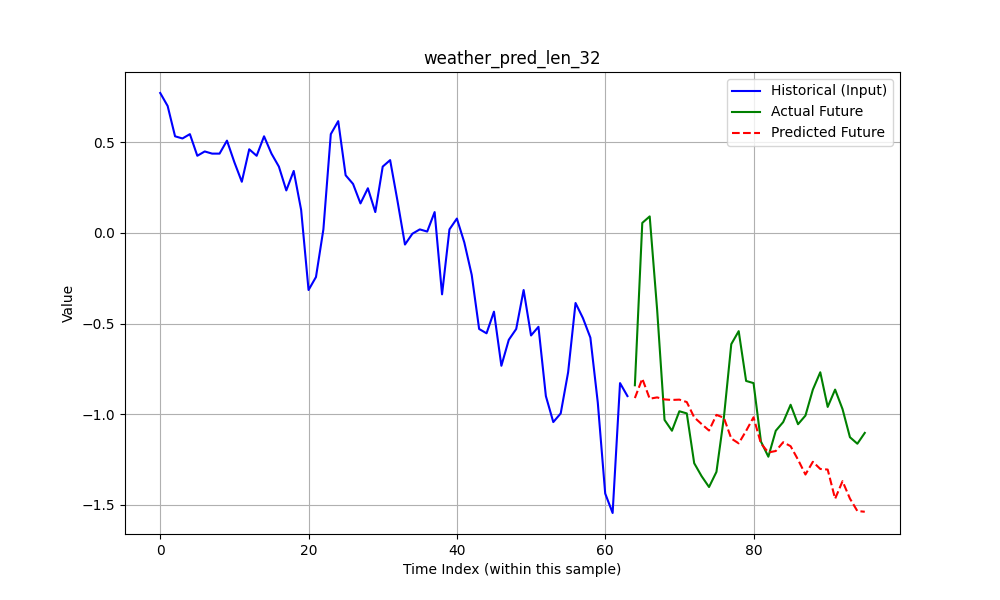
\includegraphics[width=\textwidth]{figures/samformer/weather_pred_len_32_sample_-1.png}
         \caption{Weather - Horizon 32}
    \end{subfigure}
    \begin{subfigure}[b]{0.32\textwidth}
         \centering
         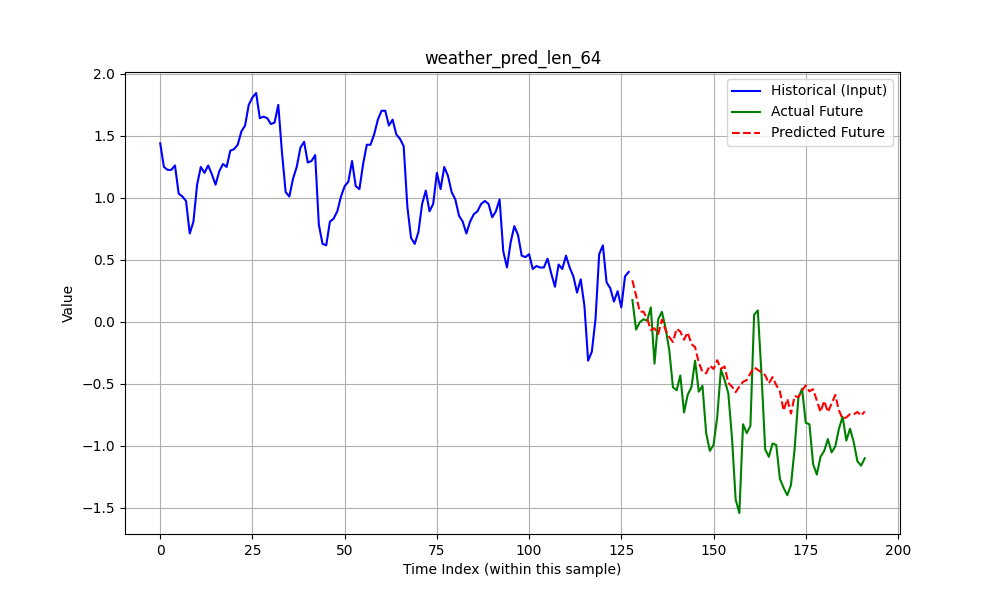
\includegraphics[width=\textwidth]{figures/samformer/weather_pred_len_64_sample_-1.png}
         \caption{Weather - Horizon 64}
    \end{subfigure}
    \begin{subfigure}[b]{0.32\textwidth}
         \centering
         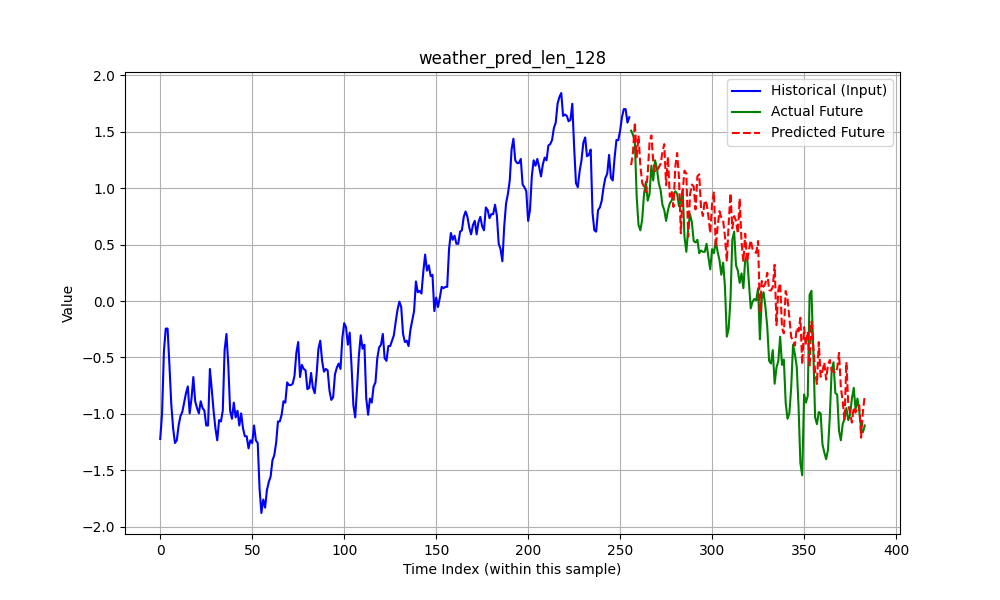
\includegraphics[width=\textwidth]{figures/samformer/weather_pred_len_128_sample_-1.png}
         \caption{Weather - Horizon 128}
    \end{subfigure}
    \caption{SAMFormer predictions on Weather dataset.}
\end{figure}

\begin{figure}[h!]
    \centering
    \begin{subfigure}[b]{0.32\textwidth}
         \centering
         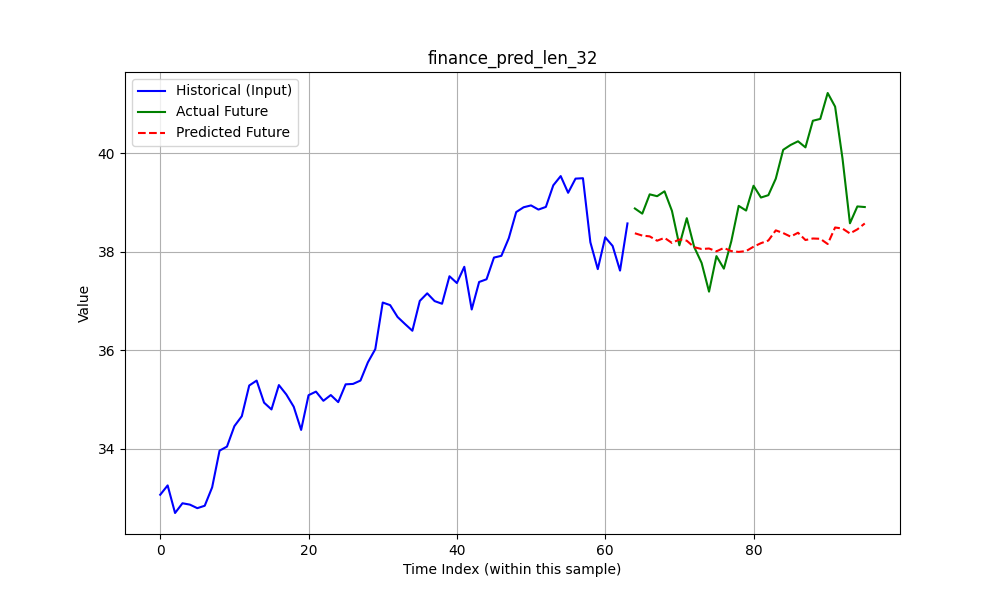
\includegraphics[width=\textwidth]{figures/samformer/finance_pred_len_32_sample_-1.png}
         \caption{Finance - Horizon 32}
    \end{subfigure}
    \begin{subfigure}[b]{0.32\textwidth}
         \centering
         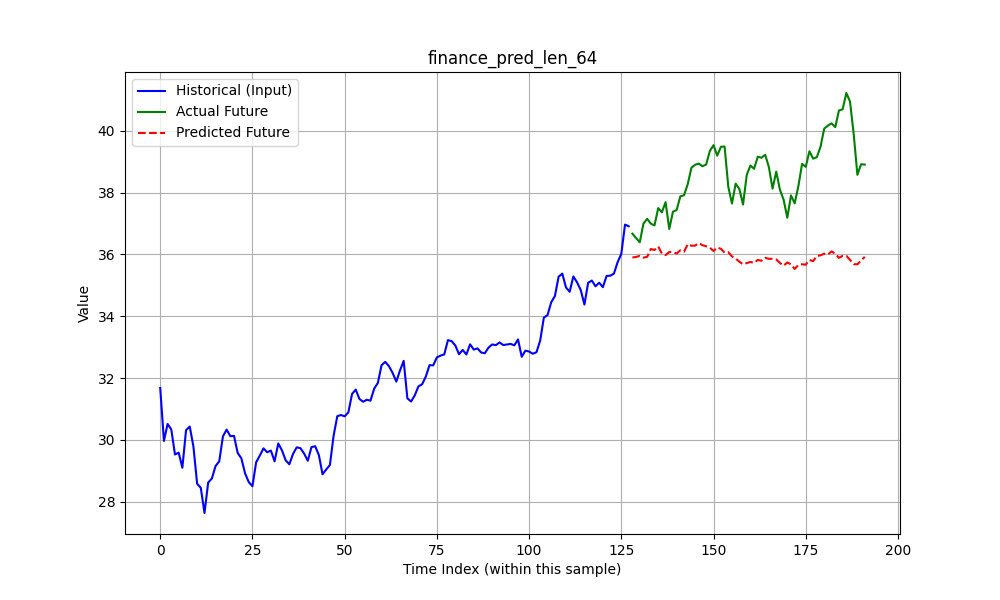
\includegraphics[width=\textwidth]{figures/samformer/finance_pred_len_64_sample_-1.png}
         \caption{Finance - Horizon 64}
    \end{subfigure}
    \begin{subfigure}[b]{0.32\textwidth}
         \centering
         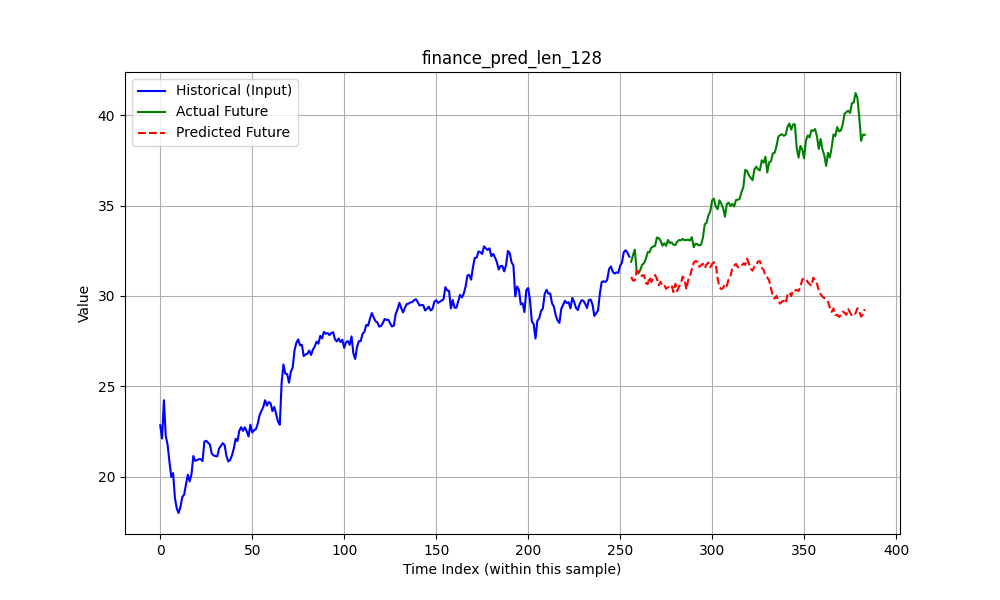
\includegraphics[width=\textwidth]{figures/samformer/finance_pred_len_128_sample_-1.png}
         \caption{Finance - Horizon 128}
    \end{subfigure}
    \caption{SAMFormer predictions on Finance dataset.}
\end{figure}

\begin{figure}[h!]
     \centering
     \begin{subfigure}[b]{0.32\textwidth}
          \centering
          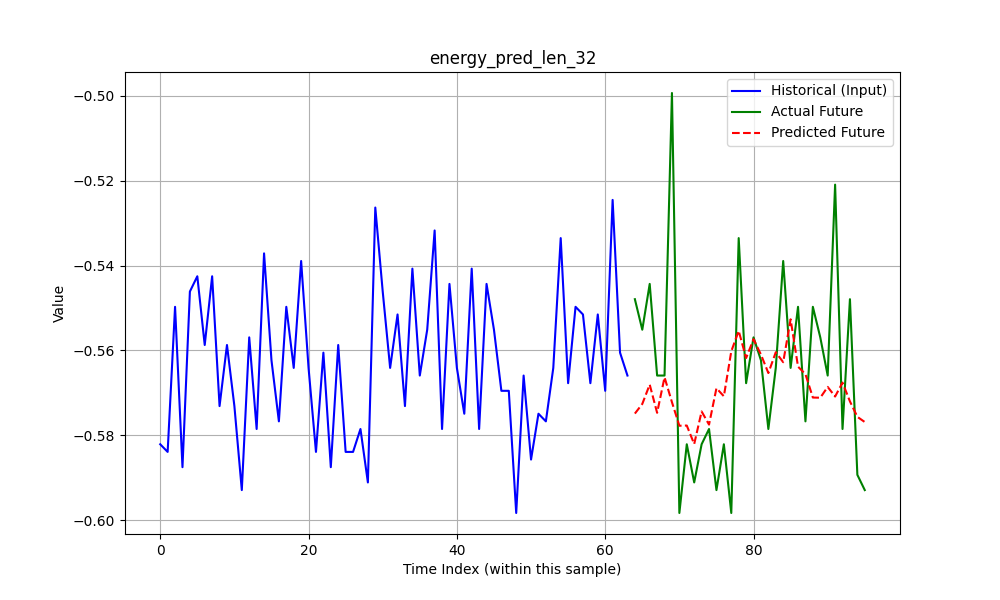
\includegraphics[width=\textwidth]{figures/samformer/energy_pred_len_32_sample_-1.png}
          \caption{Energy - Horizon 32}
     \end{subfigure}
     \begin{subfigure}[b]{0.32\textwidth}
          \centering
          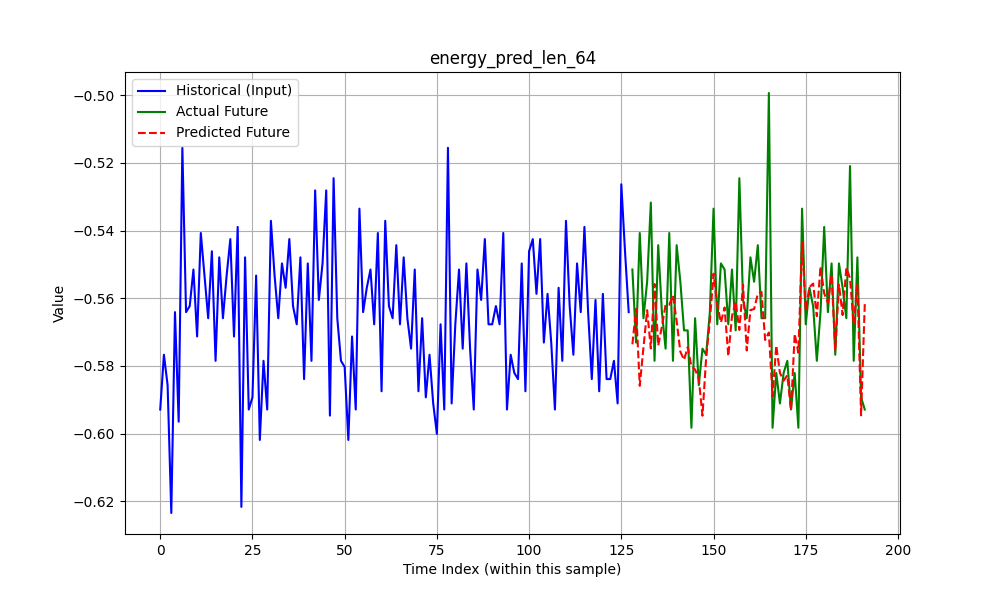
\includegraphics[width=\textwidth]{figures/samformer/energy_pred_len_64_sample_-1.png}
          \caption{Energy - Horizon 64}
     \end{subfigure}
     \begin{subfigure}[b]{0.32\textwidth}
          \centering
          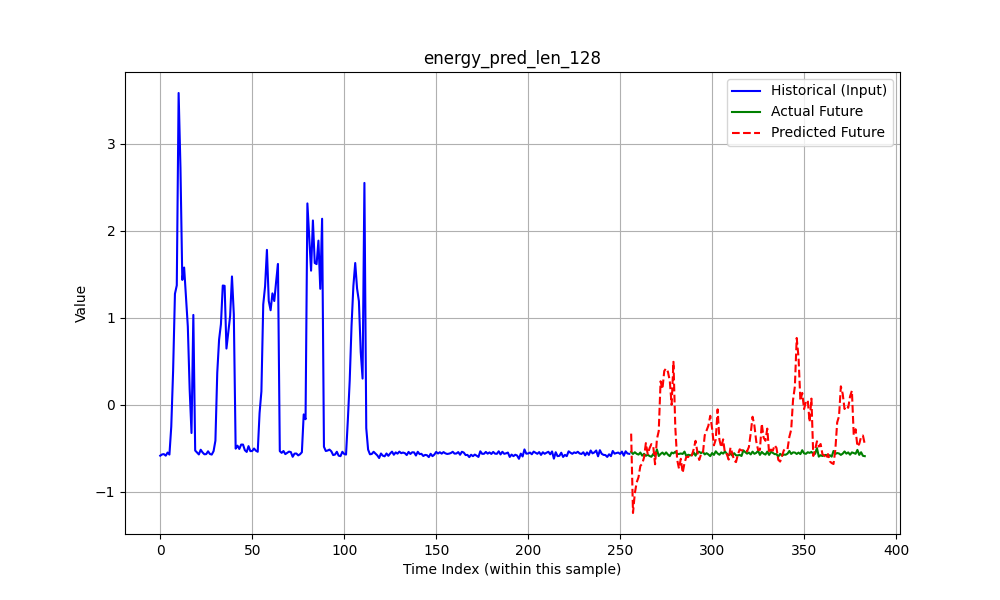
\includegraphics[width=\textwidth]{figures/samformer/energy_pred_len_128_sample_-1.png}
          \caption{Energy - Horizon 128}
     \end{subfigure}
     \caption{SAMFormer predictions on Healthcare dataset.}
 \end{figure}

 \begin{figure}[h!]
     \centering
     \begin{subfigure}[b]{0.32\textwidth}
          \centering
          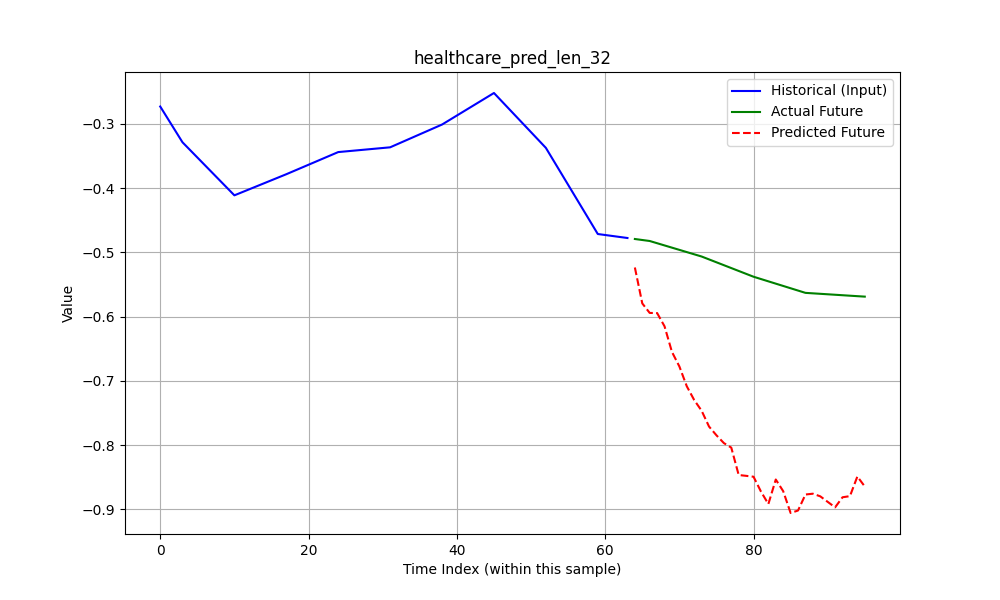
\includegraphics[width=\textwidth]{figures/samformer/healthcare_pred_len_32_sample_-1.png}
          \caption{Healthcare - Horizon 32}
     \end{subfigure}
     \begin{subfigure}[b]{0.32\textwidth}
          \centering
          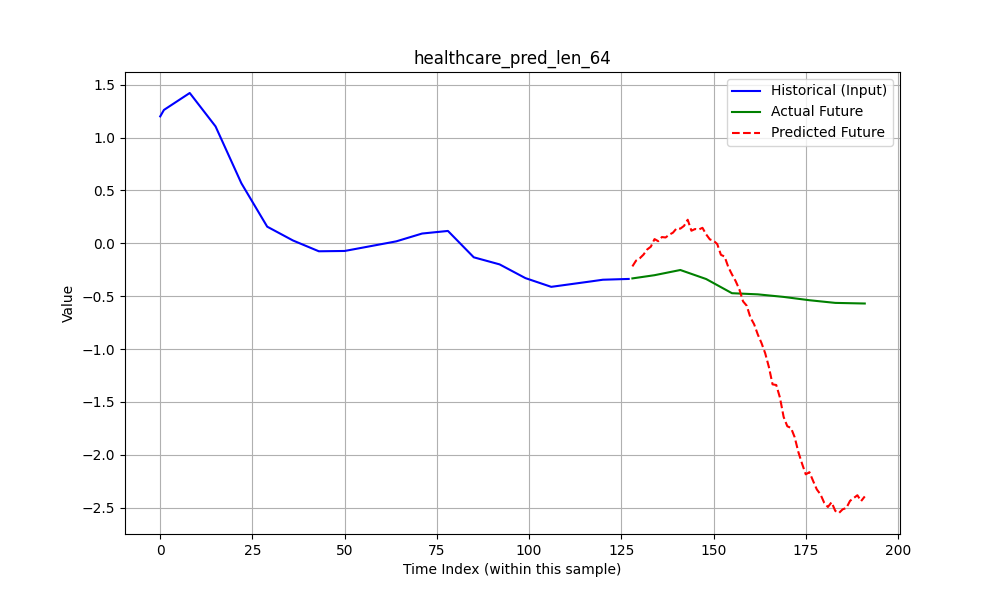
\includegraphics[width=\textwidth]{figures/samformer/healthcare_pred_len_64_sample_-1.png}
          \caption{Healthcare - Horizon 64}
     \end{subfigure}
     \begin{subfigure}[b]{0.32\textwidth}
          \centering
          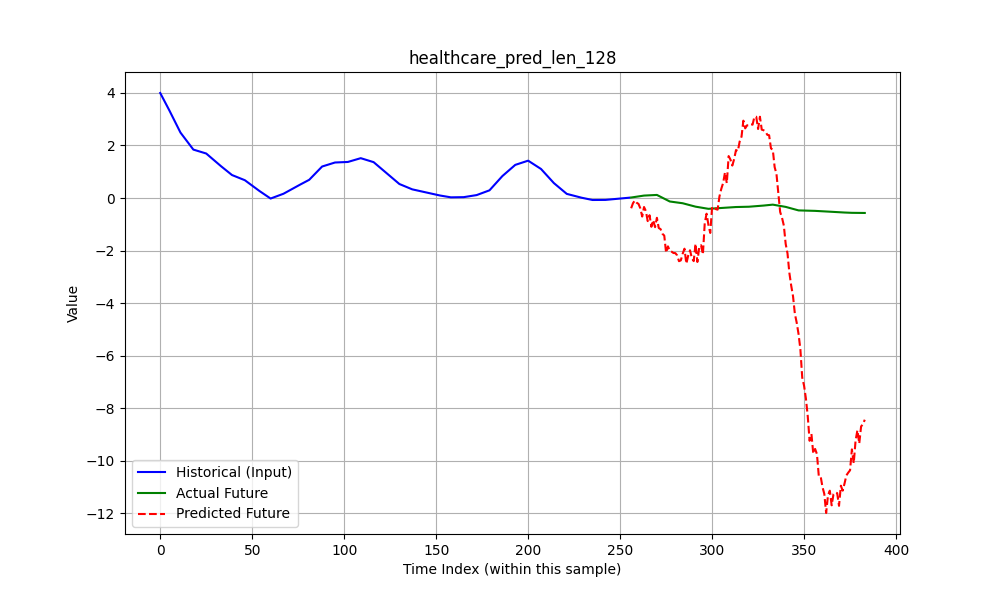
\includegraphics[width=\textwidth]{figures/samformer/healthcare_pred_len_128_sample_-1.png}
          \caption{Healthcare - Horizon 128}
     \end{subfigure}
     \caption{SAMFormer predictions on Healthcare dataset.}
 \end{figure}

\subsection{TimesFM}
\begin{figure}[h!]
    \centering
    \begin{subfigure}[b]{0.32\textwidth}
         \centering
         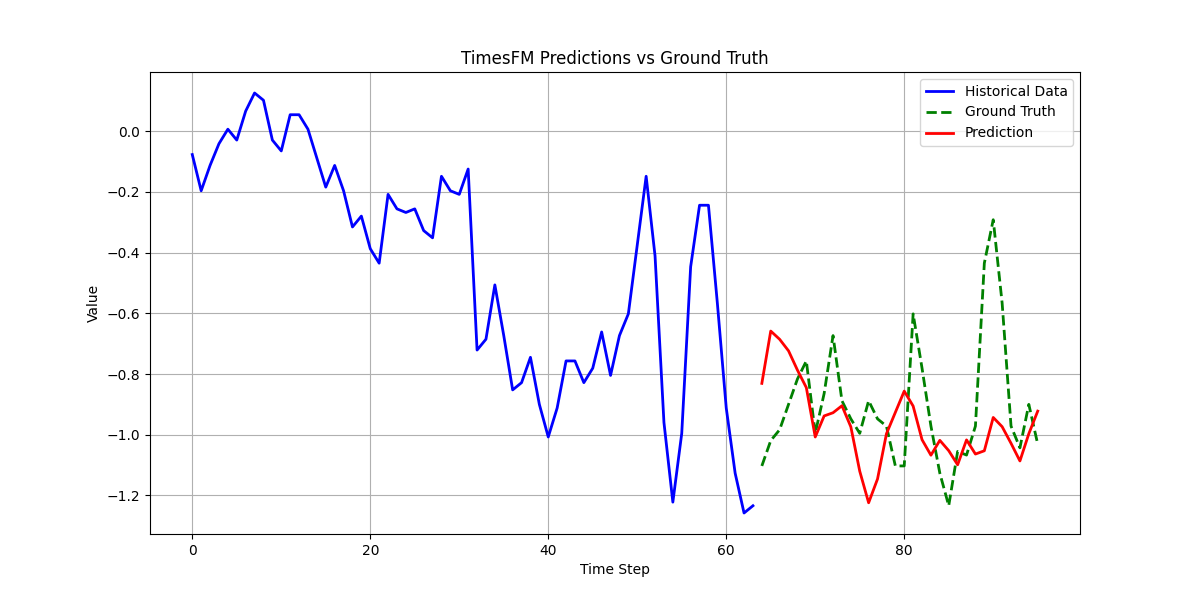
\includegraphics[width=\textwidth]{figures/timesfm/weather_predictions_exp1.png}
         \caption{Weather - Exp 1}
    \end{subfigure}
    \begin{subfigure}[b]{0.32\textwidth}
         \centering
         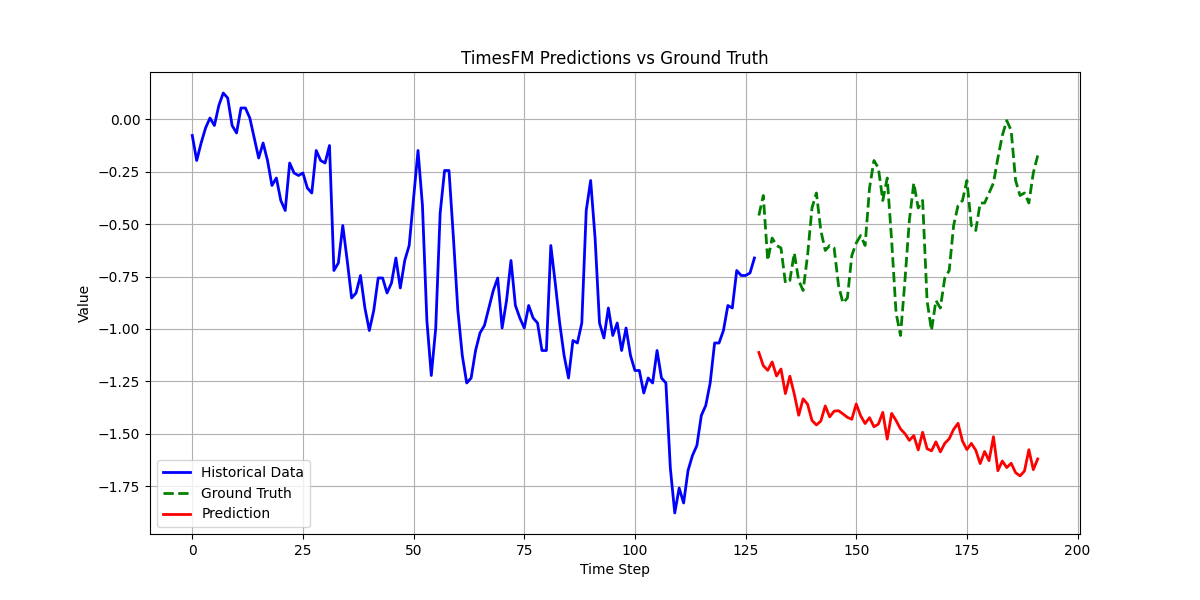
\includegraphics[width=\textwidth]{figures/timesfm/weather_predictions_exp2.png}
         \caption{Weather - Exp 2}
    \end{subfigure}
    \begin{subfigure}[b]{0.32\textwidth}
         \centering
         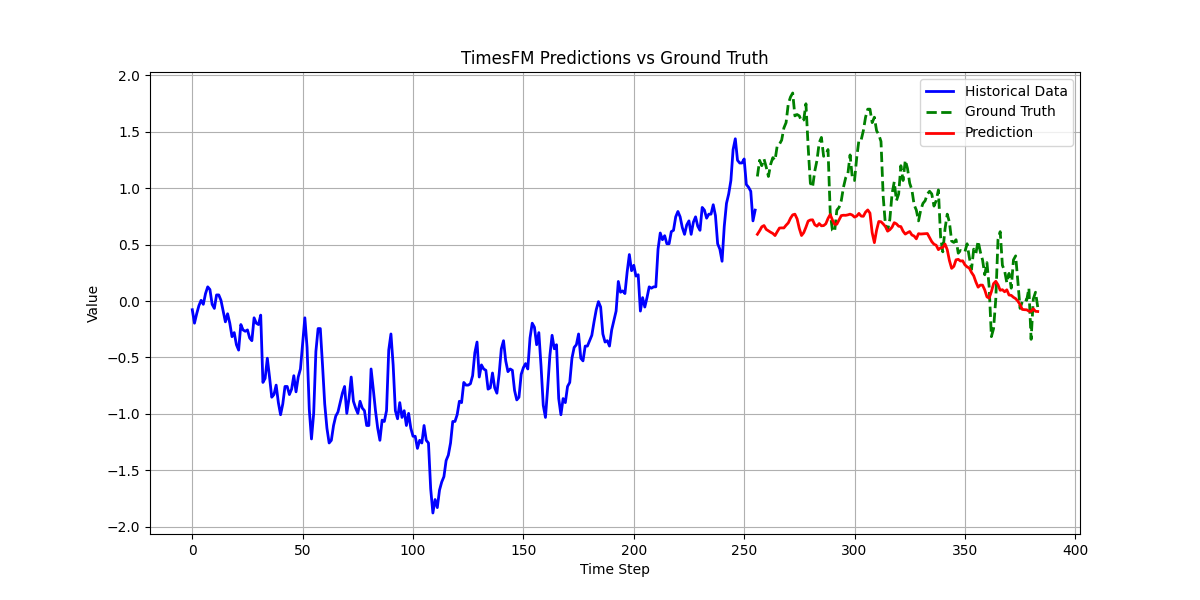
\includegraphics[width=\textwidth]{figures/timesfm/weather_predictions_exp3.png}
         \caption{Weather - Exp 3}
    \end{subfigure}
    \caption{TimesFM predictions on Weather dataset.}
\end{figure}

\begin{figure}[h!]
     \centering
     \begin{subfigure}[b]{0.32\textwidth}
          \centering
          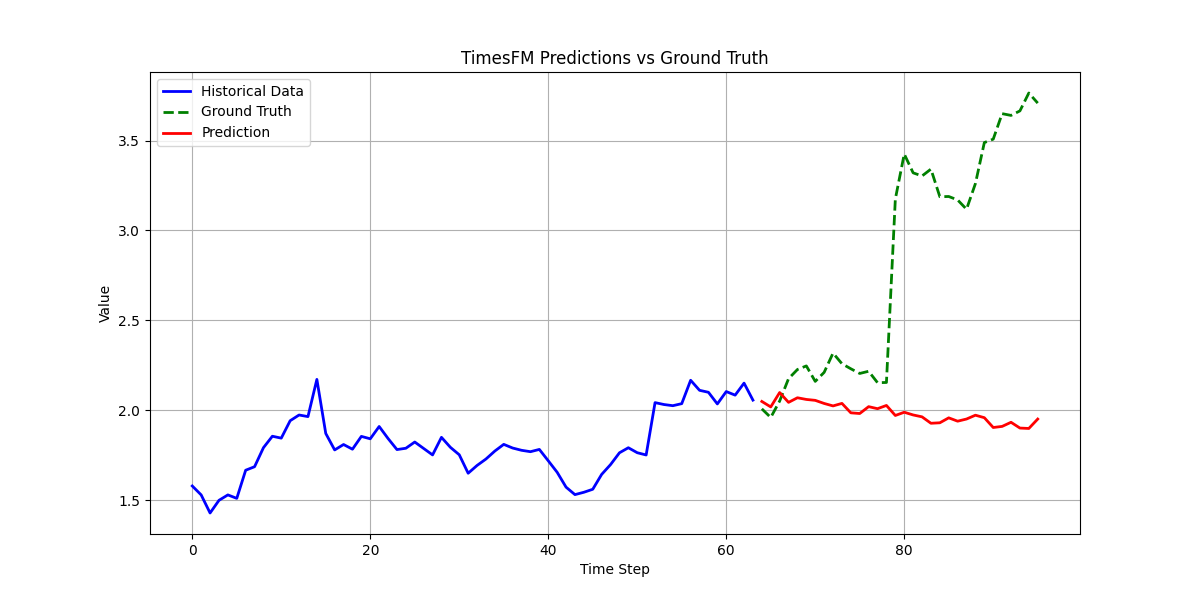
\includegraphics[width=\textwidth]{figures/timesfm/finance_predictions_exp1.png}
          \caption{Finance - Exp 1}
     \end{subfigure}
     \begin{subfigure}[b]{0.32\textwidth}
          \centering
          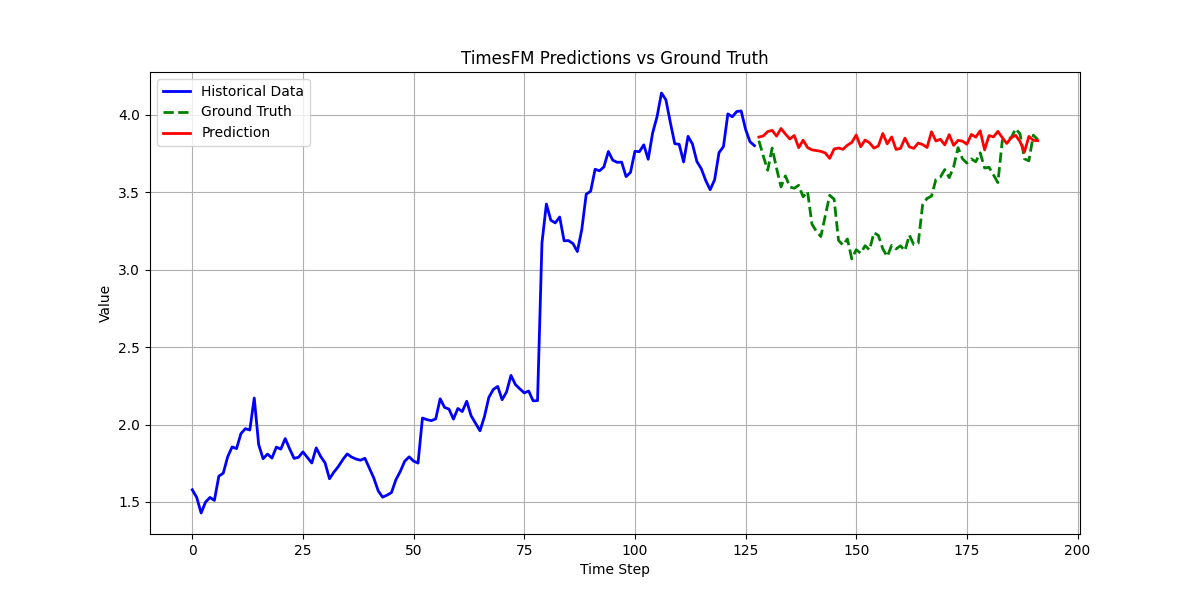
\includegraphics[width=\textwidth]{figures/timesfm/finance_predictions_exp2.png}
          \caption{Finance - Exp 2}
     \end{subfigure}
     \begin{subfigure}[b]{0.32\textwidth}
          \centering
          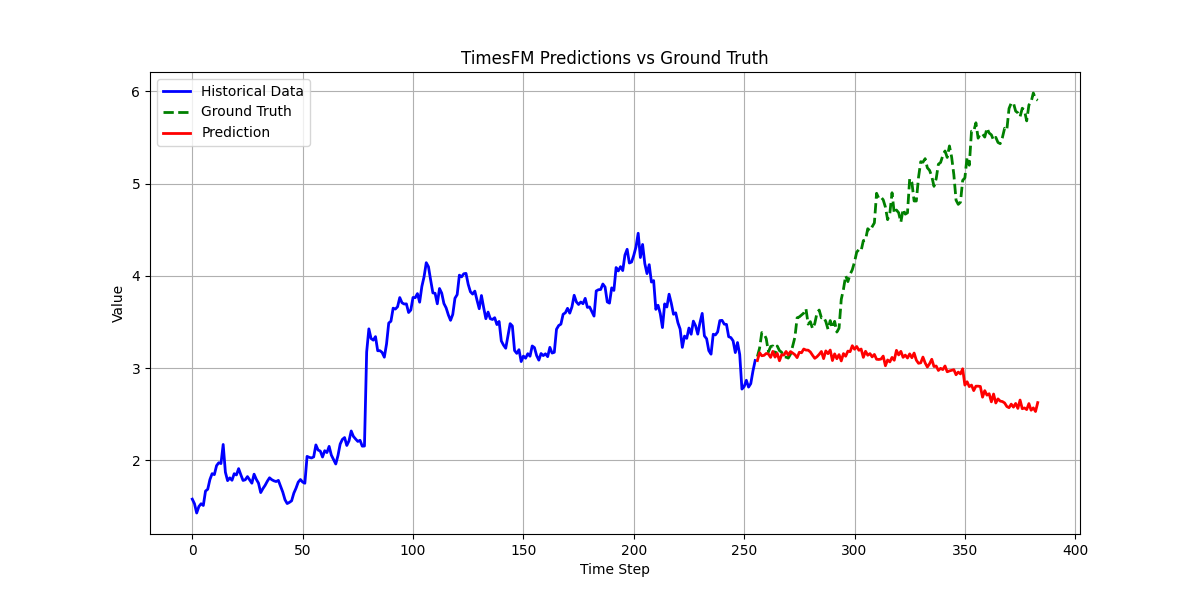
\includegraphics[width=\textwidth]{figures/timesfm/finance_predictions_exp3.png}
          \caption{Finance - Exp 3}
     \end{subfigure}
     \caption{TimesFM predictions on Finance dataset.}
 \end{figure}

 \begin{figure}[h!]
     \centering
     \begin{subfigure}[b]{0.32\textwidth}
          \centering
          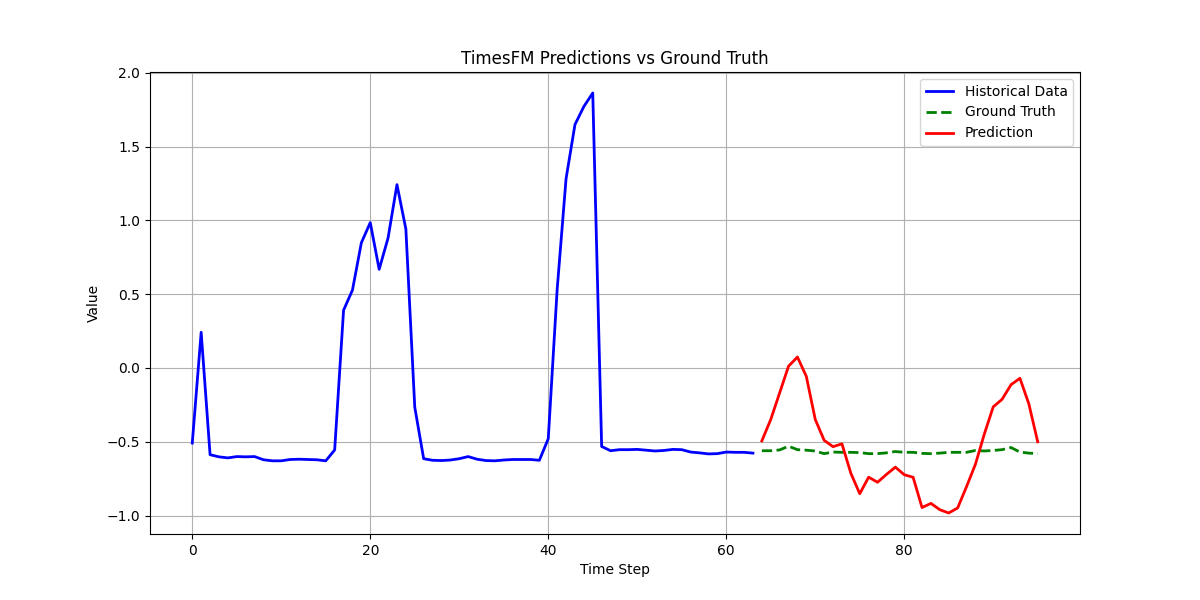
\includegraphics[width=\textwidth]{figures/timesfm/energy_predictions_exp1.png}
          \caption{Energy - Exp 1}
     \end{subfigure}
     \begin{subfigure}[b]{0.32\textwidth}
          \centering
          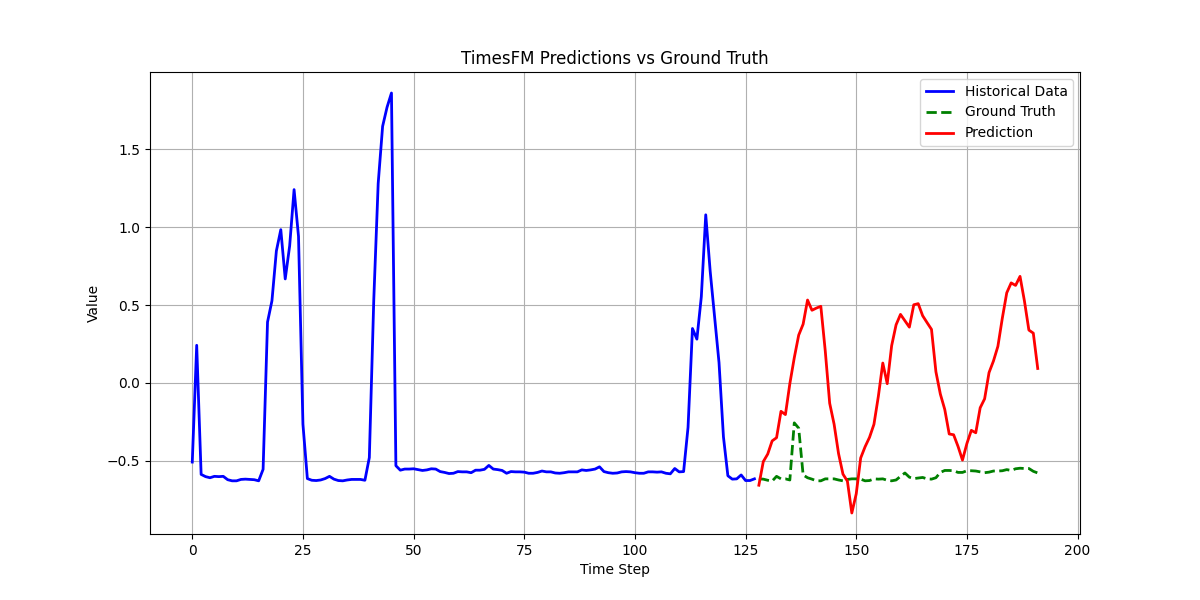
\includegraphics[width=\textwidth]{figures/timesfm/energy_predictions_exp2.png}
          \caption{Energy - Exp 2}
     \end{subfigure}
     \begin{subfigure}[b]{0.32\textwidth}
          \centering
          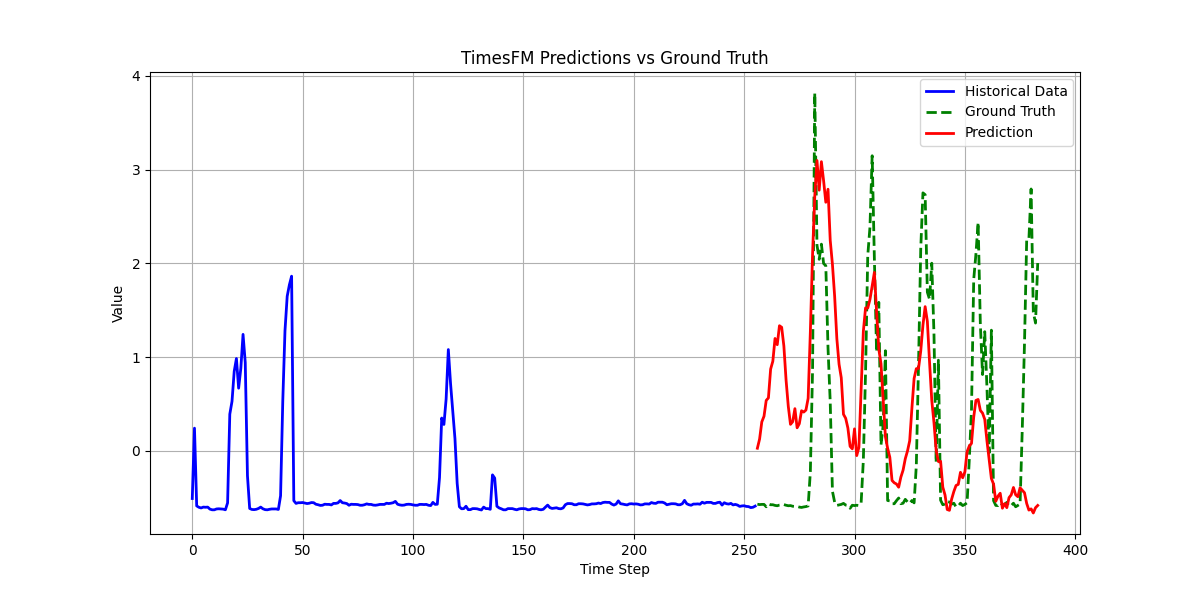
\includegraphics[width=\textwidth]{figures/timesfm/energy_predictions_exp3.png}
          \caption{Energy - Exp 3}
     \end{subfigure}
     \caption{TimesFM predictions on Energy dataset.}
 \end{figure}

 \begin{figure}[h!]
     \centering
     \begin{subfigure}[b]{0.32\textwidth}
          \centering
          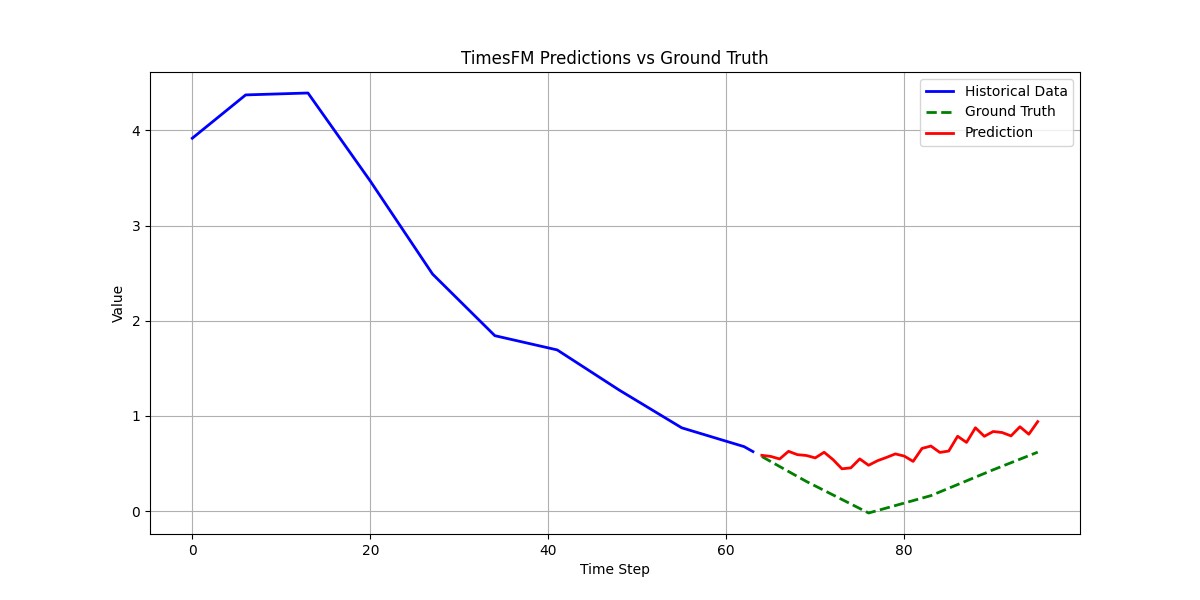
\includegraphics[width=\textwidth]{figures/timesfm/healthcare_predictions_exp1.png}
          \caption{Healthcare - Exp 1}
     \end{subfigure}
     \begin{subfigure}[b]{0.32\textwidth}
          \centering
          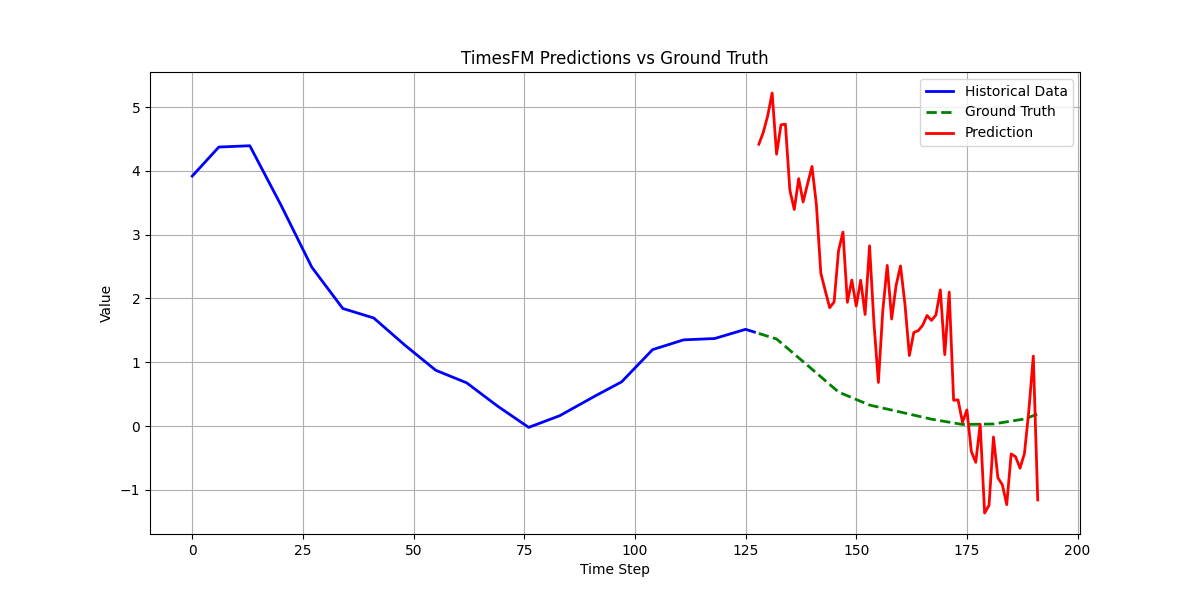
\includegraphics[width=\textwidth]{figures/timesfm/healthcare_predictions_exp2.png}
          \caption{Healthcare - Exp 2}
     \end{subfigure}
     \begin{subfigure}[b]{0.32\textwidth}
          \centering
          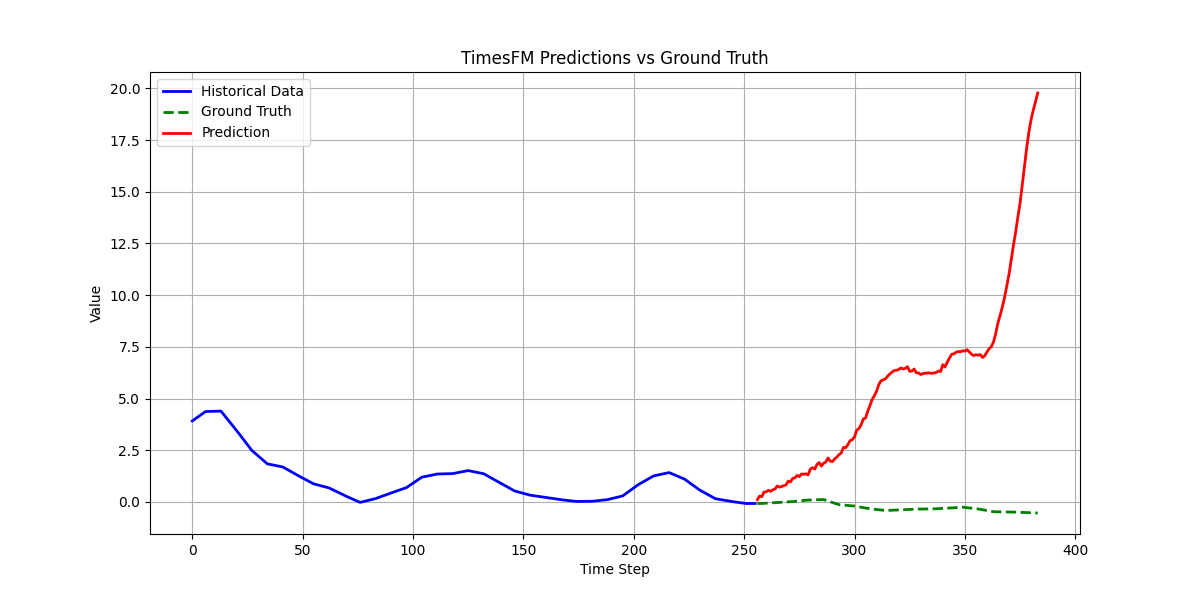
\includegraphics[width=\textwidth]{figures/timesfm/healthcare_predictions_exp3.png}
          \caption{Healhcare - Exp 3}
     \end{subfigure}
     \caption{TimesFM predictions on Healhcare dataset.}
 \end{figure}

\subsection{TimeGPT}
\begin{figure}[h!]
    \centering
    \begin{subfigure}[b]{0.32\textwidth}
         \centering
         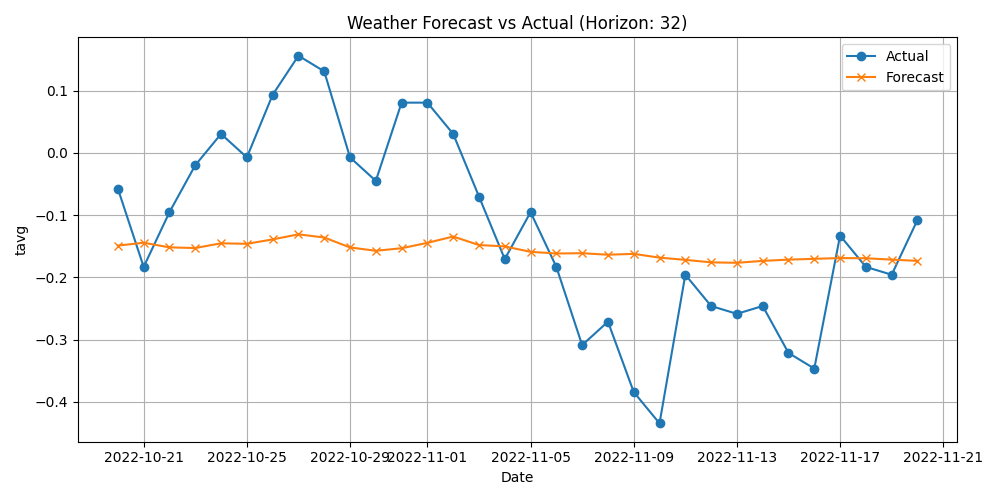
\includegraphics[width=\textwidth]{figures/timegpt/weather_32_forecast_plot.png}
         \caption{Weather - Horizon 32}
    \end{subfigure}
    \begin{subfigure}[b]{0.32\textwidth}
         \centering
         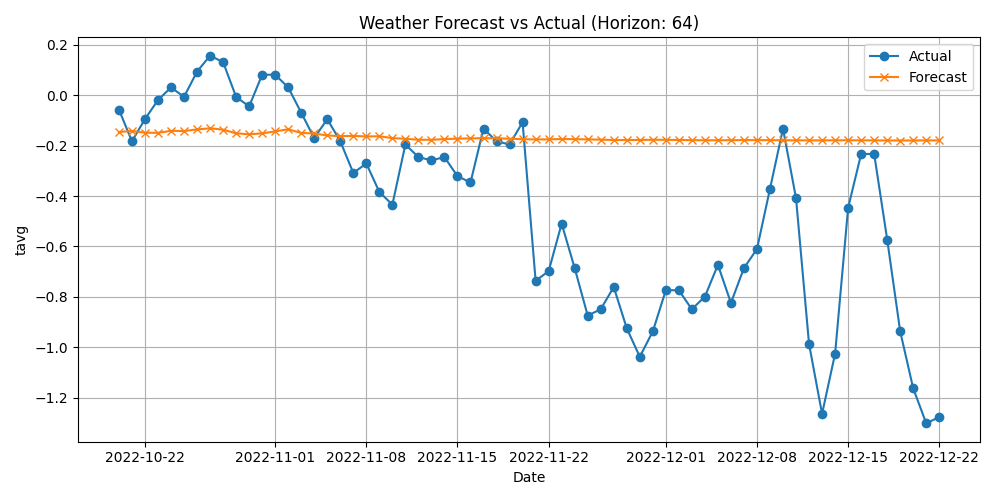
\includegraphics[width=\textwidth]{figures/timegpt/weather_64_forecast_plot.png}
         \caption{Weather - Horizon 64}
    \end{subfigure}
    \begin{subfigure}[b]{0.32\textwidth}
         \centering
         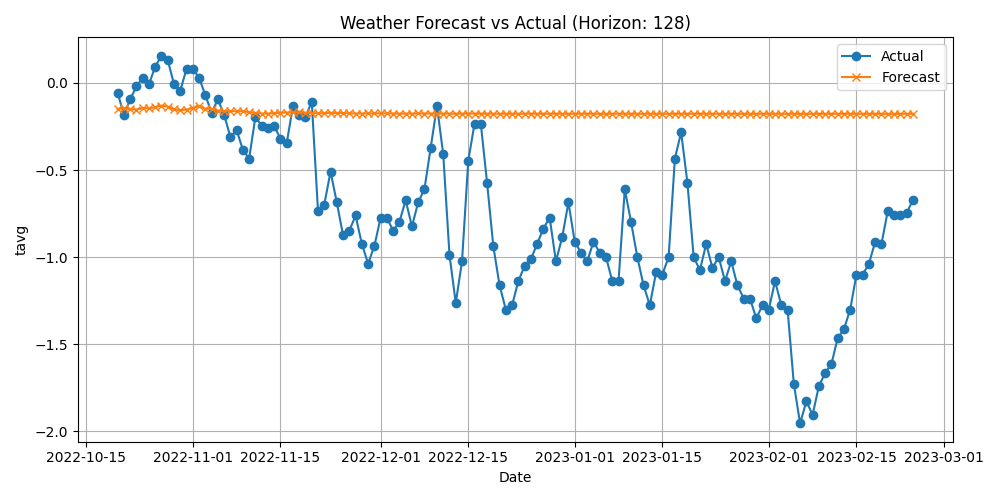
\includegraphics[width=\textwidth]{figures/timegpt/weather_128_forecast_plot.png}
         \caption{Weather - Horizon 128}
    \end{subfigure}
    \caption{TimeGPT predictions on Weather dataset.}
\end{figure}

\begin{figure}[h!]
     \centering
     \begin{subfigure}[b]{0.32\textwidth}
          \centering
          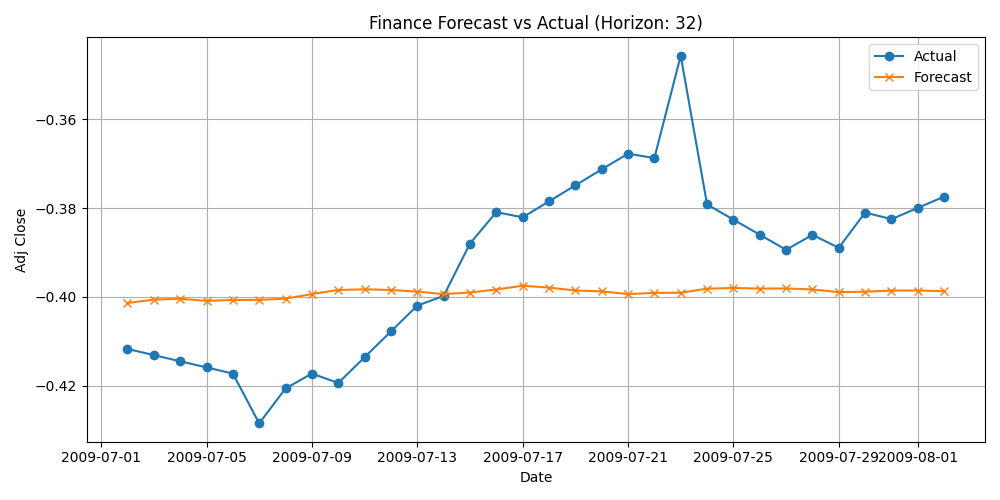
\includegraphics[width=\textwidth]{figures/timegpt/finance_32_forecast_plot.png}
          \caption{Finance - Horizon 32}
     \end{subfigure}
     \begin{subfigure}[b]{0.32\textwidth}
          \centering
          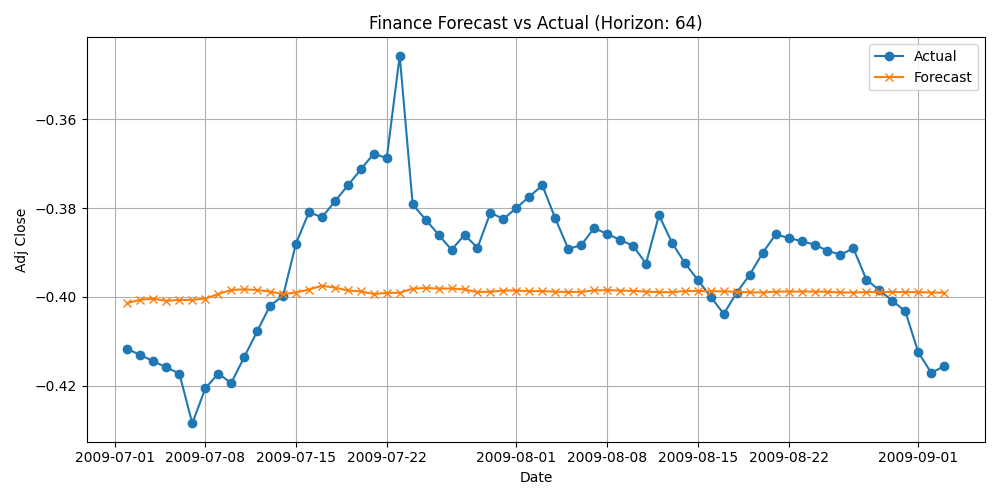
\includegraphics[width=\textwidth]{figures/timegpt/finance_64_forecast_plot.png}
          \caption{Finance - Horizon 64}
     \end{subfigure}
     \begin{subfigure}[b]{0.32\textwidth}
          \centering
          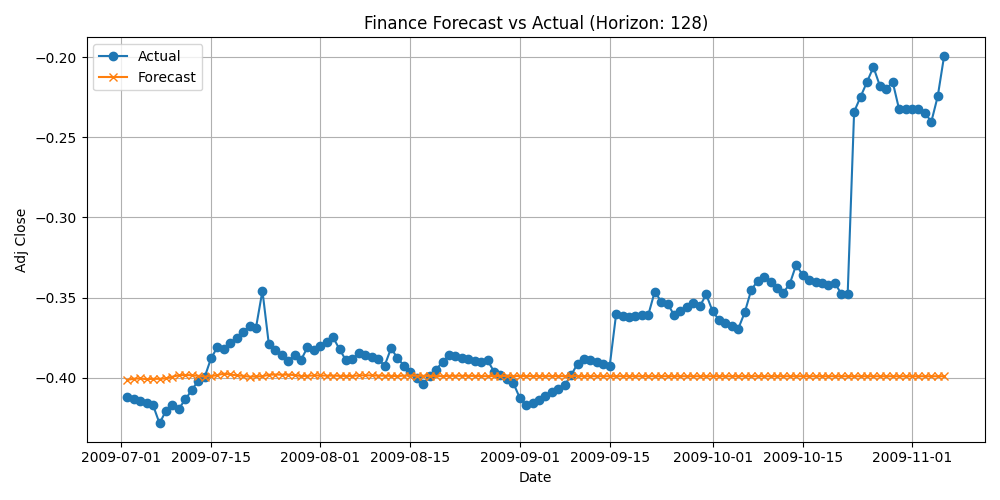
\includegraphics[width=\textwidth]{figures/timegpt/finance_128_forecast_plot.png}
          \caption{Finance - Horizon 128}
     \end{subfigure}
     \caption{TimeGPT predictions on Finance dataset.}
 \end{figure}

 \begin{figure}[h!]
     \centering
     \begin{subfigure}[b]{0.32\textwidth}
          \centering
          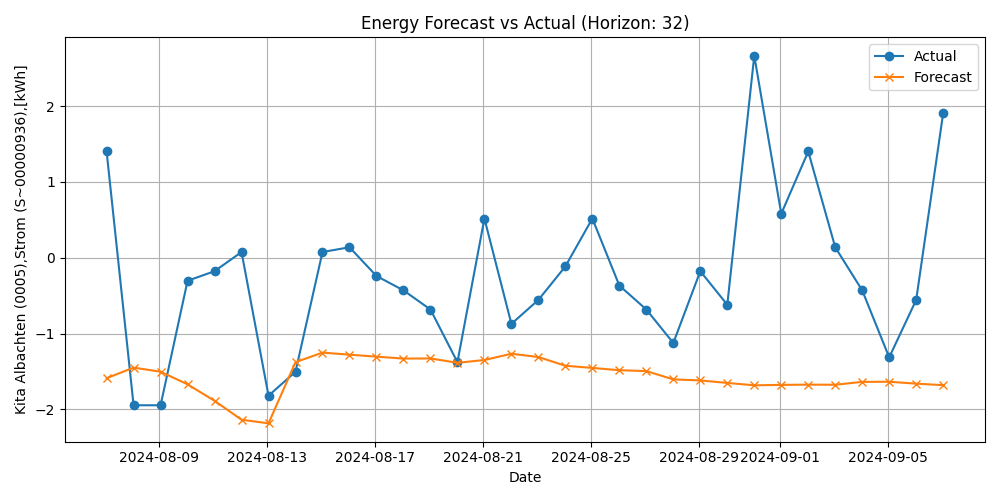
\includegraphics[width=\textwidth]{figures/timegpt/energy_32_forecast_plot.png}
          \caption{Energy - Horizon 32}
     \end{subfigure}
     \begin{subfigure}[b]{0.32\textwidth}
          \centering
          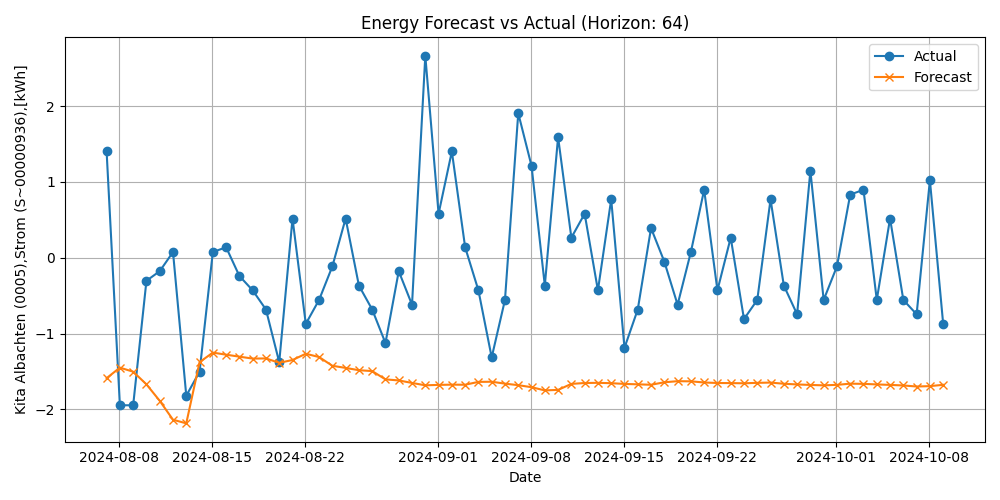
\includegraphics[width=\textwidth]{figures/timegpt/energy_64_forecast_plot.png}
          \caption{Energy - Horizon 64}
     \end{subfigure}
     \begin{subfigure}[b]{0.32\textwidth}
          \centering
          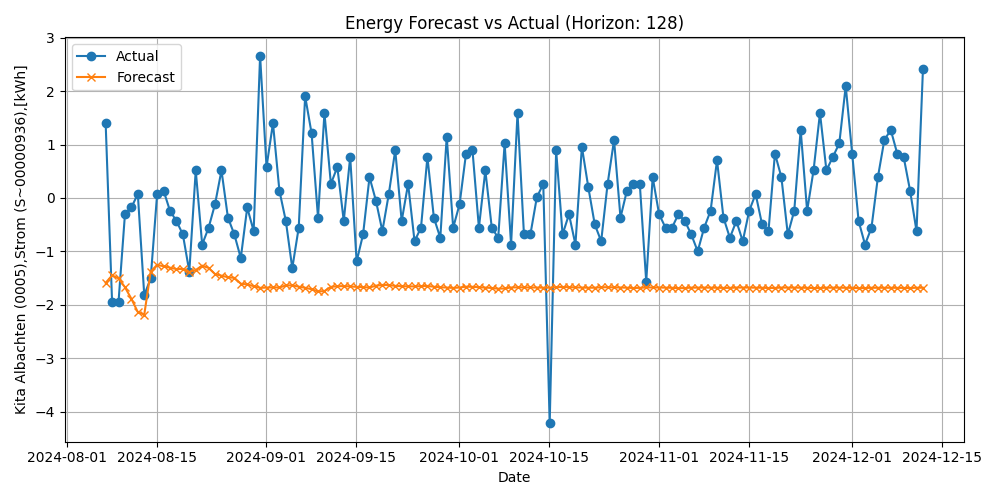
\includegraphics[width=\textwidth]{figures/timegpt/energy_128_forecast_plot.png}
          \caption{Energy - Horizon 128}
     \end{subfigure}
     \caption{TimeGPT predictions on Energy dataset.}
 \end{figure}

 \begin{figure}[h!]
     \centering
     \begin{subfigure}[b]{0.32\textwidth}
          \centering
          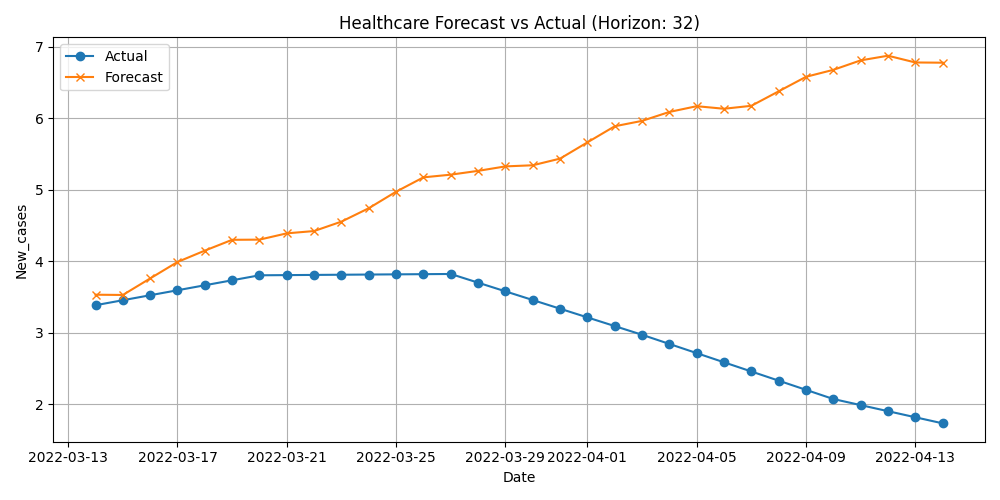
\includegraphics[width=\textwidth]{figures/timegpt/healthcare_32_forecast_plot.png}
          \caption{Healthcare - Horizon 32}
     \end{subfigure}
     \begin{subfigure}[b]{0.32\textwidth}
          \centering
          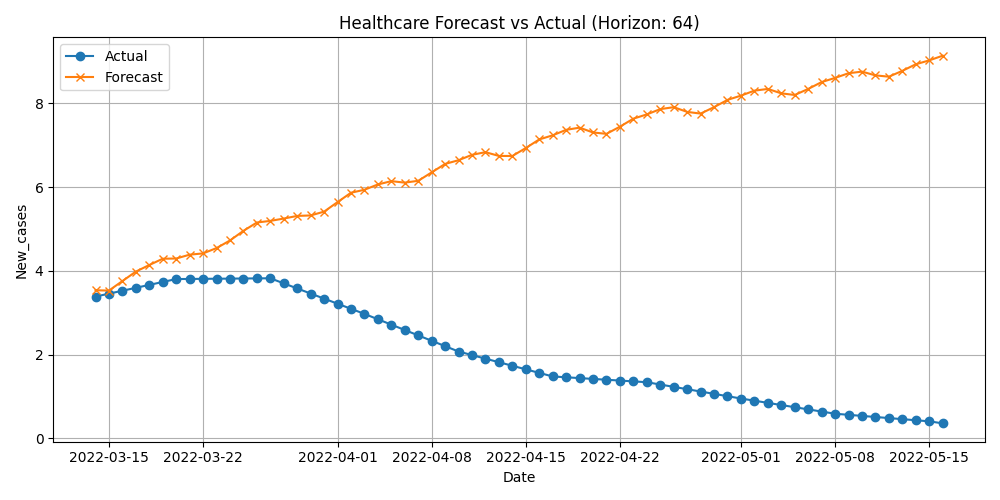
\includegraphics[width=\textwidth]{figures/timegpt/healthcare_64_forecast_plot.png}
          \caption{Healthcare - Horizon 64}
     \end{subfigure}
     \begin{subfigure}[b]{0.32\textwidth}
          \centering
          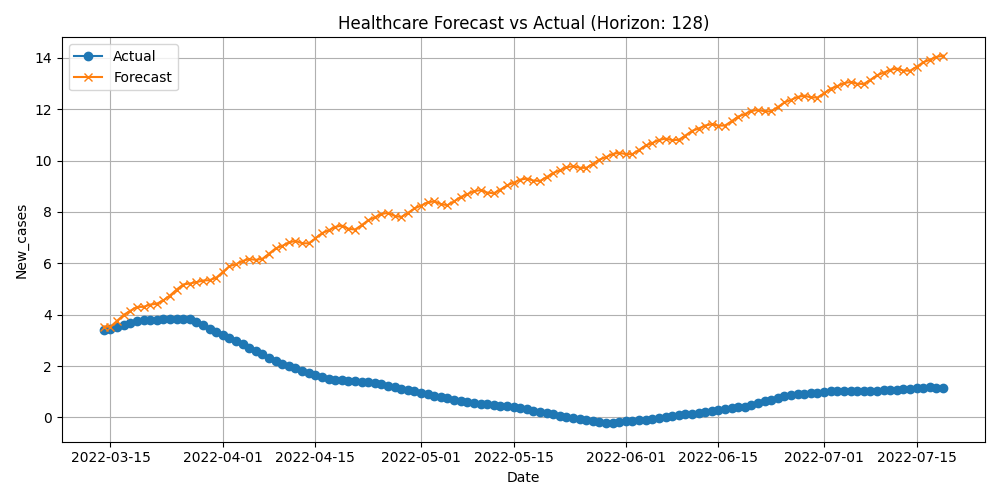
\includegraphics[width=\textwidth]{figures/timegpt/healthcare_128_forecast_plot.png}
          \caption{Healthcare - Horizon 128}
     \end{subfigure}
     \caption{TimeGPT predictions on Healthcare dataset.}
 \end{figure}

\subsection{Time-MoE}
\begin{figure}[h!]
    \centering
    \begin{subfigure}[b]{0.32\textwidth}
         \centering
         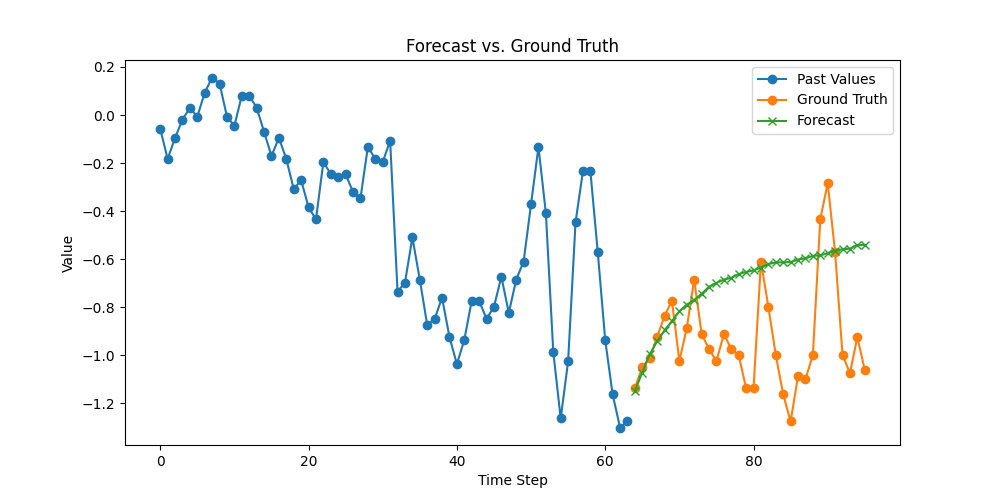
\includegraphics[width=\textwidth]{figures/time-moe/lezhe_64_32.png}
         \caption{Weather - Horizon 64$\to$32}
    \end{subfigure}
    \begin{subfigure}[b]{0.32\textwidth}
         \centering
         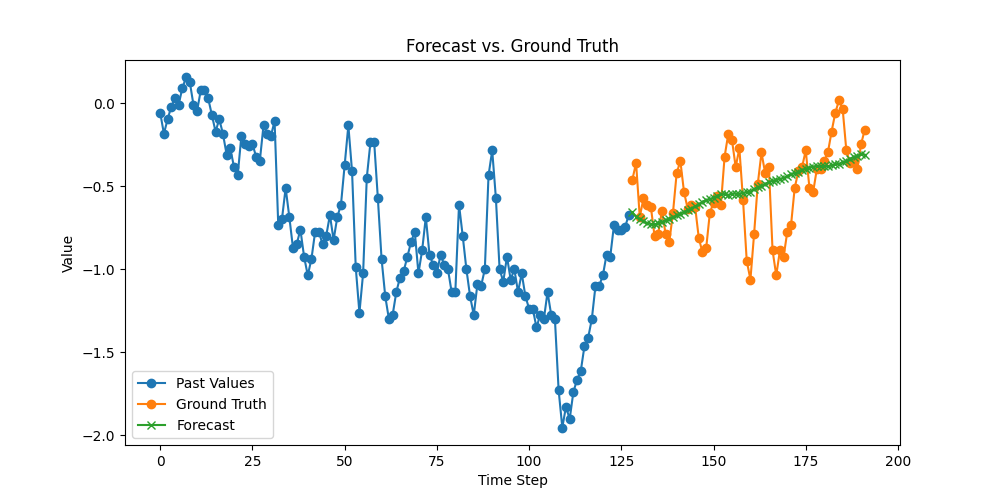
\includegraphics[width=\textwidth]{figures/time-moe/lezhe_128_64.png}
         \caption{Weather - Horizon 128$\to$64}
    \end{subfigure}
    \begin{subfigure}[b]{0.32\textwidth}
         \centering
         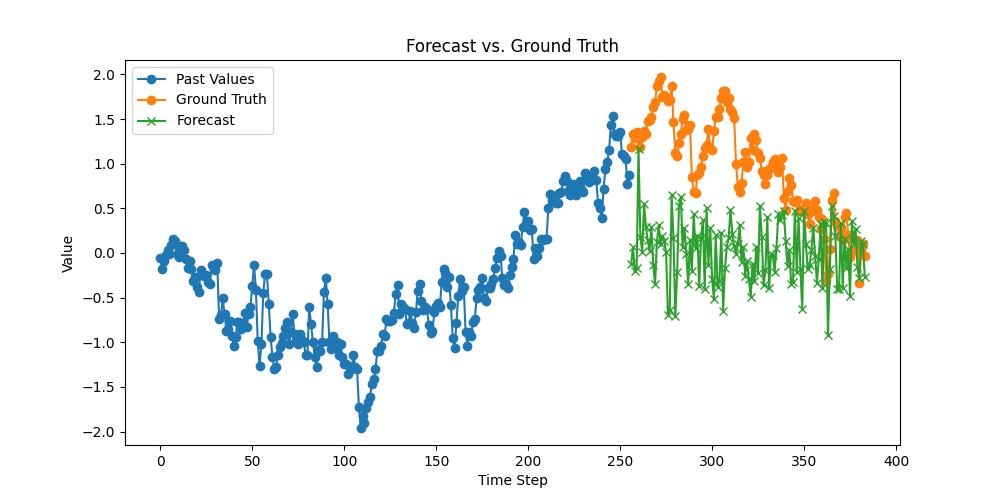
\includegraphics[width=\textwidth]{figures/time-moe/lezhe_256_128.png}
         \caption{Weather - Horizon 256$\to$128}
    \end{subfigure}
    \caption{Time-MoE predictions on Weather dataset.}
\end{figure}

\begin{figure}[h!]
     \centering
     \begin{subfigure}[b]{0.32\textwidth}
          \centering
          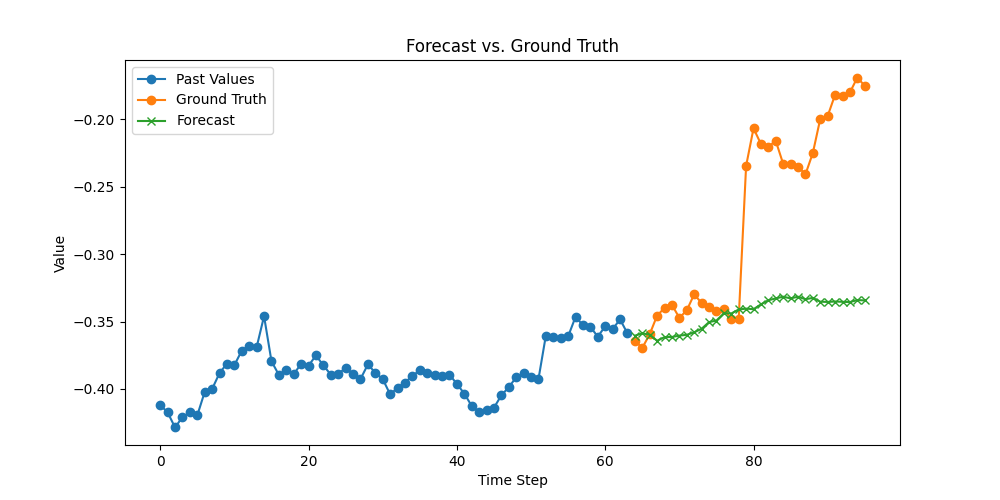
\includegraphics[width=\textwidth]{figures/time-moe/finance_64_32.png}
          \caption{Finance - Horizon 64$\to$32}
     \end{subfigure}
     \begin{subfigure}[b]{0.32\textwidth}
          \centering
          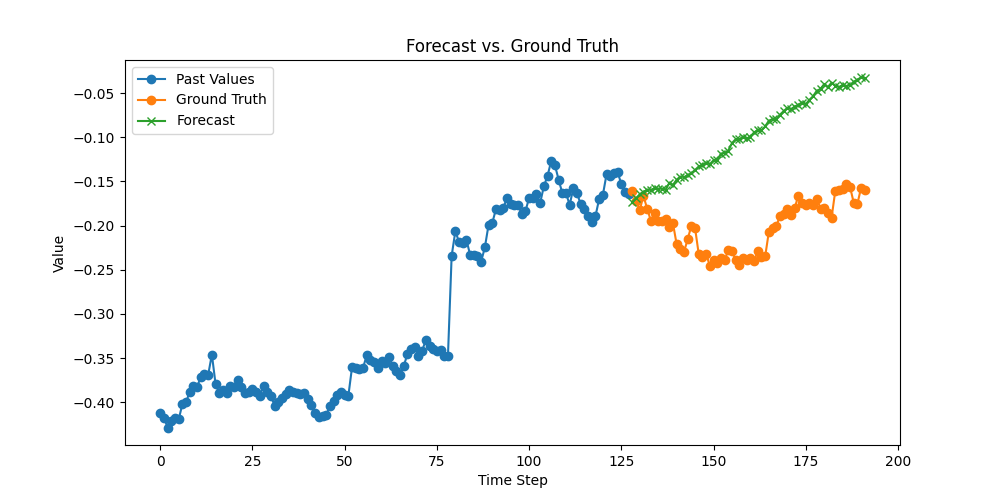
\includegraphics[width=\textwidth]{figures/time-moe/finance_128_64.png}
          \caption{Finance - Horizon 128$\to$64}
     \end{subfigure}
     \begin{subfigure}[b]{0.32\textwidth}
          \centering
          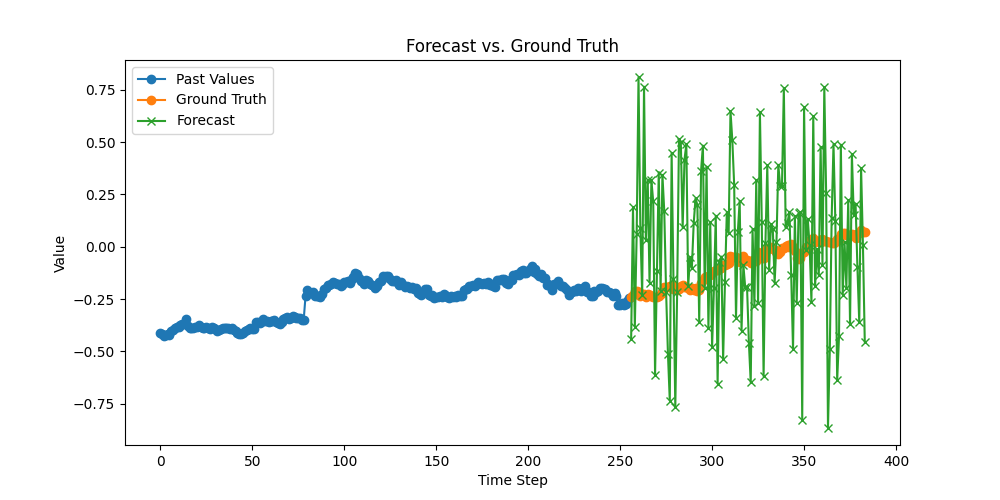
\includegraphics[width=\textwidth]{figures/time-moe/finance_256_128.png}
          \caption{Finance - Horizon 256$\to$128}
     \end{subfigure}
     \caption{Time-MoE predictions on Finance dataset.}
 \end{figure}

 \begin{figure}[h!]
     \centering
     \begin{subfigure}[b]{0.32\textwidth}
          \centering
          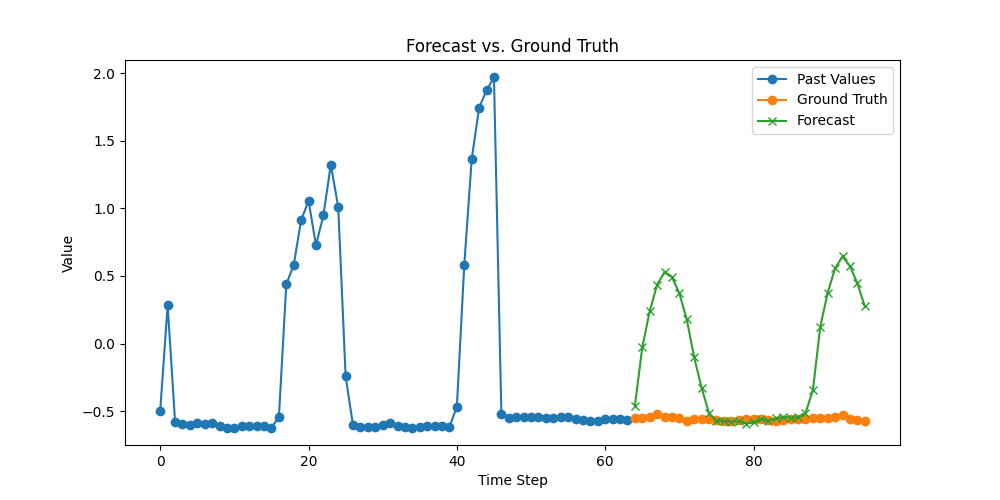
\includegraphics[width=\textwidth]{figures/time-moe/energy_64_32.png}
          \caption{Energy - Horizon 64$\to$32}
     \end{subfigure}
     \begin{subfigure}[b]{0.32\textwidth}
          \centering
          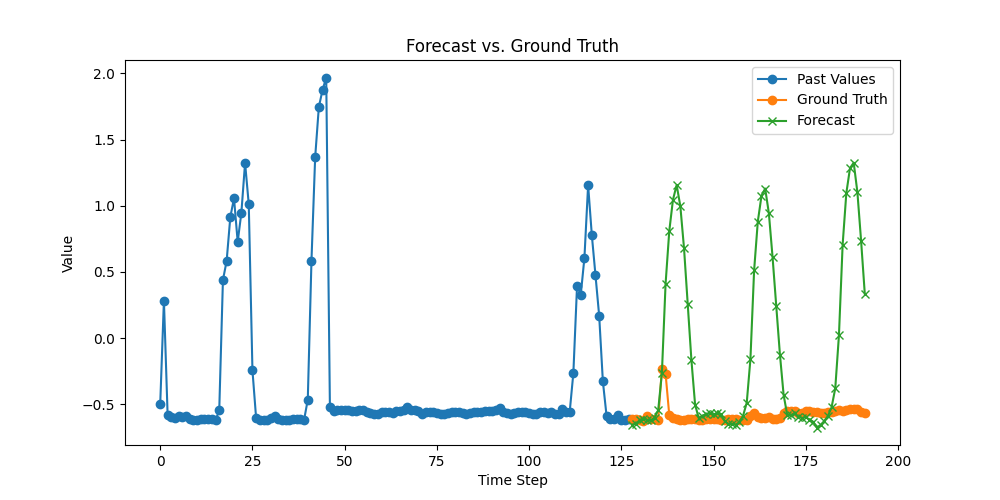
\includegraphics[width=\textwidth]{figures/time-moe/energy_128_64.png}
          \caption{Energy - Horizon 128$\to$64}
     \end{subfigure}
     \begin{subfigure}[b]{0.32\textwidth}
          \centering
          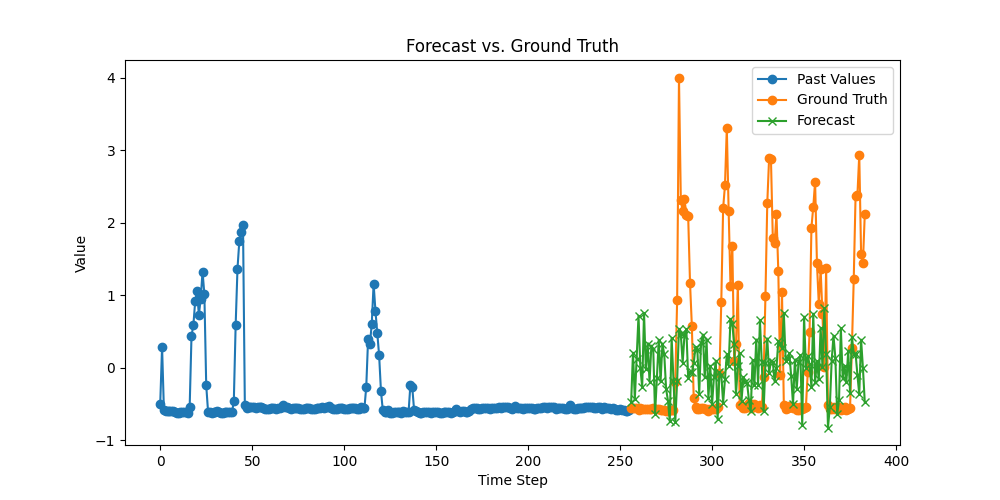
\includegraphics[width=\textwidth]{figures/time-moe/energy_256_128.png}
          \caption{Energy - Horizon 256$\to$128}
     \end{subfigure}
     \caption{Time-MoE predictions on Energy dataset.}
 \end{figure}

 \begin{figure}[h!]
     \centering
     \begin{subfigure}[b]{0.32\textwidth}
          \centering
          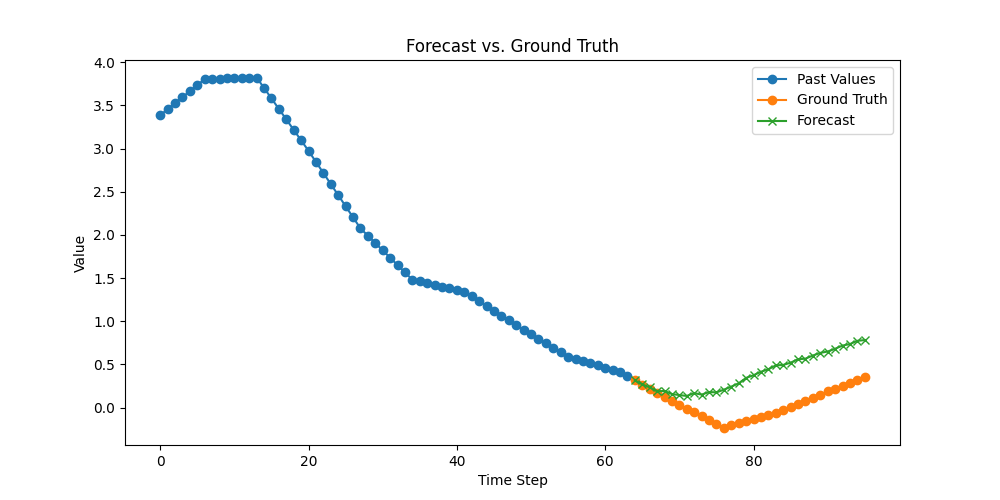
\includegraphics[width=\textwidth]{figures/time-moe/Germany_64_32.png}
          \caption{Healthcare - Horizon 64$\to$32}
     \end{subfigure}
     \begin{subfigure}[b]{0.32\textwidth}
          \centering
          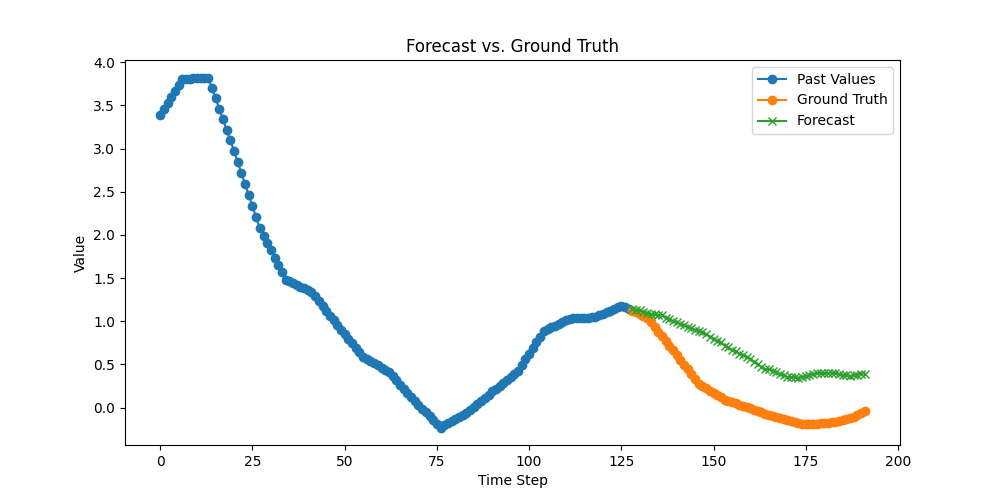
\includegraphics[width=\textwidth]{figures/time-moe/Germany_128_64.png}
          \caption{Healthcare - Horizon 128$\to$64}
     \end{subfigure}
     \begin{subfigure}[b]{0.32\textwidth}
          \centering
          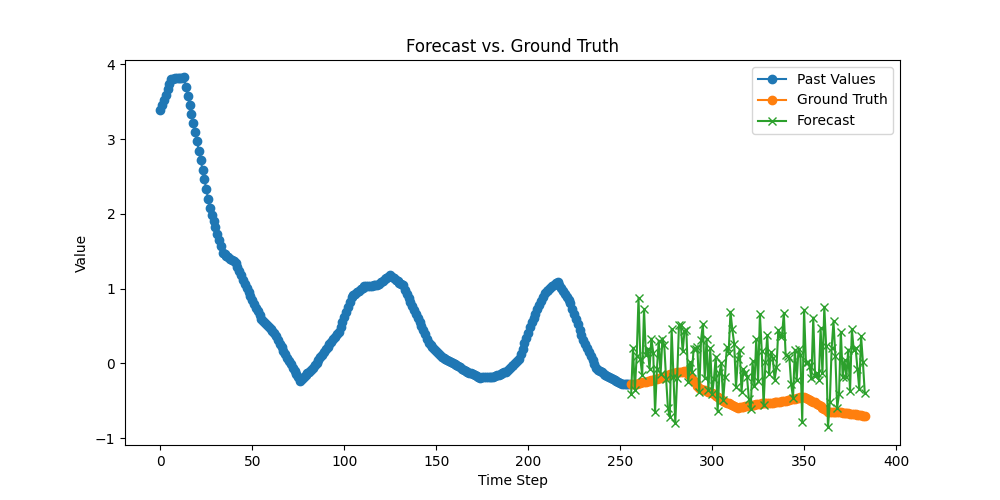
\includegraphics[width=\textwidth]{figures/time-moe/Germany_256_128.png}
          \caption{Healthcare - Horizon 256$\to$128}
     \end{subfigure}
     \caption{Time-MoE predictions on Healthcare dataset.}
 \end{figure}

\section{Regressors}

%---------------------------------------------------------
\subsection{Linear Regression}

\subsubsection{Weather Dataset}
\begin{figure}[h!]
    \centering
    \begin{subfigure}[b]{0.32\textwidth}
         \centering
         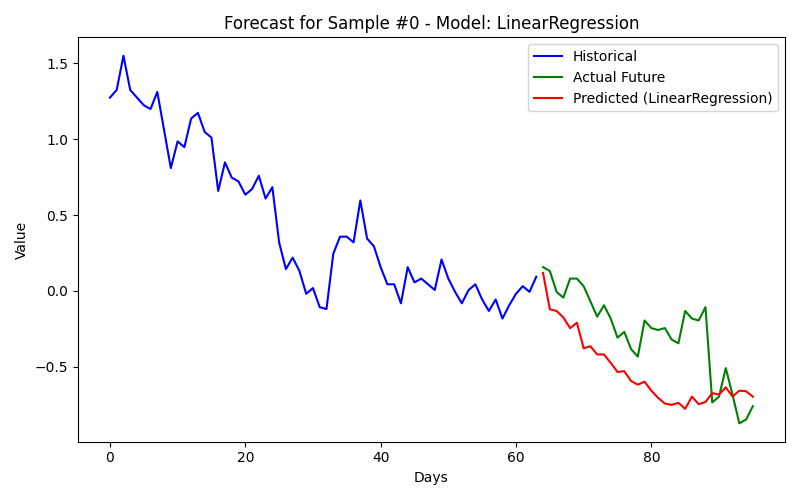
\includegraphics[width=\textwidth]{figures/regressors/LinearRegression/weather_64-32.png}
         \caption{Horizon 64$\to$32}
         \label{fig:LR_weather_64to32}
    \end{subfigure}
    \begin{subfigure}[b]{0.32\textwidth}
         \centering
         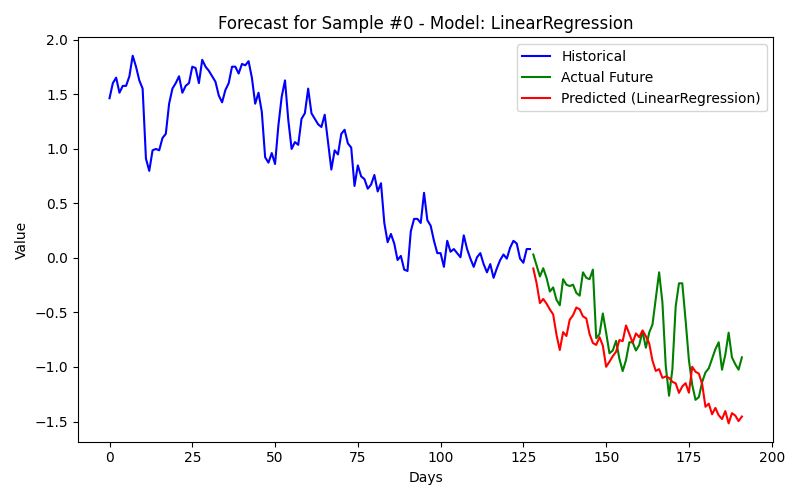
\includegraphics[width=\textwidth]{figures/regressors/LinearRegression/weather_128-64.png}
         \caption{Horizon 128$\to$64}
         \label{fig:LR_weather_128to64}
    \end{subfigure}
    \begin{subfigure}[b]{0.32\textwidth}
         \centering
         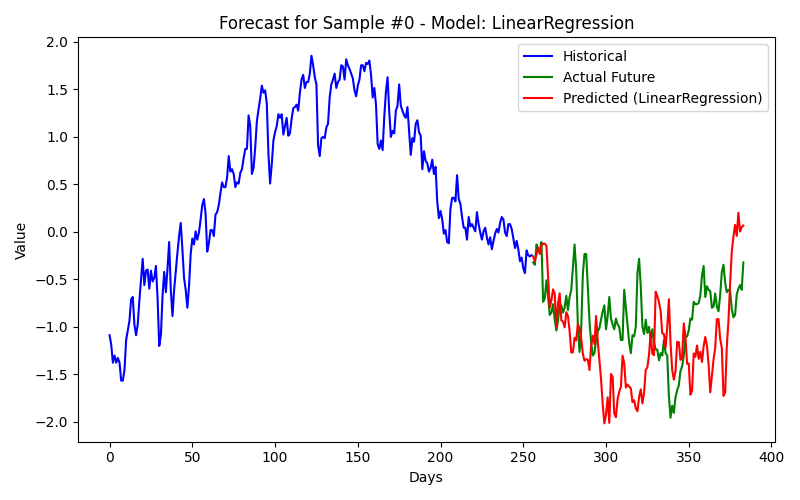
\includegraphics[width=\textwidth]{figures/regressors/LinearRegression/weather_256-128.png}
         \caption{Horizon 256$\to$128}
         \label{fig:LR_weather_256to128}
    \end{subfigure}
    \caption{Linear Regression forecasts on the Weather dataset for different horizons.}
    \label{fig:LR_weather_all}
\end{figure}

\subsubsection{Finance Dataset}
\begin{figure}[h!]
    \centering
    \begin{subfigure}[b]{0.32\textwidth}
         \centering
         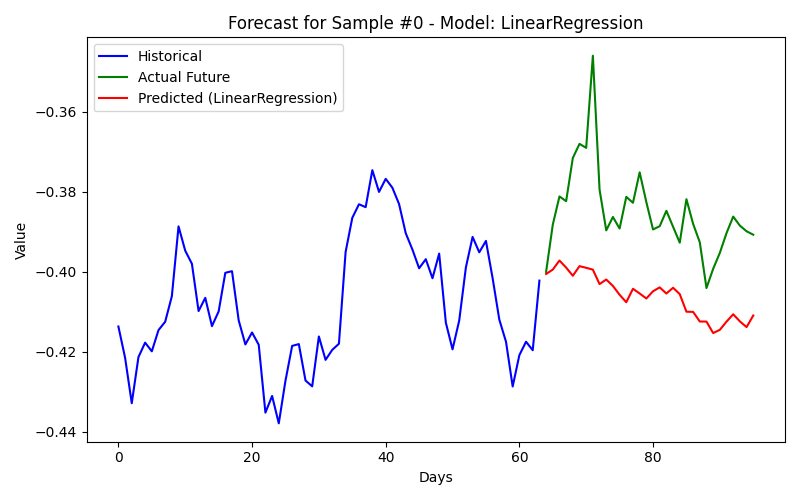
\includegraphics[width=\textwidth]{figures/regressors/LinearRegression/finance_64-32.png}
         \caption{Horizon 64$\to$32}
         \label{fig:LR_finance_64to32}
    \end{subfigure}
    \begin{subfigure}[b]{0.32\textwidth}
         \centering
         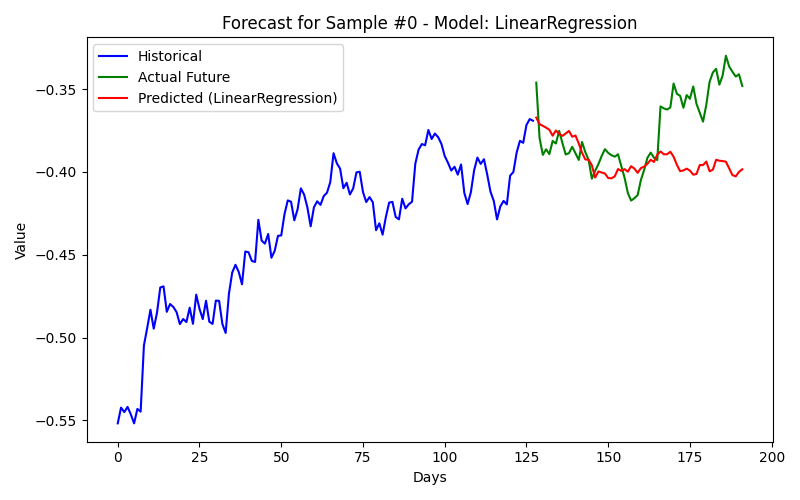
\includegraphics[width=\textwidth]{figures/regressors/LinearRegression/finance_128-64.png}
         \caption{Horizon 128$\to$64}
         \label{fig:LR_finance_128to64}
    \end{subfigure}
    \begin{subfigure}[b]{0.32\textwidth}
         \centering
         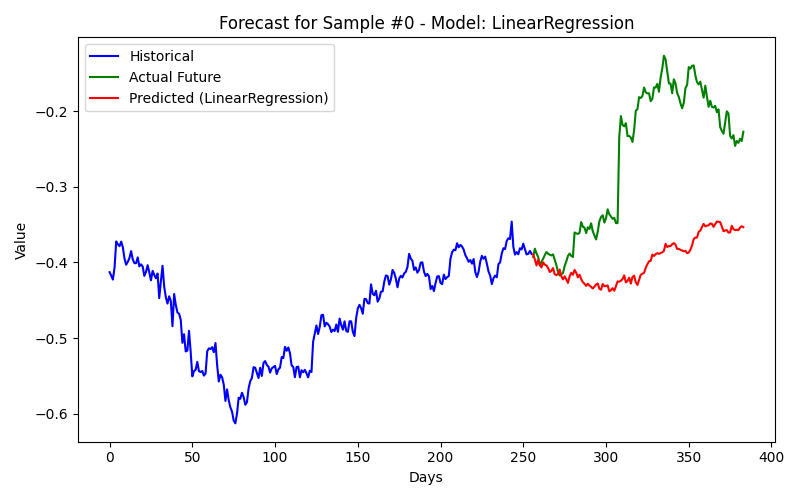
\includegraphics[width=\textwidth]{figures/regressors/LinearRegression/finance_256-128.png}
         \caption{Horizon 256$\to$128}
         \label{fig:LR_finance_256to128}
    \end{subfigure}
    \caption{Linear Regression forecasts on the Finance dataset for different horizons.}
    \label{fig:LR_finance_all}
\end{figure}

\subsubsection{Energy Dataset}
\begin{figure}[h!]
    \centering
    \begin{subfigure}[b]{0.32\textwidth}
         \centering
         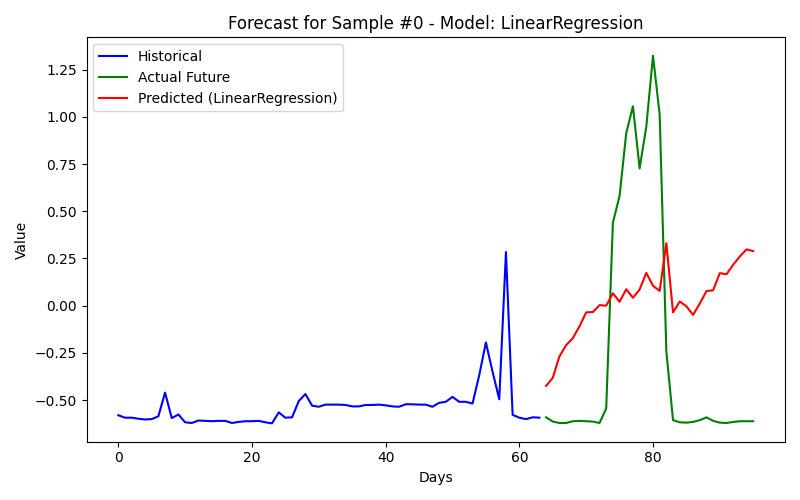
\includegraphics[width=\textwidth]{figures/regressors/LinearRegression/energy_64-32.png}
         \caption{Horizon 64$\to$32}
         \label{fig:LR_energy_64to32}
    \end{subfigure}
    \begin{subfigure}[b]{0.32\textwidth}
         \centering
         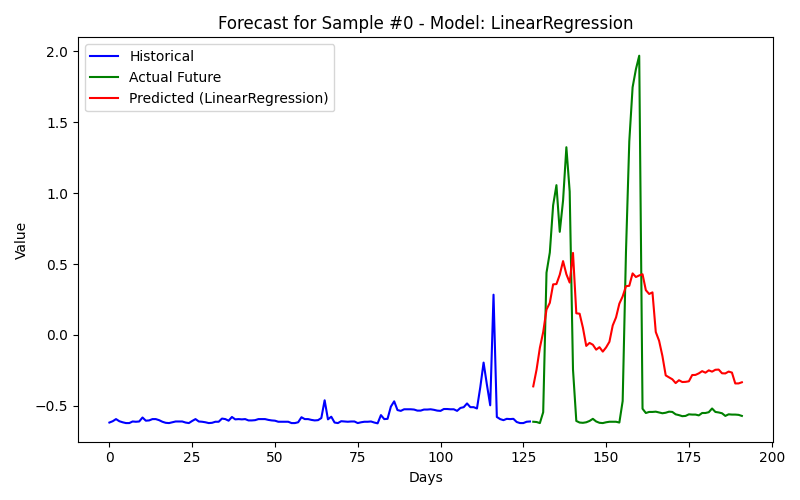
\includegraphics[width=\textwidth]{figures/regressors/LinearRegression/energy_128-64.png}
         \caption{Horizon 128$\to$64}
         \label{fig:LR_energy_128to64}
    \end{subfigure}
    \begin{subfigure}[b]{0.32\textwidth}
         \centering
         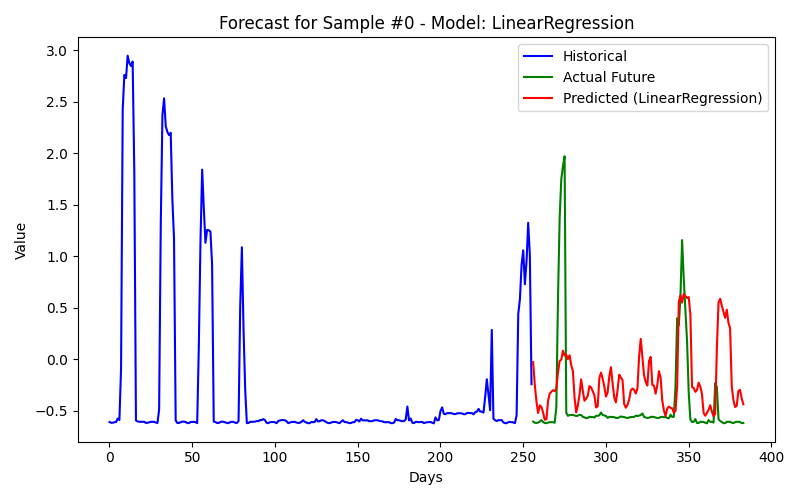
\includegraphics[width=\textwidth]{figures/regressors/LinearRegression/energy_256-128.png}
         \caption{Horizon 256$\to$128}
         \label{fig:LR_energy_256to128}
    \end{subfigure}
    \caption{Linear Regression forecasts on the Energy dataset for different horizons.}
    \label{fig:LR_energy_all}
\end{figure}

\subsubsection{Healthcare Dataset}
\begin{figure}[h!]
    \centering
    \begin{subfigure}[b]{0.32\textwidth}
         \centering
         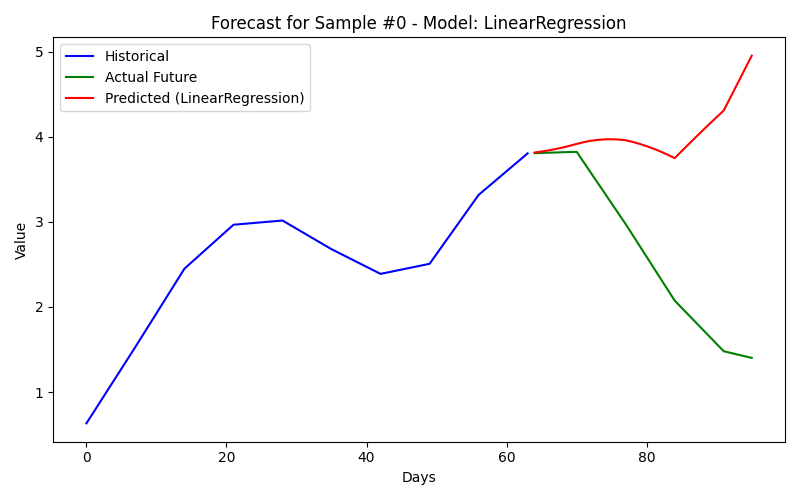
\includegraphics[width=\textwidth]{figures/regressors/LinearRegression/healthcare_64-32.png}
         \caption{Horizon 64$\to$32}
         \label{fig:LR_healthcare_64to32}
    \end{subfigure}
    \begin{subfigure}[b]{0.32\textwidth}
         \centering
         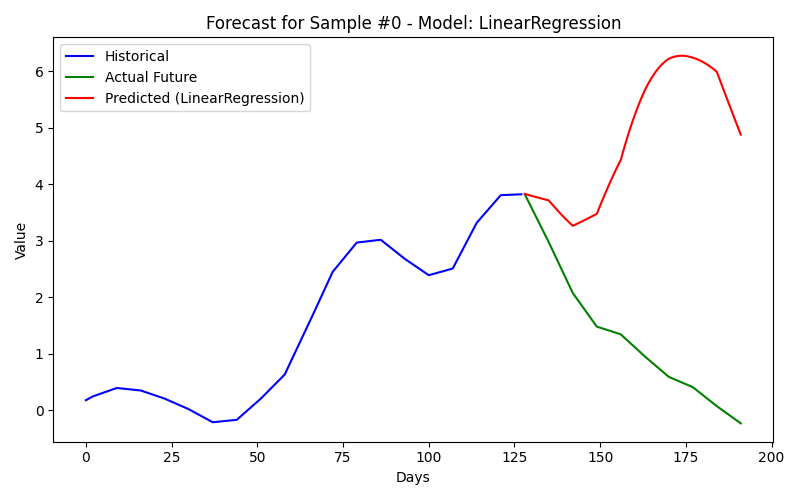
\includegraphics[width=\textwidth]{figures/regressors/LinearRegression/healthcare_128-64.png}
         \caption{Horizon 128$\to$64}
         \label{fig:LR_healthcare_128to64}
    \end{subfigure}
    \begin{subfigure}[b]{0.32\textwidth}
         \centering
         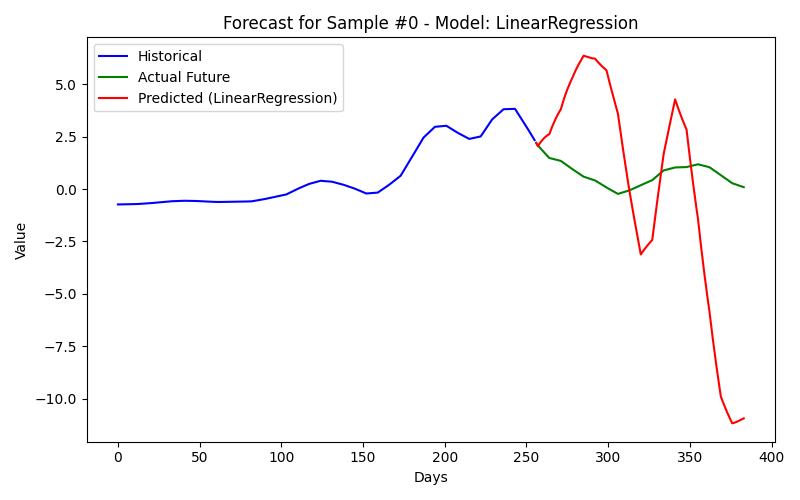
\includegraphics[width=\textwidth]{figures/regressors/LinearRegression/healthcare_256-128.png}
         \caption{Horizon 256$\to$128}
         \label{fig:LR_healthcare_256to128}
    \end{subfigure}
    \caption{Linear Regression forecasts on the Healthcare dataset for different horizons.}
    \label{fig:LR_healthcare_all}
\end{figure}

\newpage
%---------------------------------------------------------
\subsection{Random Forest Regressor}

\subsubsection{Weather Dataset}
\begin{figure}[h!]
    \centering
    \begin{subfigure}[b]{0.32\textwidth}
         \centering
         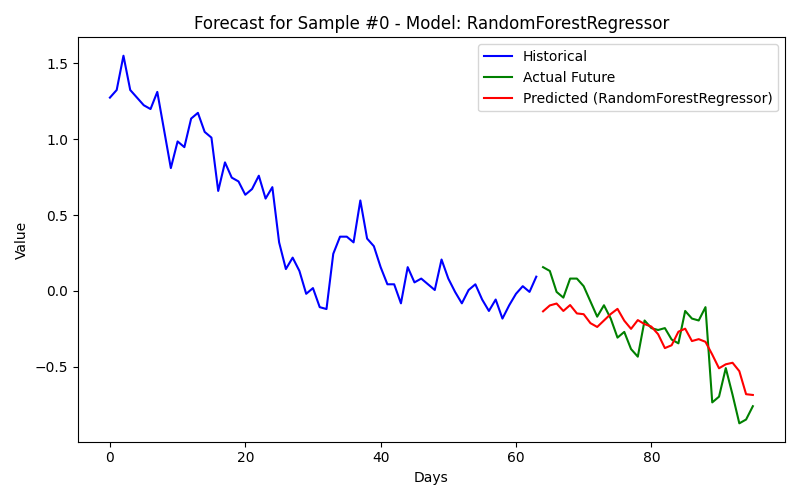
\includegraphics[width=\textwidth]{figures/regressors/RandomForestRegressor/weather_64-32.png}
         \caption{Horizon 64$\to$32}
         \label{fig:RF_weather_64to32}
    \end{subfigure}
    \begin{subfigure}[b]{0.32\textwidth}
         \centering
         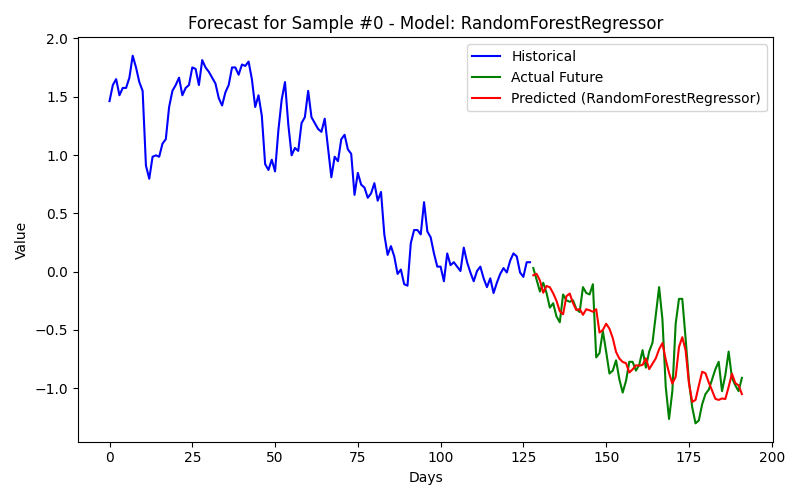
\includegraphics[width=\textwidth]{figures/regressors/RandomForestRegressor/weather_128-64.png}
         \caption{Horizon 128$\to$64}
         \label{fig:RF_weather_128to64}
    \end{subfigure}
    \begin{subfigure}[b]{0.32\textwidth}
         \centering
         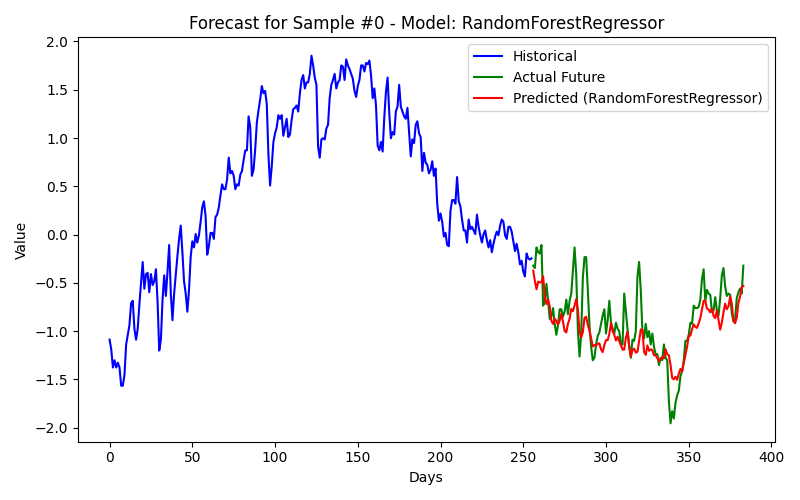
\includegraphics[width=\textwidth]{figures/regressors/RandomForestRegressor/weather_256-128.png}
         \caption{Horizon 256$\to$128}
         \label{fig:RF_weather_256to128}
    \end{subfigure}
    \caption{Random Forest forecasts on the Weather dataset for different horizons.}
    \label{fig:RF_weather_all}
\end{figure}

\subsubsection{Finance Dataset}
\begin{figure}[h!]
    \centering
    \begin{subfigure}[b]{0.32\textwidth}
         \centering
         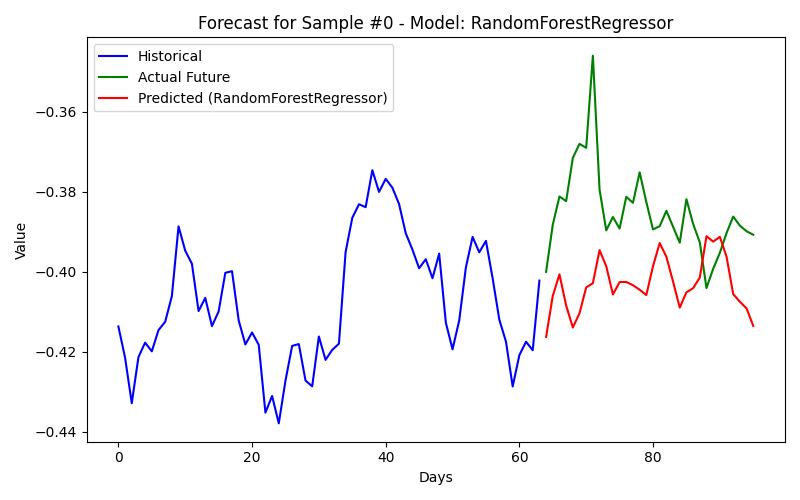
\includegraphics[width=\textwidth]{figures/regressors/RandomForestRegressor/finance_64-32.png}
         \caption{Horizon 64$\to$32}
         \label{fig:RF_finance_64to32}
    \end{subfigure}
    \begin{subfigure}[b]{0.32\textwidth}
         \centering
         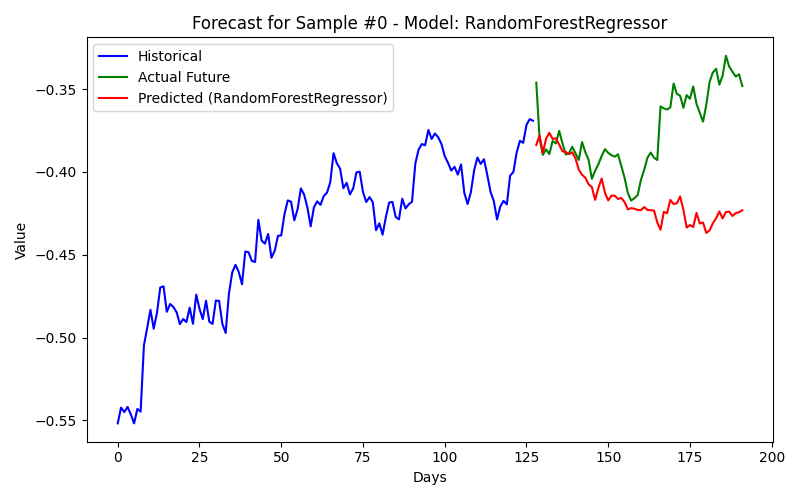
\includegraphics[width=\textwidth]{figures/regressors/RandomForestRegressor/finance_128-64.png}
         \caption{Horizon 128$\to$64}
         \label{fig:RF_finance_128to64}
    \end{subfigure}
    \begin{subfigure}[b]{0.32\textwidth}
         \centering
         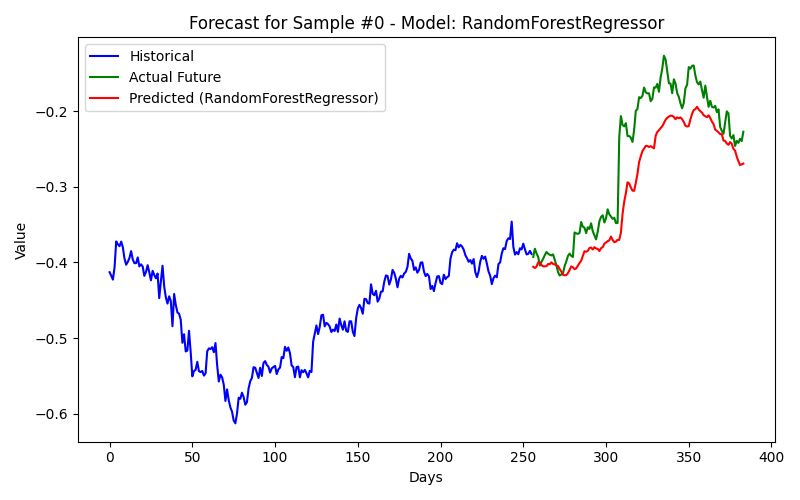
\includegraphics[width=\textwidth]{figures/regressors/RandomForestRegressor/finance_256-128.png}
         \caption{Horizon 256$\to$128}
         \label{fig:RF_finance_256to128}
    \end{subfigure}
    \caption{Random Forest forecasts on the Finance dataset for different horizons.}
    \label{fig:RF_finance_all}
\end{figure}

\subsubsection{Energy Dataset}
\begin{figure}[h!]
    \centering
    \begin{subfigure}[b]{0.32\textwidth}
         \centering
         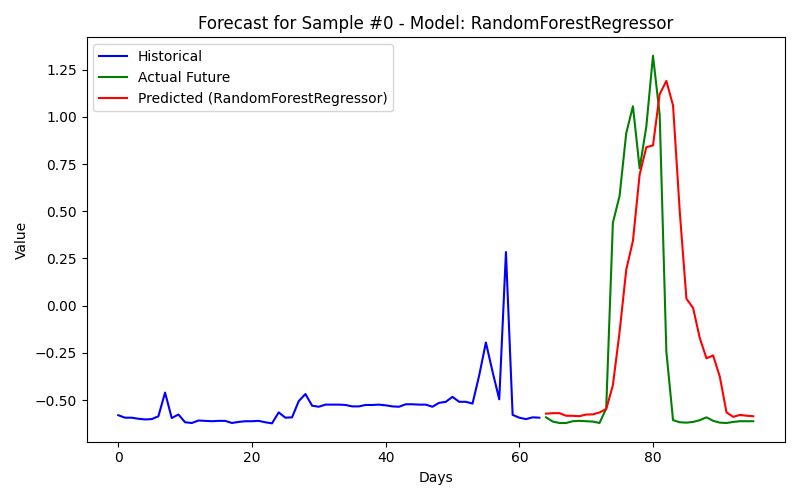
\includegraphics[width=\textwidth]{figures/regressors/RandomForestRegressor/energy_64-32.png}
         \caption{Horizon 64$\to$32}
         \label{fig:RF_energy_64to32}
    \end{subfigure}
    \begin{subfigure}[b]{0.32\textwidth}
         \centering
         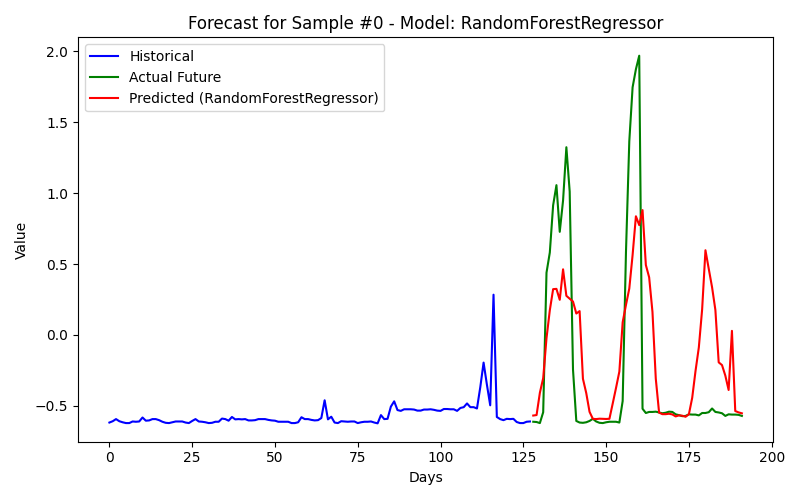
\includegraphics[width=\textwidth]{figures/regressors/RandomForestRegressor/energy_128-64.png}
         \caption{Horizon 128$\to$64}
         \label{fig:RF_energy_128to64}
    \end{subfigure}
    \begin{subfigure}[b]{0.32\textwidth}
         \centering
         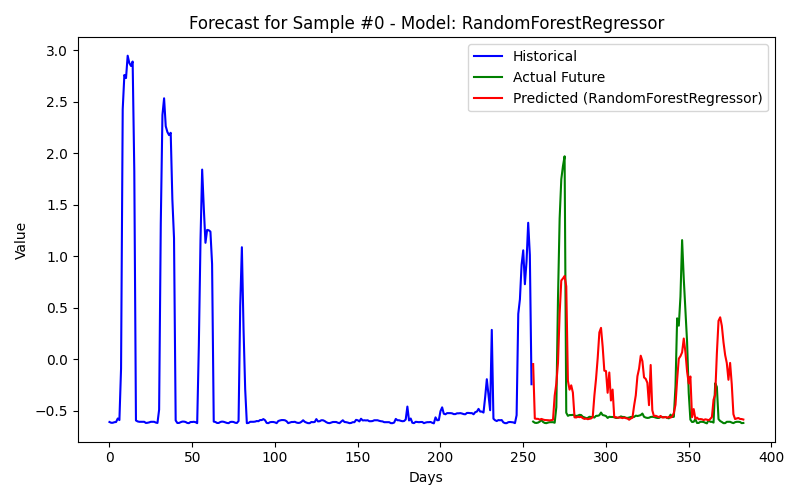
\includegraphics[width=\textwidth]{figures/regressors/RandomForestRegressor/energy_256-128.png}
         \caption{Horizon 256$\to$128}
         \label{fig:RF_energy_256to128}
    \end{subfigure}
    \caption{Random Forest forecasts on the Energy dataset for different horizons.}
    \label{fig:RF_energy_all}
\end{figure}

\subsubsection{Healthcare Dataset}
\begin{figure}[h!]
    \centering
    \begin{subfigure}[b]{0.32\textwidth}
         \centering
         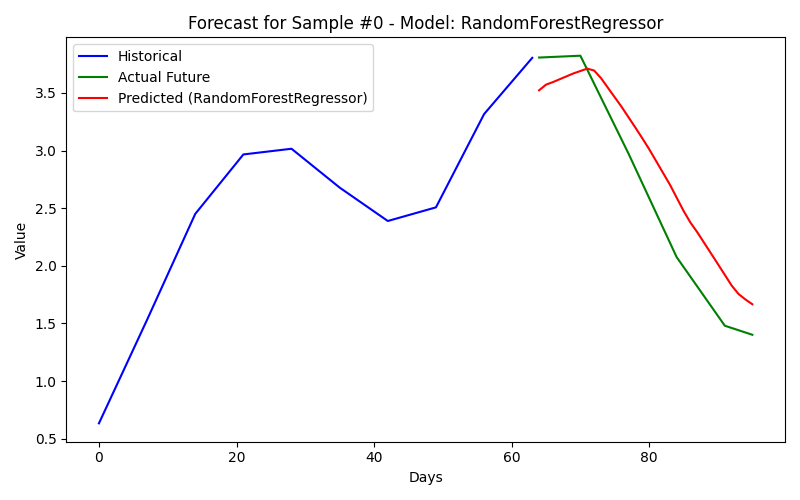
\includegraphics[width=\textwidth]{figures/regressors/RandomForestRegressor/healthcare_64-32.png}
         \caption{Horizon 64$\to$32}
         \label{fig:RF_healthcare_64to32}
    \end{subfigure}
    \begin{subfigure}[b]{0.32\textwidth}
         \centering
         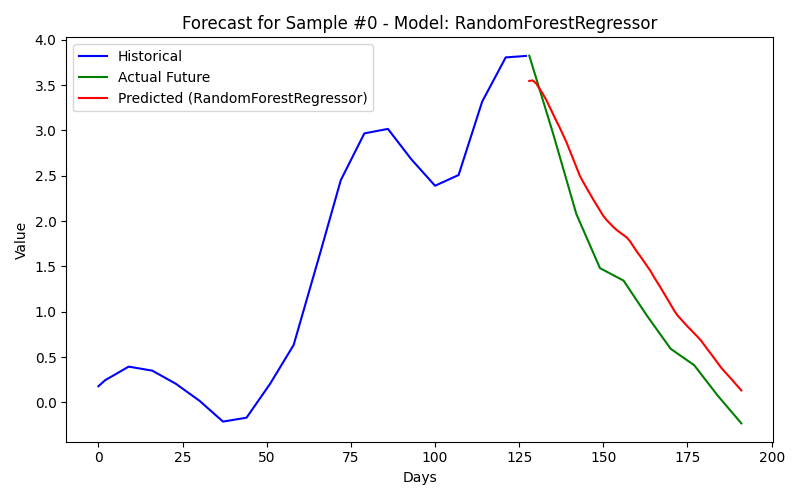
\includegraphics[width=\textwidth]{figures/regressors/RandomForestRegressor/healthcare_128-64.png}
         \caption{Horizon 128$\to$64}
         \label{fig:RF_healthcare_128to64}
    \end{subfigure}
    \begin{subfigure}[b]{0.32\textwidth}
         \centering
         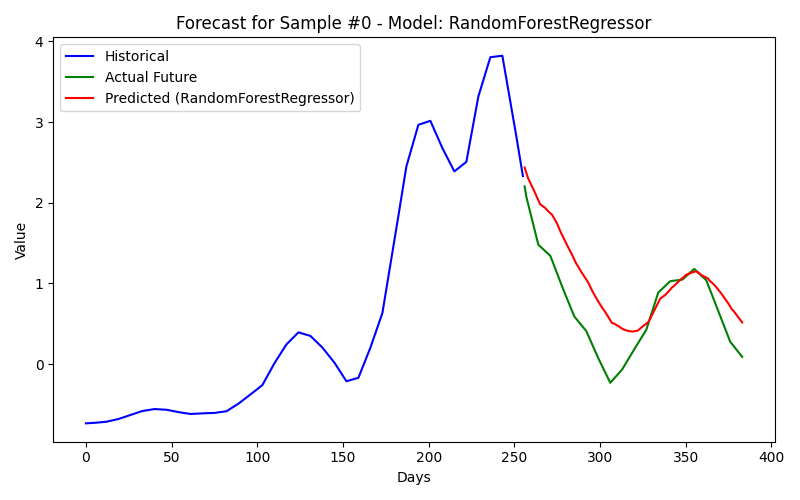
\includegraphics[width=\textwidth]{figures/regressors/RandomForestRegressor/healthcare_256-128.png}
         \caption{Horizon 256$\to$128}
         \label{fig:RF_healthcare_256to128}
    \end{subfigure}
    \caption{Random Forest forecasts on the Healthcare dataset for different horizons.}
    \label{fig:RF_healthcare_all}
\end{figure}

\newpage
%---------------------------------------------------------
\subsection{Extra Trees Regressor}

\subsubsection{Weather Dataset}
\begin{figure}[h!]
    \centering
    \begin{subfigure}[b]{0.32\textwidth}
         \centering
         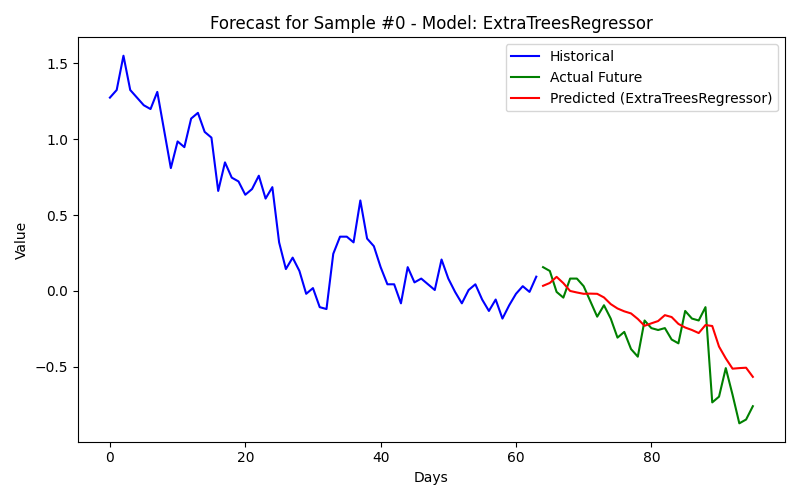
\includegraphics[width=\textwidth]{figures/regressors/ExtraTreesRegressor/weather_64-32.png}
         \caption{Horizon 64$\to$32}
         \label{fig:ET_weather_64to32}
    \end{subfigure}
    \begin{subfigure}[b]{0.32\textwidth}
         \centering
         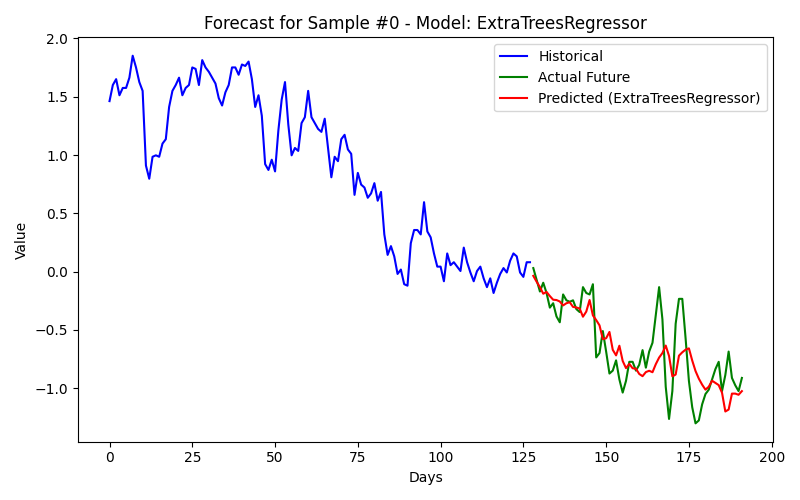
\includegraphics[width=\textwidth]{figures/regressors/ExtraTreesRegressor/weather_128-64.png}
         \caption{Horizon 128$\to$64}
         \label{fig:ET_weather_128to64}
    \end{subfigure}
    \begin{subfigure}[b]{0.32\textwidth}
         \centering
         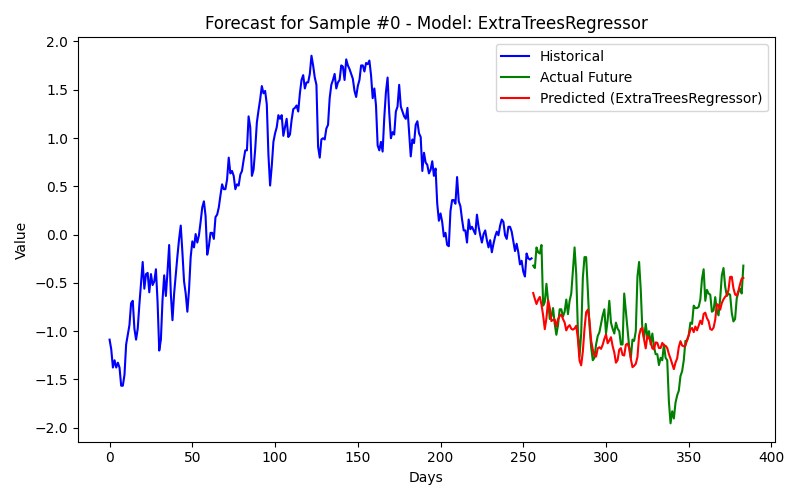
\includegraphics[width=\textwidth]{figures/regressors/ExtraTreesRegressor/weather_256-128.png}
         \caption{Horizon 256$\to$128}
         \label{fig:ET_weather_256to128}
    \end{subfigure}
    \caption{Extra Trees forecasts on the Weather dataset for different horizons.}
    \label{fig:ET_weather_all}
\end{figure}

\subsubsection{Finance Dataset}
\begin{figure}[h!]
    \centering
    \begin{subfigure}[b]{0.32\textwidth}
         \centering
         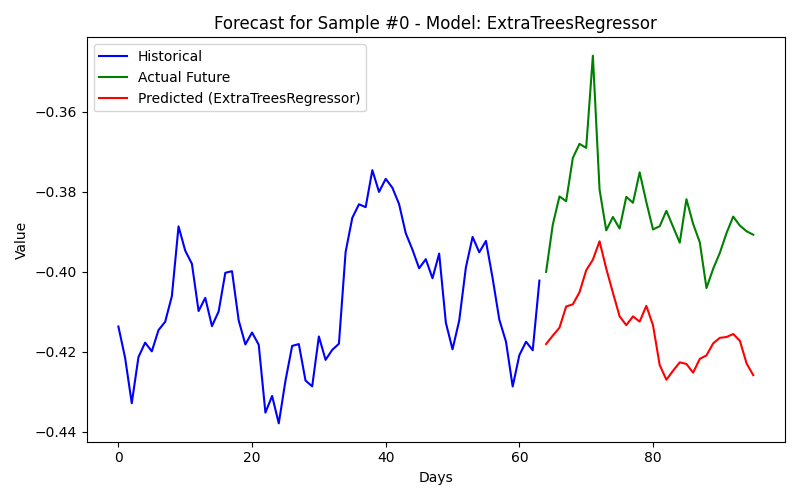
\includegraphics[width=\textwidth]{figures/regressors/ExtraTreesRegressor/finance_64-32.png}
         \caption{Horizon 64$\to$32}
         \label{fig:ET_finance_64to32}
    \end{subfigure}
    \begin{subfigure}[b]{0.32\textwidth}
         \centering
         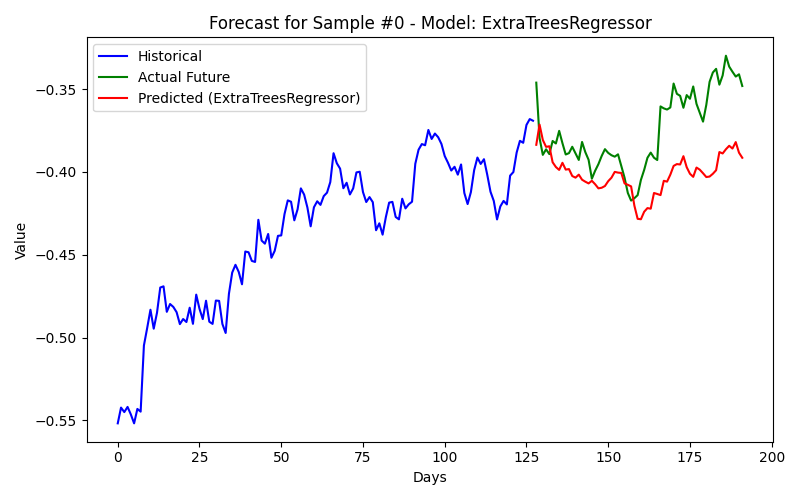
\includegraphics[width=\textwidth]{figures/regressors/ExtraTreesRegressor/finance_128-64.png}
         \caption{Horizon 128$\to$64}
         \label{fig:ET_finance_128to64}
    \end{subfigure}
    \begin{subfigure}[b]{0.32\textwidth}
         \centering
         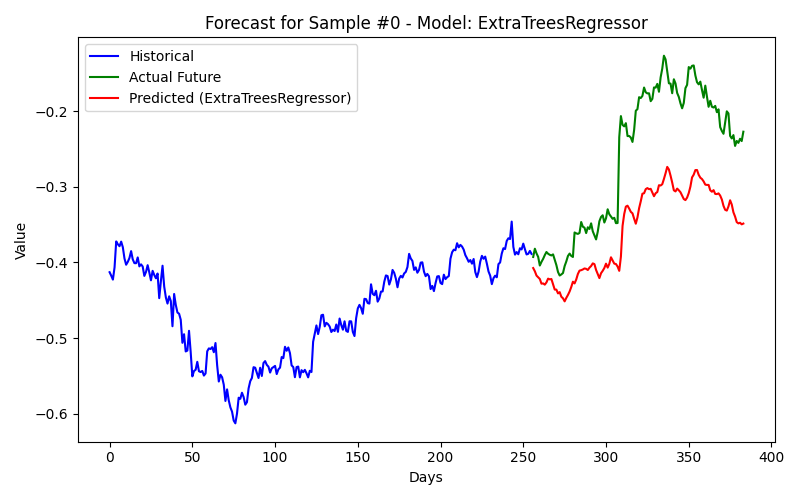
\includegraphics[width=\textwidth]{figures/regressors/ExtraTreesRegressor/finance_256-128.png}
         \caption{Horizon 256$\to$128}
         \label{fig:ET_finance_256to128}
    \end{subfigure}
    \caption{Extra Trees forecasts on the Finance dataset for different horizons.}
    \label{fig:ET_finance_all}
\end{figure}

\subsubsection{Energy Dataset}
\begin{figure}[h!]
    \centering
    \begin{subfigure}[b]{0.32\textwidth}
         \centering
         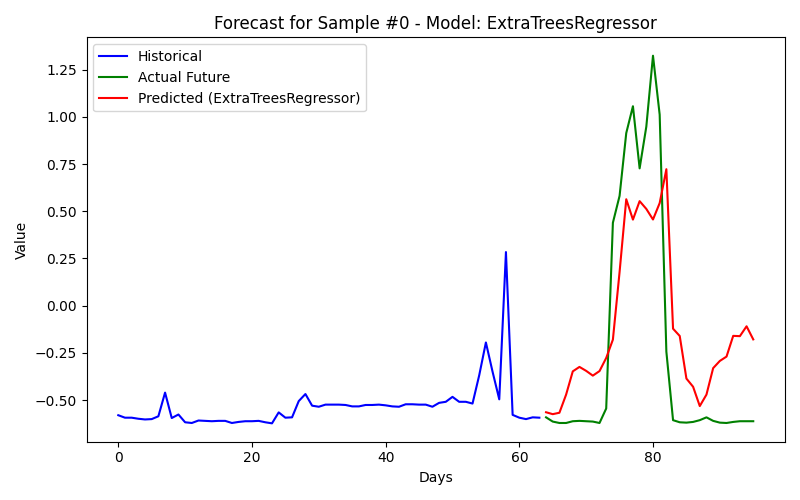
\includegraphics[width=\textwidth]{figures/regressors/ExtraTreesRegressor/energy_64-32.png}
         \caption{Horizon 64$\to$32}
         \label{fig:ET_energy_64to32}
    \end{subfigure}
    \begin{subfigure}[b]{0.32\textwidth}
         \centering
         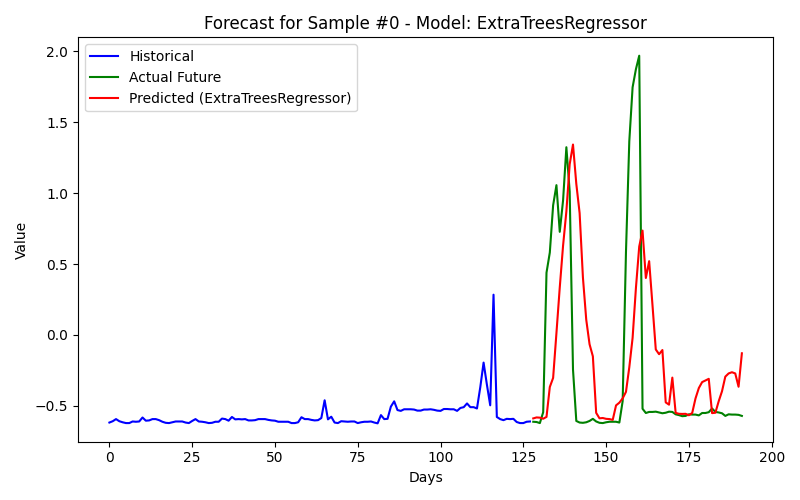
\includegraphics[width=\textwidth]{figures/regressors/ExtraTreesRegressor/energy_128-64.png}
         \caption{Horizon 128$\to$64}
         \label{fig:ET_energy_128to64}
    \end{subfigure}
    \begin{subfigure}[b]{0.32\textwidth}
         \centering
         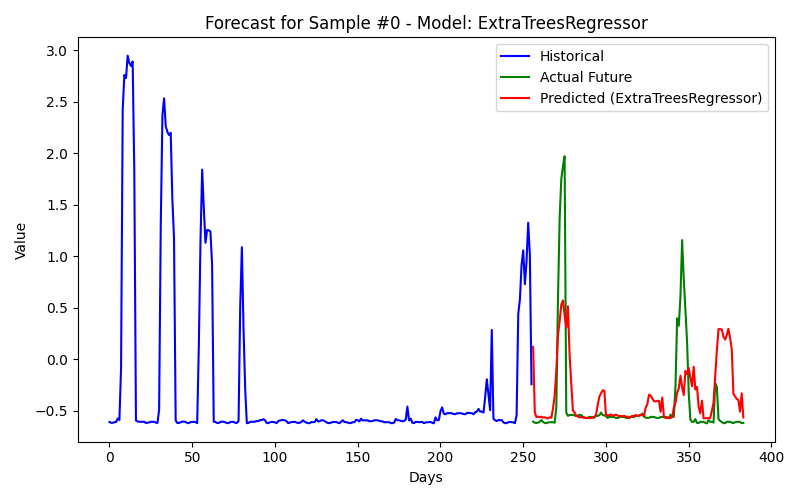
\includegraphics[width=\textwidth]{figures/regressors/ExtraTreesRegressor/energy_256-128.png}
         \caption{Horizon 256$\to$128}
         \label{fig:ET_energy_256to128}
    \end{subfigure}
    \caption{Extra Trees forecasts on the Energy dataset for different horizons.}
    \label{fig:ET_energy_all}
\end{figure}

\subsubsection{Healthcare Dataset}
\begin{figure}[h!]
    \centering
    \begin{subfigure}[b]{0.32\textwidth}
         \centering
         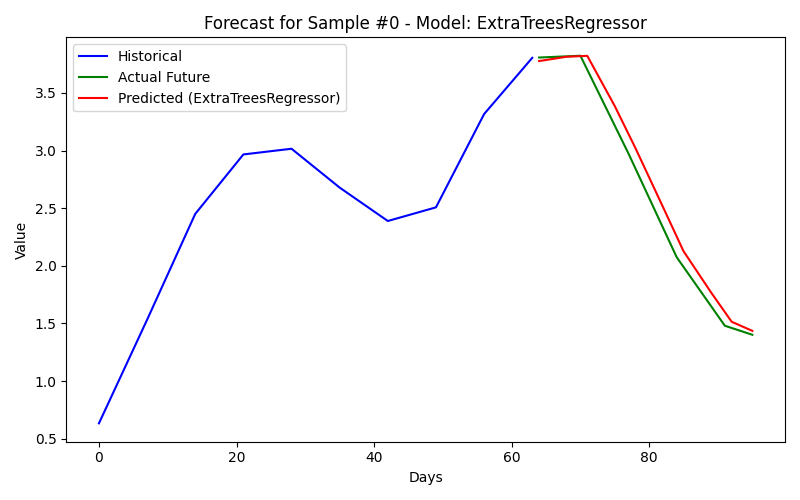
\includegraphics[width=\textwidth]{figures/regressors/ExtraTreesRegressor/healthcare_64-32.png}
         \caption{Horizon 64$\to$32}
         \label{fig:ET_healthcare_64to32}
    \end{subfigure}
    \begin{subfigure}[b]{0.32\textwidth}
         \centering
         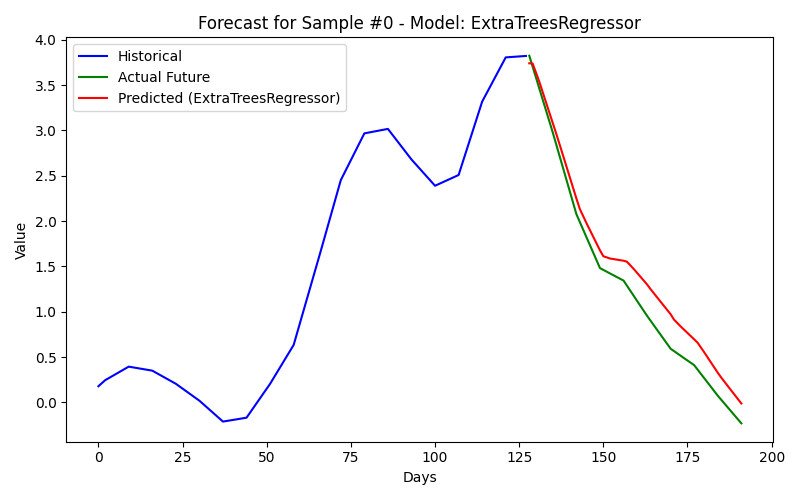
\includegraphics[width=\textwidth]{figures/regressors/ExtraTreesRegressor/healthcare_128-64.png}
         \caption{Horizon 128$\to$64}
         \label{fig:ET_healthcare_128to64}
    \end{subfigure}
    \begin{subfigure}[b]{0.32\textwidth}
         \centering
         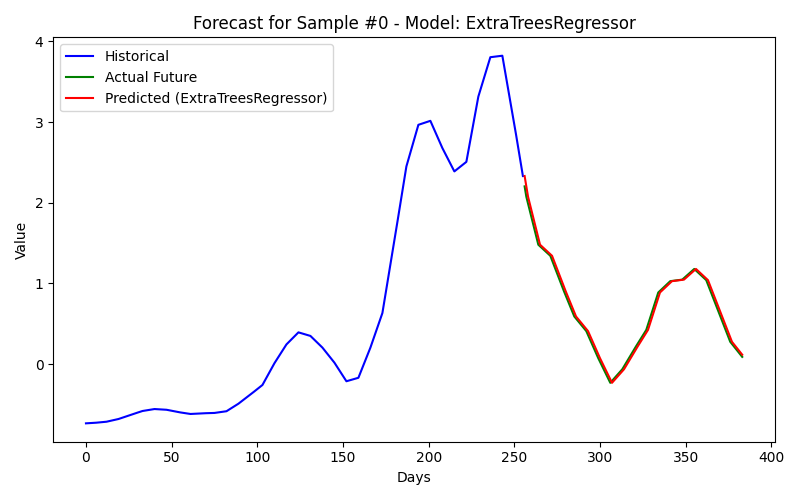
\includegraphics[width=\textwidth]{figures/regressors/ExtraTreesRegressor/healthcare_256-128.png}
         \caption{Horizon 256$\to$128}
         \label{fig:ET_healthcare_256to128}
    \end{subfigure}
    \caption{Extra Trees forecasts on the Healthcare dataset for different horizons.}
    \label{fig:ET_healthcare_all}
\end{figure}

\newpage
%---------------------------------------------------------
\subsection{MLP Regressor}

\subsubsection{Weather Dataset}
\begin{figure}[h!]
    \centering
    \begin{subfigure}[b]{0.32\textwidth}
         \centering
         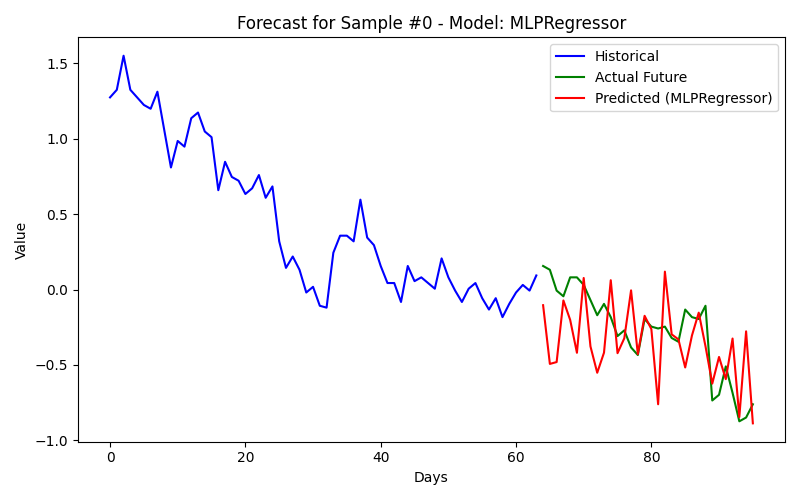
\includegraphics[width=\textwidth]{figures/regressors/MLPRegressor/weather_64-32.png}
         \caption{Horizon 64$\to$32}
         \label{fig:MLP_weather_64to32}
    \end{subfigure}
    \begin{subfigure}[b]{0.32\textwidth}
         \centering
         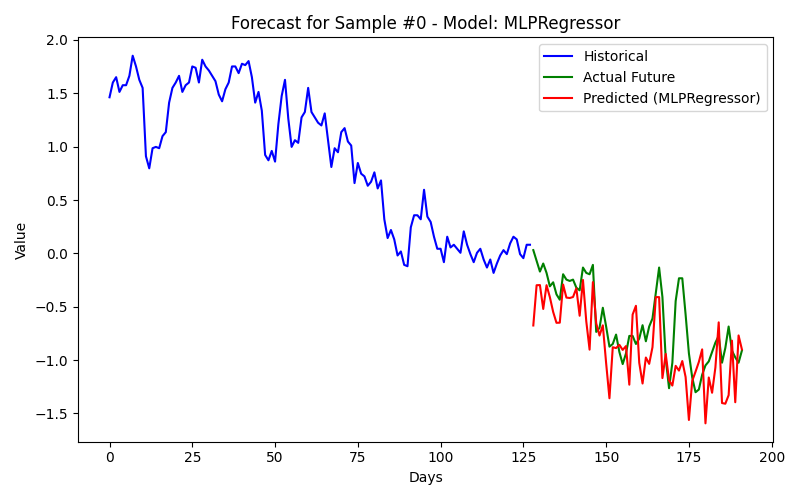
\includegraphics[width=\textwidth]{figures/regressors/MLPRegressor/weather_128-64.png}
         \caption{Horizon 128$\to$64}
         \label{fig:MLP_weather_128to64}
    \end{subfigure}
    \begin{subfigure}[b]{0.32\textwidth}
         \centering
         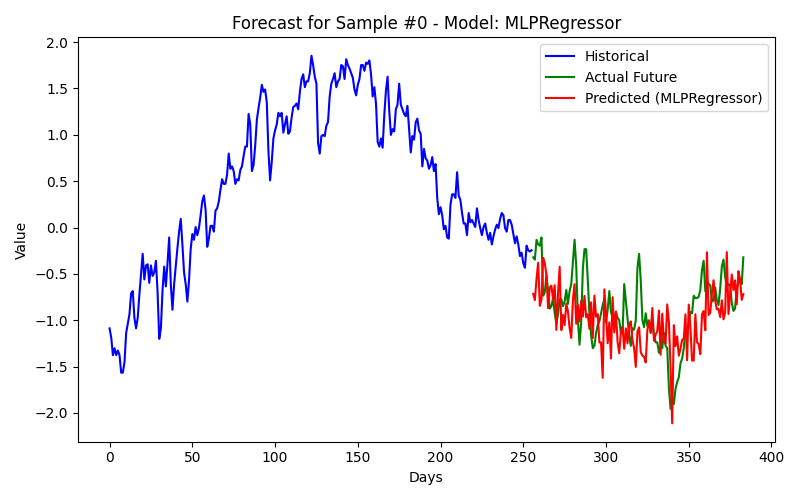
\includegraphics[width=\textwidth]{figures/regressors/MLPRegressor/weather_256-128.png}
         \caption{Horizon 256$\to$128}
         \label{fig:MLP_weather_256to128}
    \end{subfigure}
    \caption{MLP Regressor forecasts on the Weather dataset for different horizons.}
    \label{fig:MLP_weather_all}
\end{figure}

\subsubsection{Finance Dataset}
\begin{figure}[h!]
    \centering
    \begin{subfigure}[b]{0.32\textwidth}
         \centering
         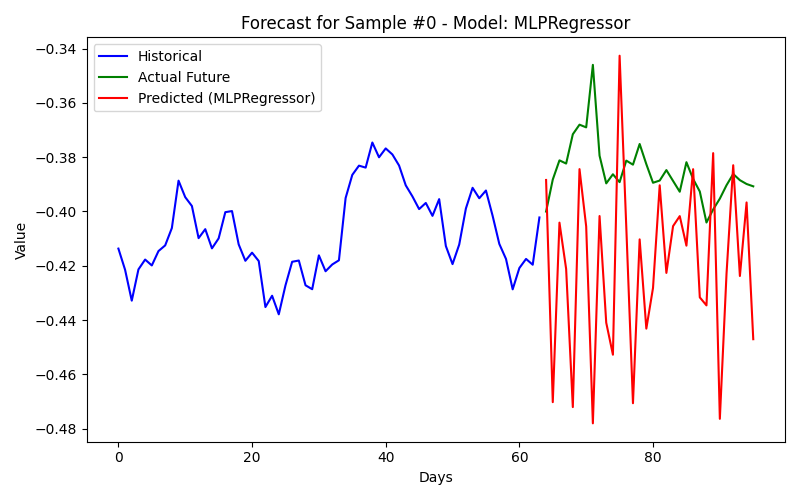
\includegraphics[width=\textwidth]{figures/regressors/MLPRegressor/finance_64-32.png}
         \caption{Horizon 64$\to$32}
         \label{fig:MLP_finance_64to32}
    \end{subfigure}
    \begin{subfigure}[b]{0.32\textwidth}
         \centering
         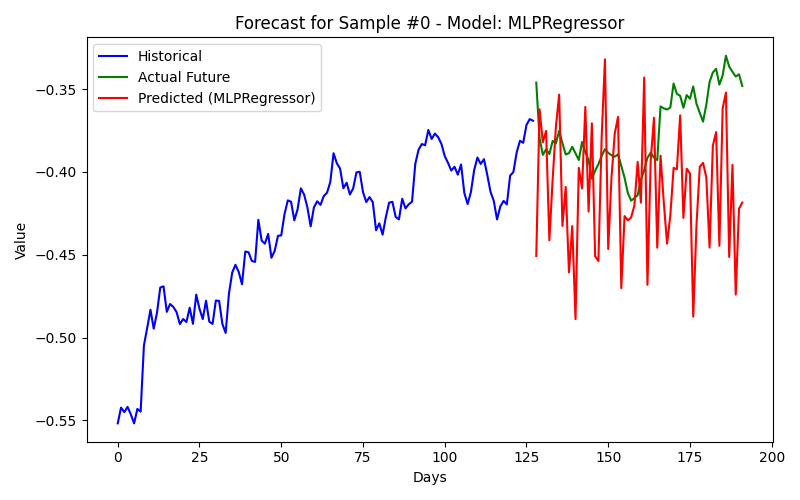
\includegraphics[width=\textwidth]{figures/regressors/MLPRegressor/finance_128-64.png}
         \caption{Horizon 128$\to$64}
         \label{fig:MLP_finance_128to64}
    \end{subfigure}
    \begin{subfigure}[b]{0.32\textwidth}
         \centering
         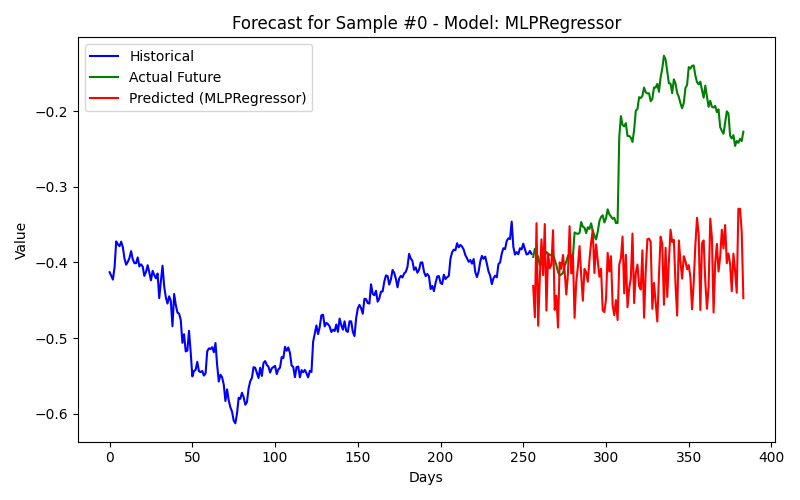
\includegraphics[width=\textwidth]{figures/regressors/MLPRegressor/finance_256-128.png}
         \caption{Horizon 256$\to$128}
         \label{fig:MLP_finance_256to128}
    \end{subfigure}
    \caption{MLP Regressor forecasts on the Finance dataset for different horizons.}
    \label{fig:MLP_finance_all}
\end{figure}

\subsubsection{Energy Dataset}
\begin{figure}[h!]
    \centering
    \begin{subfigure}[b]{0.32\textwidth}
         \centering
         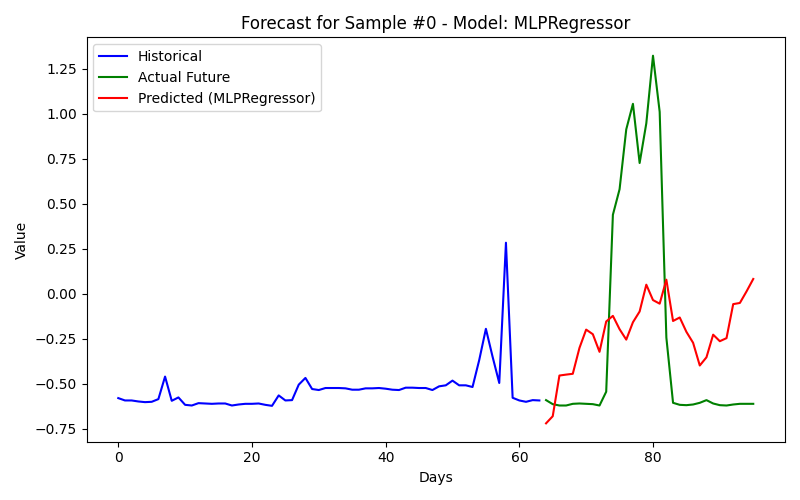
\includegraphics[width=\textwidth]{figures/regressors/MLPRegressor/energy_64-32.png}
         \caption{Horizon 64$\to$32}
         \label{fig:MLP_energy_64to32}
    \end{subfigure}
    \begin{subfigure}[b]{0.32\textwidth}
         \centering
         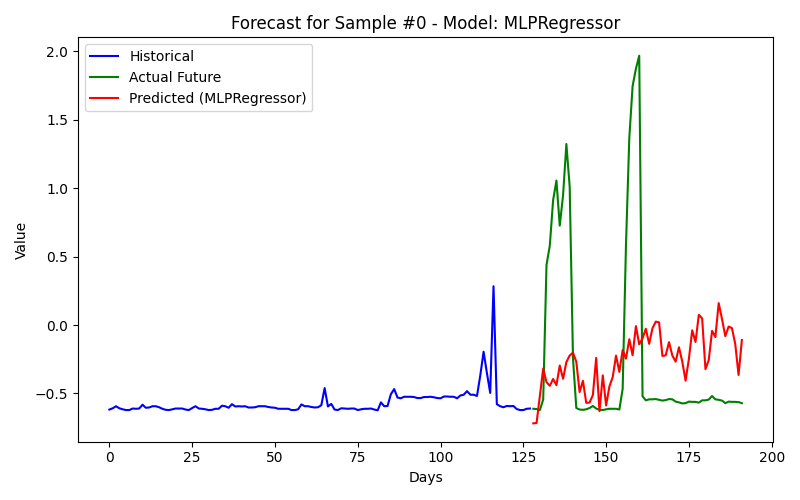
\includegraphics[width=\textwidth]{figures/regressors/MLPRegressor/energy_128-64.png}
         \caption{Horizon 128$\to$64}
         \label{fig:MLP_energy_128to64}
    \end{subfigure}
    \begin{subfigure}[b]{0.32\textwidth}
         \centering
         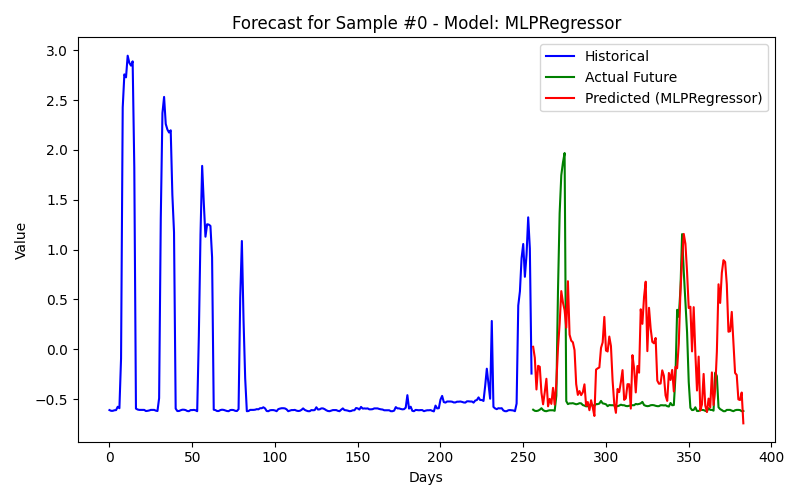
\includegraphics[width=\textwidth]{figures/regressors/MLPRegressor/energy_256-128.png}
         \caption{Horizon 256$\to$128}
         \label{fig:MLP_energy_256to128}
    \end{subfigure}
    \caption{MLP Regressor forecasts on the Energy dataset for different horizons.}
    \label{fig:MLP_energy_all}
\end{figure}

\subsubsection{Healthcare Dataset}
\begin{figure}[h!]
    \centering
    \begin{subfigure}[b]{0.32\textwidth}
         \centering
         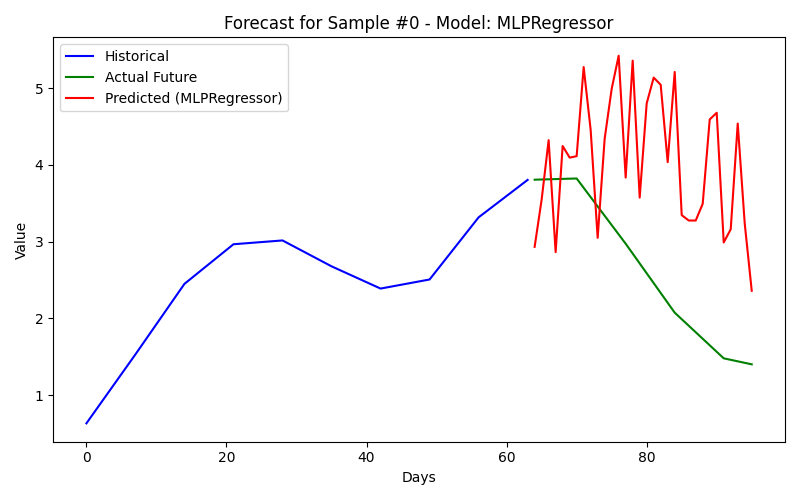
\includegraphics[width=\textwidth]{figures/regressors/MLPRegressor/healthcare_64-32.png}
         \caption{Horizon 64$\to$32}
         \label{fig:MLP_healthcare_64to32}
    \end{subfigure}
    \begin{subfigure}[b]{0.32\textwidth}
         \centering
         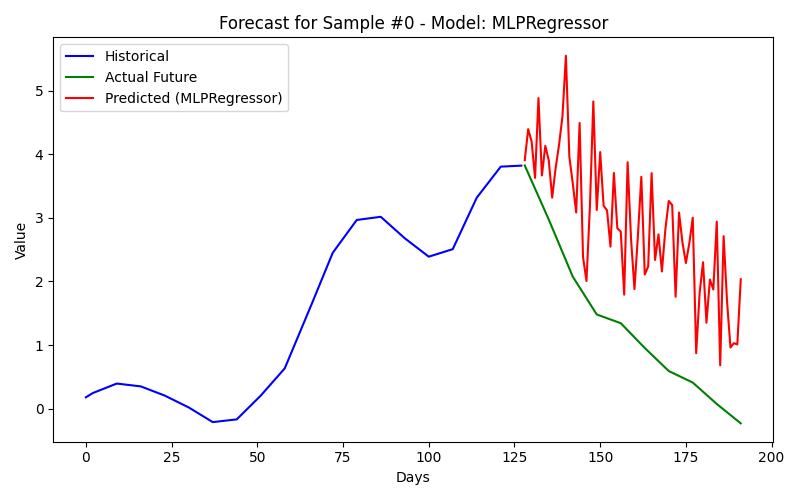
\includegraphics[width=\textwidth]{figures/regressors/MLPRegressor/healthcare_128-64.png}
         \caption{Horizon 128$\to$64}
         \label{fig:MLP_healthcare_128to64}
    \end{subfigure}
    \begin{subfigure}[b]{0.32\textwidth}
         \centering
         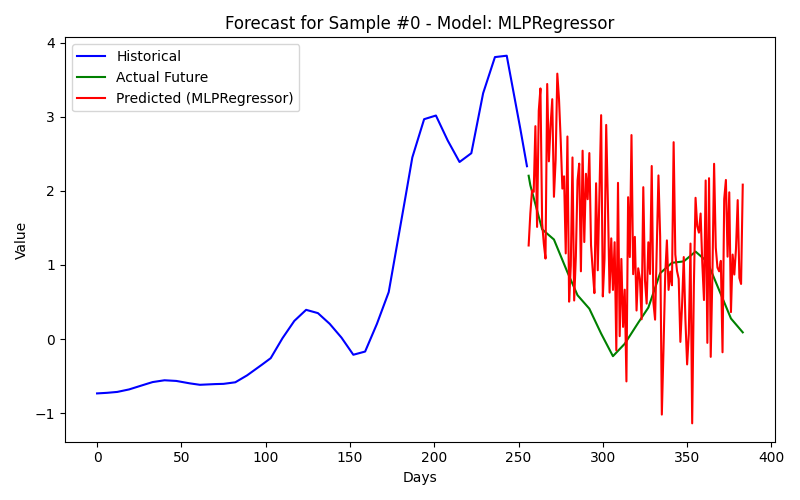
\includegraphics[width=\textwidth]{figures/regressors/MLPRegressor/healthcare_256-128.png}
         \caption{Horizon 256$\to$128}
         \label{fig:MLP_healthcare_256to128}
    \end{subfigure}
    \caption{MLP Regressor forecasts on the Healthcare dataset for different horizons.}
    \label{fig:MLP_healthcare_all}
\end{figure}

\newpage
%---------------------------------------------------------
\subsection{HistGradientBoosting Regressor}

\subsubsection{Weather Dataset}
\begin{figure}[h!]
    \centering
    \begin{subfigure}[b]{0.32\textwidth}
         \centering
         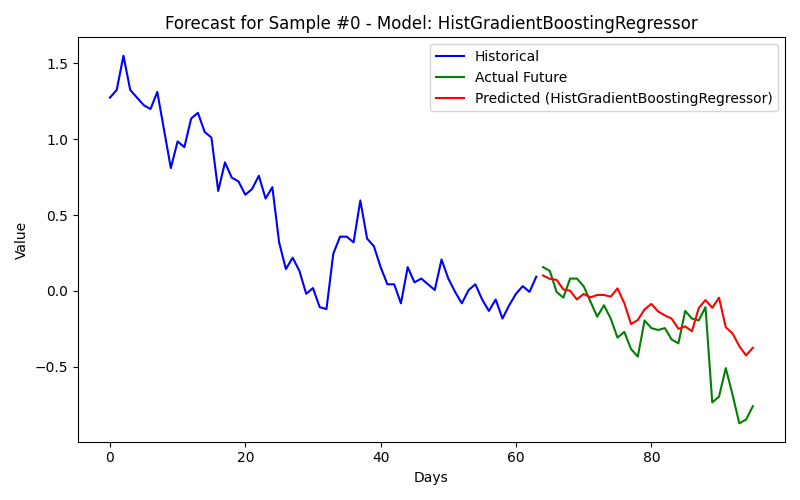
\includegraphics[width=\textwidth]{figures/regressors/HistGradientBoostingRegressor/weather_64-32.png}
         \caption{Horizon 64$\to$32}
         \label{fig:HGB_weather_64to32}
    \end{subfigure}
    \begin{subfigure}[b]{0.32\textwidth}
         \centering
         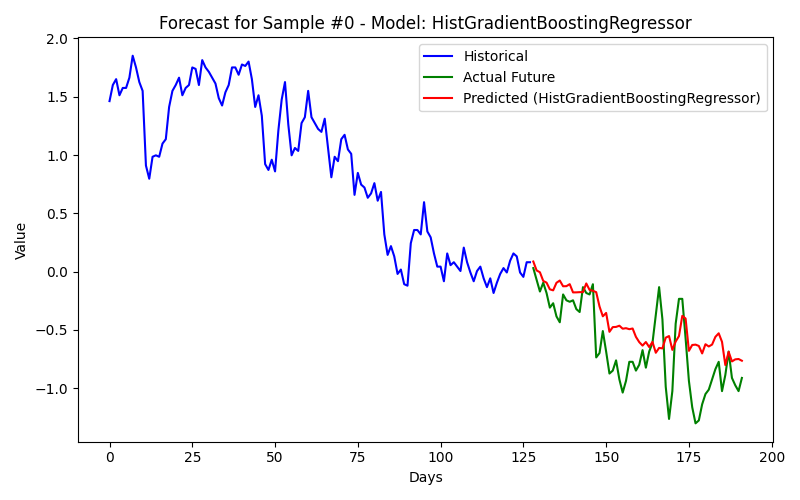
\includegraphics[width=\textwidth]{figures/regressors/HistGradientBoostingRegressor/weather_128-64.png}
         \caption{Horizon 128$\to$64}
         \label{fig:HGB_weather_128to64}
    \end{subfigure}
    \begin{subfigure}[b]{0.32\textwidth}
         \centering
         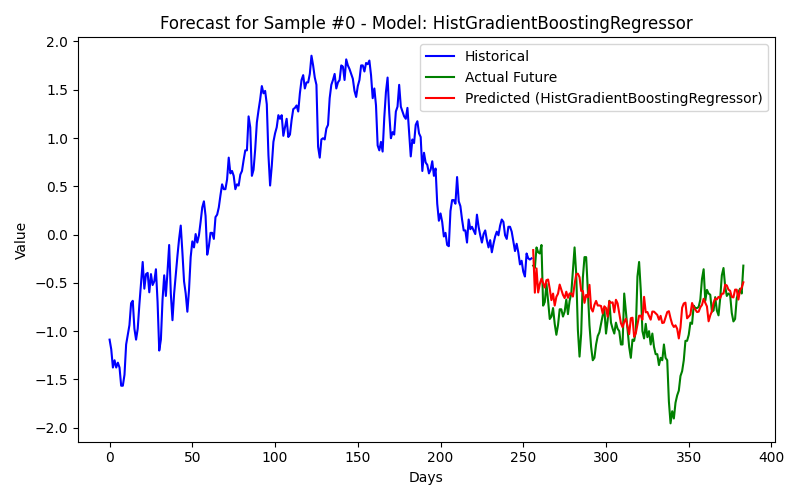
\includegraphics[width=\textwidth]{figures/regressors/HistGradientBoostingRegressor/weather_256-128.png}
         \caption{Horizon 256$\to$128}
         \label{fig:HGB_weather_256to128}
    \end{subfigure}
    \caption{HistGradientBoosting forecasts on the Weather dataset for different horizons.}
    \label{fig:HGB_weather_all}
\end{figure}

\subsubsection{Finance Dataset}
\begin{figure}[h!]
    \centering
    \begin{subfigure}[b]{0.32\textwidth}
         \centering
         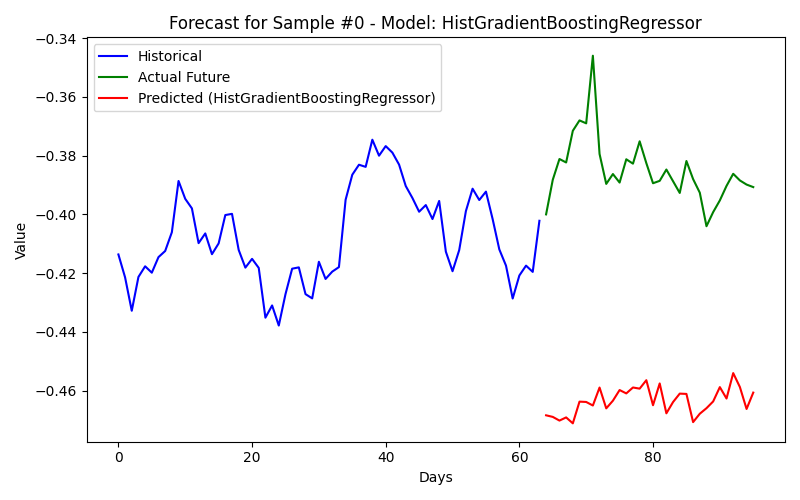
\includegraphics[width=\textwidth]{figures/regressors/HistGradientBoostingRegressor/finance_64-32.png}
         \caption{Horizon 64$\to$32}
         \label{fig:HGB_finance_64to32}
    \end{subfigure}
    \begin{subfigure}[b]{0.32\textwidth}
         \centering
         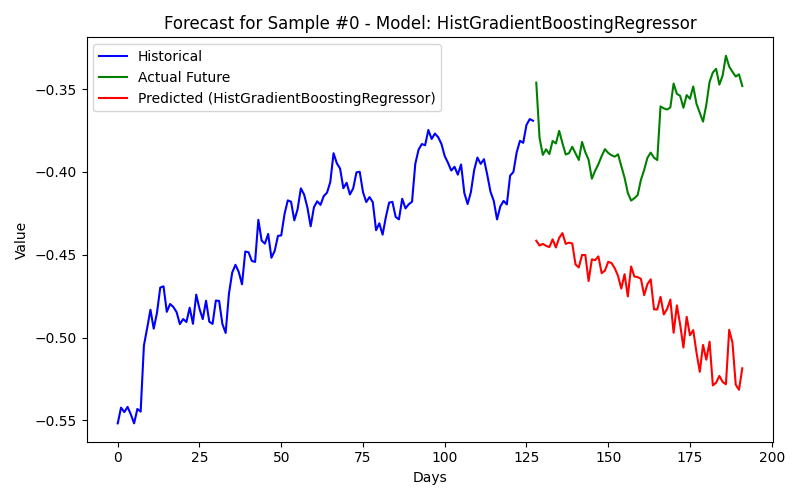
\includegraphics[width=\textwidth]{figures/regressors/HistGradientBoostingRegressor/finance_128-64.png}
         \caption{Horizon 128$\to$64}
         \label{fig:HGB_finance_128to64}
    \end{subfigure}
    \begin{subfigure}[b]{0.32\textwidth}
         \centering
         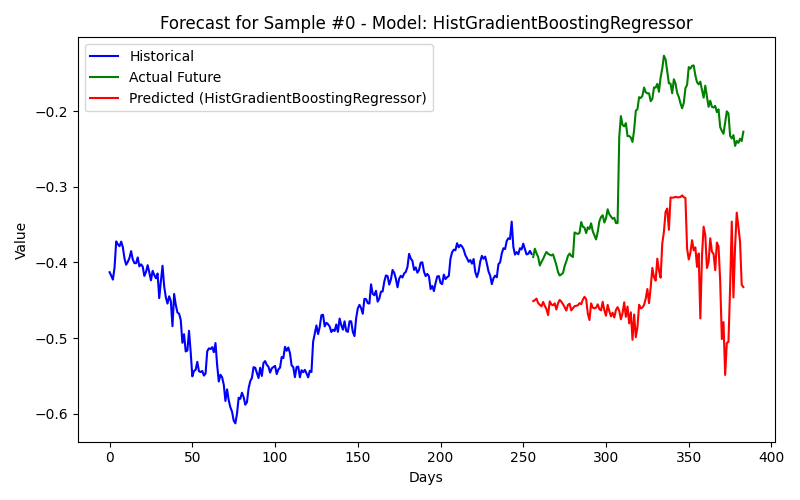
\includegraphics[width=\textwidth]{figures/regressors/HistGradientBoostingRegressor/finance_256-128.png}
         \caption{Horizon 256$\to$128}
         \label{fig:HGB_finance_256to128}
    \end{subfigure}
    \caption{HistGradientBoosting forecasts on the Finance dataset for different horizons.}
    \label{fig:HGB_finance_all}
\end{figure}

\subsubsection{Energy Dataset}
\begin{figure}[h!]
    \centering
    \begin{subfigure}[b]{0.32\textwidth}
         \centering
         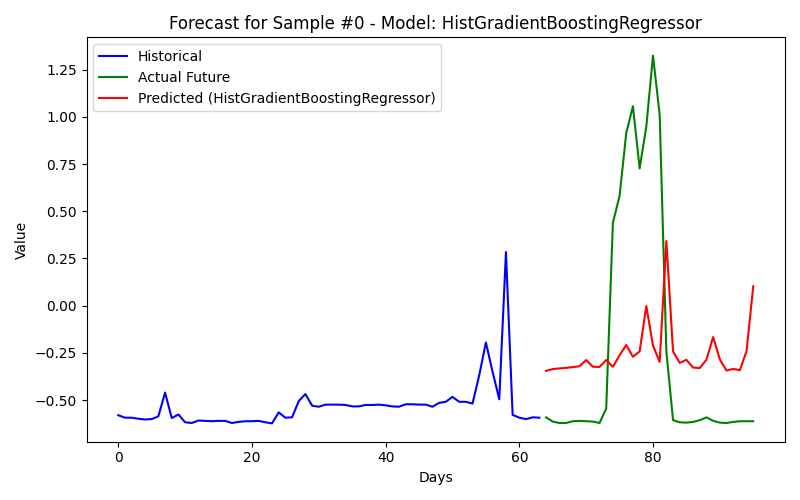
\includegraphics[width=\textwidth]{figures/regressors/HistGradientBoostingRegressor/energy_64-32.png}
         \caption{Horizon 64$\to$32}
         \label{fig:HGB_energy_64to32}
    \end{subfigure}
    \begin{subfigure}[b]{0.32\textwidth}
         \centering
         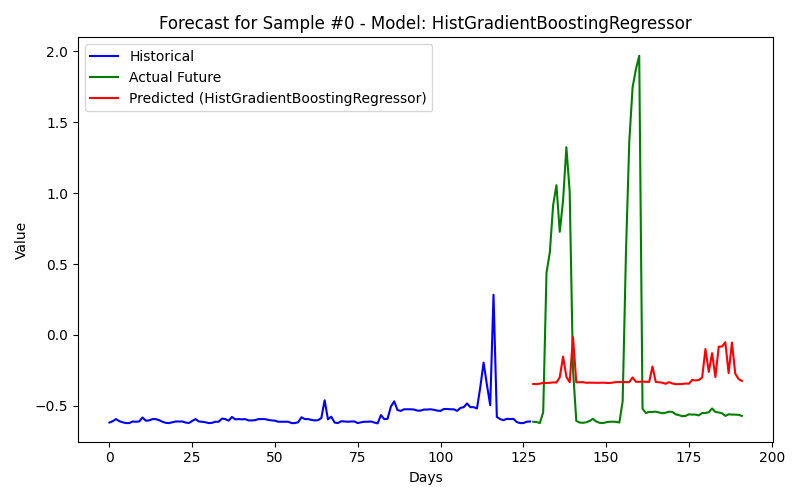
\includegraphics[width=\textwidth]{figures/regressors/HistGradientBoostingRegressor/energy_128-64.png}
         \caption{Horizon 128$\to$64}
         \label{fig:HGB_energy_128to64}
    \end{subfigure}
    \begin{subfigure}[b]{0.32\textwidth}
         \centering
         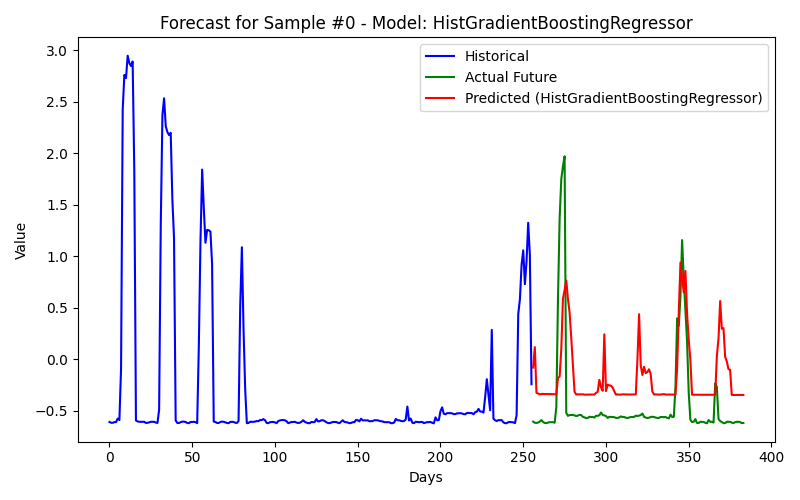
\includegraphics[width=\textwidth]{figures/regressors/HistGradientBoostingRegressor/energy_256-128.png}
         \caption{Horizon 256$\to$128}
         \label{fig:HGB_energy_256to128}
    \end{subfigure}
    \caption{HistGradientBoosting forecasts on the Energy dataset for different horizons.}
    \label{fig:HGB_energy_all}
\end{figure}

\subsubsection{Healthcare Dataset}
\begin{figure}[h!]
    \centering
    \begin{subfigure}[b]{0.32\textwidth}
         \centering
         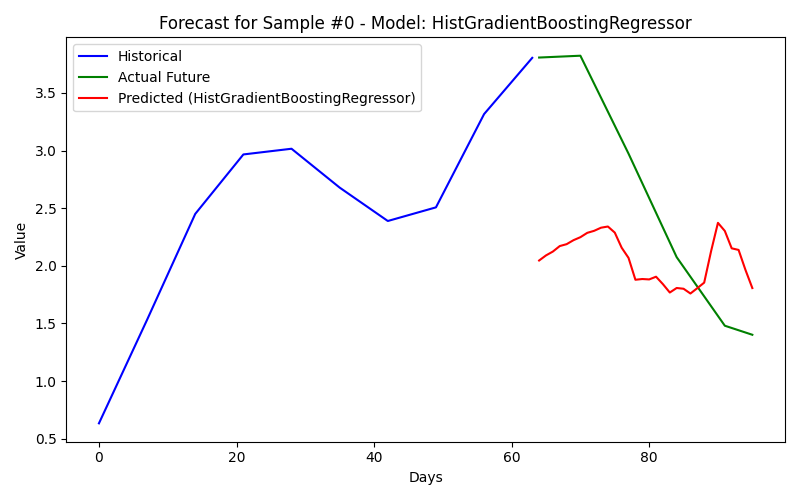
\includegraphics[width=\textwidth]{figures/regressors/HistGradientBoostingRegressor/healthcare_64-32.png}
         \caption{Horizon 64$\to$32}
         \label{fig:HGB_healthcare_64to32}
    \end{subfigure}
    \begin{subfigure}[b]{0.32\textwidth}
         \centering
         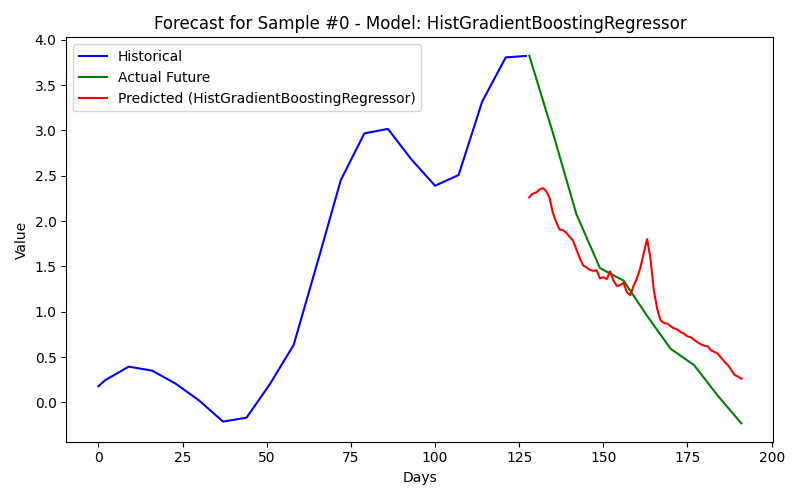
\includegraphics[width=\textwidth]{figures/regressors/HistGradientBoostingRegressor/healthcare_128-64.png}
         \caption{Horizon 128$\to$64}
         \label{fig:HGB_healthcare_128to64}
    \end{subfigure}
    \begin{subfigure}[b]{0.32\textwidth}
         \centering
         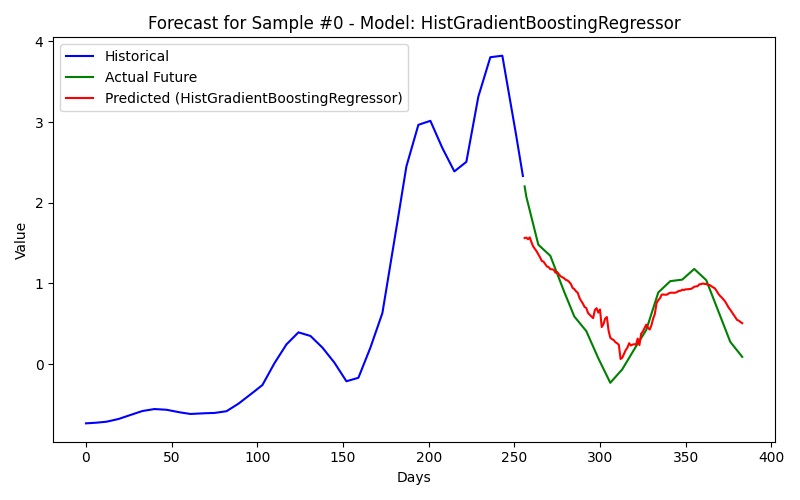
\includegraphics[width=\textwidth]{figures/regressors/HistGradientBoostingRegressor/healthcare_256-128.png}
         \caption{Horizon 256$\to$128}
         \label{fig:HGB_healthcare_256to128}
    \end{subfigure}
    \caption{HistGradientBoosting forecasts on the Healthcare dataset for different horizons.}
    \label{fig:HGB_healthcare_all}
\end{figure}

\newpage
%---------------------------------------------------------
\subsection{Linear SVR}

\subsubsection{Weather Dataset}
\begin{figure}[h!]
    \centering
    \begin{subfigure}[b]{0.32\textwidth}
         \centering
         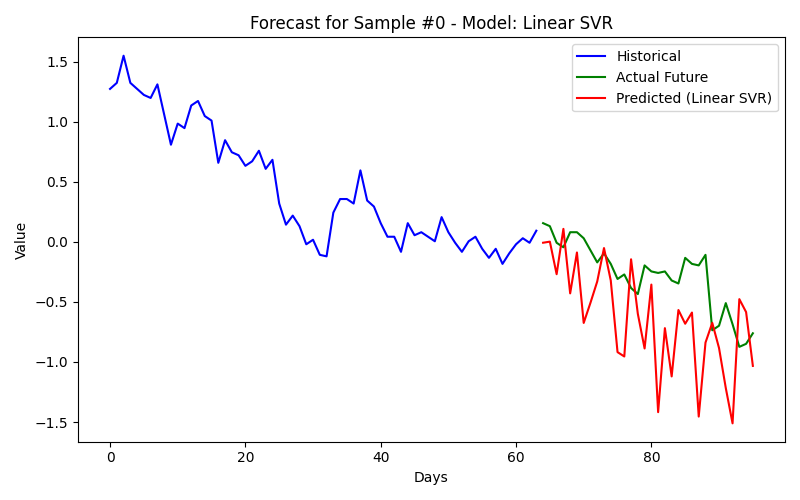
\includegraphics[width=\textwidth]{figures/regressors/Linear SVR/weather_64-32.png}
         \caption{Horizon 64$\to$32}
         \label{fig:SVR_weather_64to32}
    \end{subfigure}
    \begin{subfigure}[b]{0.32\textwidth}
         \centering
         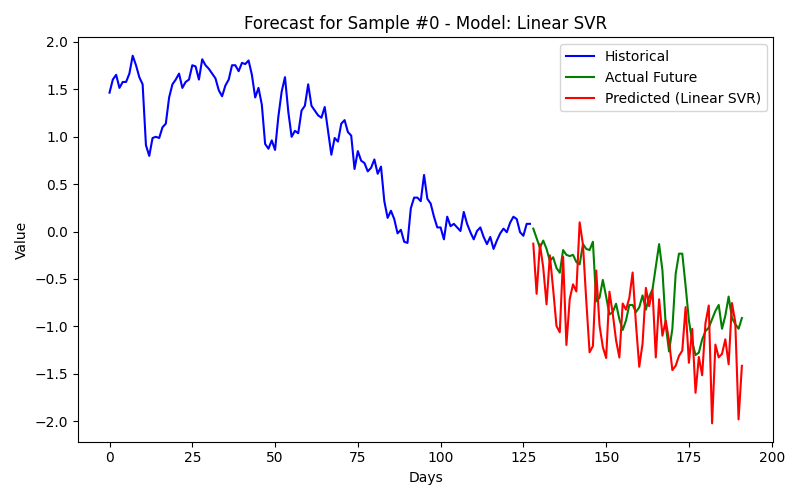
\includegraphics[width=\textwidth]{figures/regressors/Linear SVR/weather_128-64.png}
         \caption{Horizon 128$\to$64}
         \label{fig:SVR_weather_128to64}
    \end{subfigure}
    \begin{subfigure}[b]{0.32\textwidth}
         \centering
         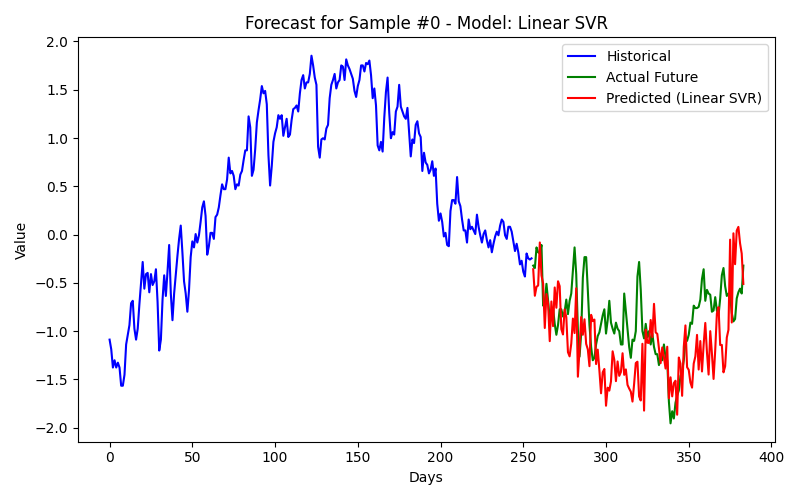
\includegraphics[width=\textwidth]{figures/regressors/Linear SVR/weather_256-128.png}
         \caption{Horizon 256$\to$128}
         \label{fig:SVR_weather_256to128}
    \end{subfigure}
    \caption{Linear SVR forecasts on the Weather dataset for different horizons.}
    \label{fig:SVR_weather_all}
\end{figure}

\subsubsection{Finance Dataset}
\begin{figure}[h!]
    \centering
    \begin{subfigure}[b]{0.32\textwidth}
         \centering
         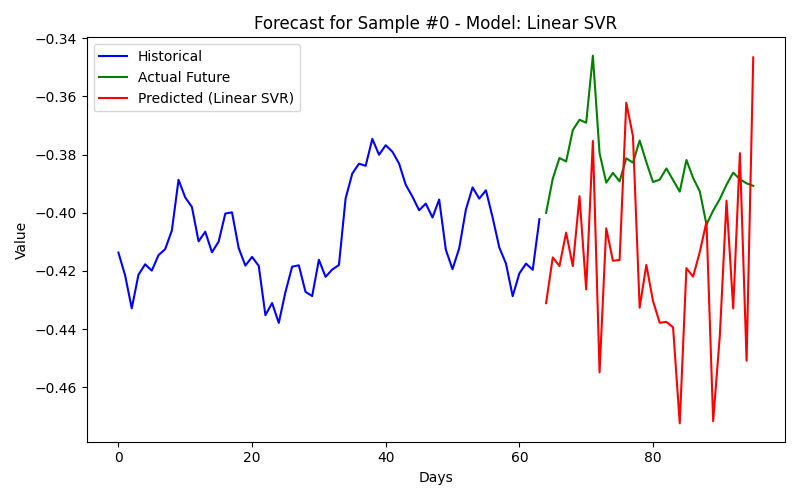
\includegraphics[width=\textwidth]{figures/regressors/Linear SVR/finance_64-32.png}
         \caption{Horizon 64$\to$32}
         \label{fig:SVR_finance_64to32}
    \end{subfigure}
    \begin{subfigure}[b]{0.32\textwidth}
         \centering
         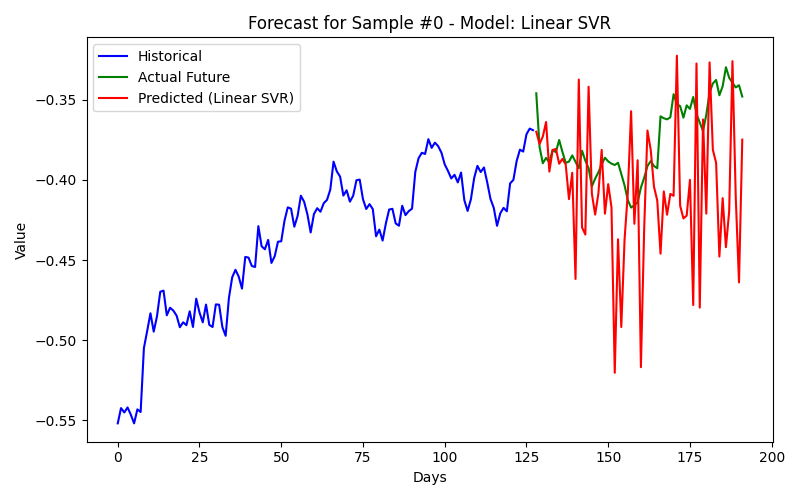
\includegraphics[width=\textwidth]{figures/regressors/Linear SVR/finance_128-64.png}
         \caption{Horizon 128$\to$64}
         \label{fig:SVR_finance_128to64}
    \end{subfigure}
    \begin{subfigure}[b]{0.32\textwidth}
         \centering
         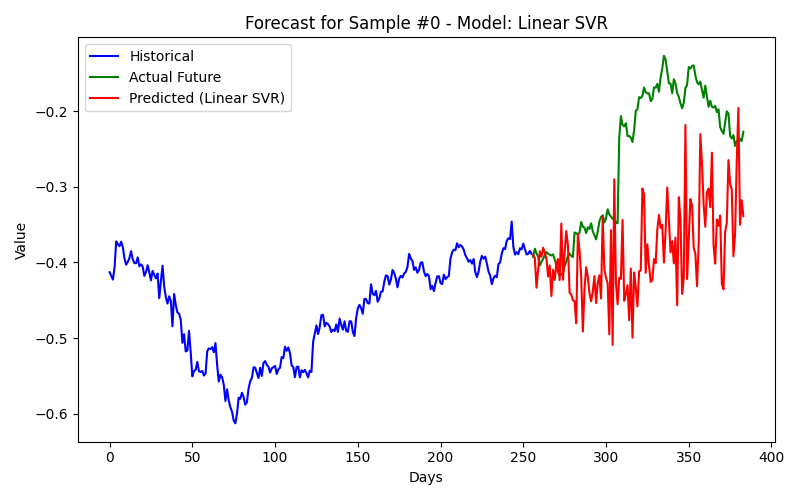
\includegraphics[width=\textwidth]{figures/regressors/Linear SVR/finance_256-128.png}
         \caption{Horizon 256$\to$128}
         \label{fig:SVR_finance_256to128}
    \end{subfigure}
    \caption{Linear SVR forecasts on the Finance dataset for different horizons.}
    \label{fig:SVR_finance_all}
\end{figure}

\subsubsection{Energy Dataset}
\begin{figure}[h!]
    \centering
    \begin{subfigure}[b]{0.32\textwidth}
         \centering
         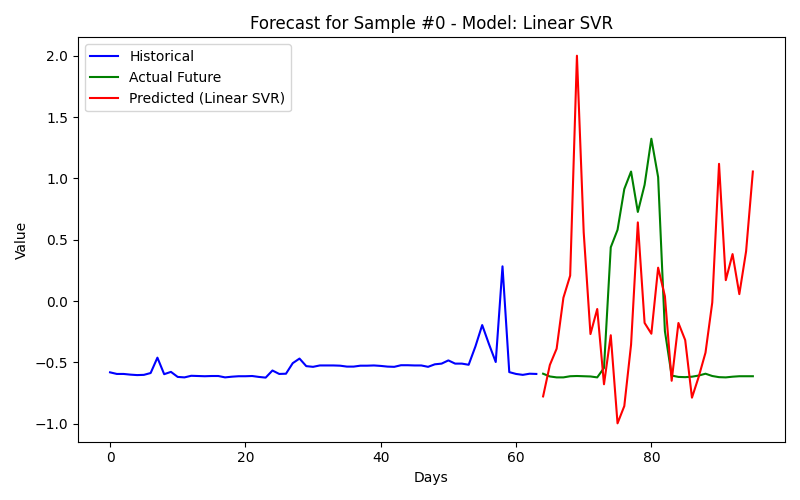
\includegraphics[width=\textwidth]{figures/regressors/Linear SVR/energy_64-32.png}
         \caption{Horizon 64$\to$32}
         \label{fig:SVR_energy_64to32}
    \end{subfigure}
    \begin{subfigure}[b]{0.32\textwidth}
         \centering
         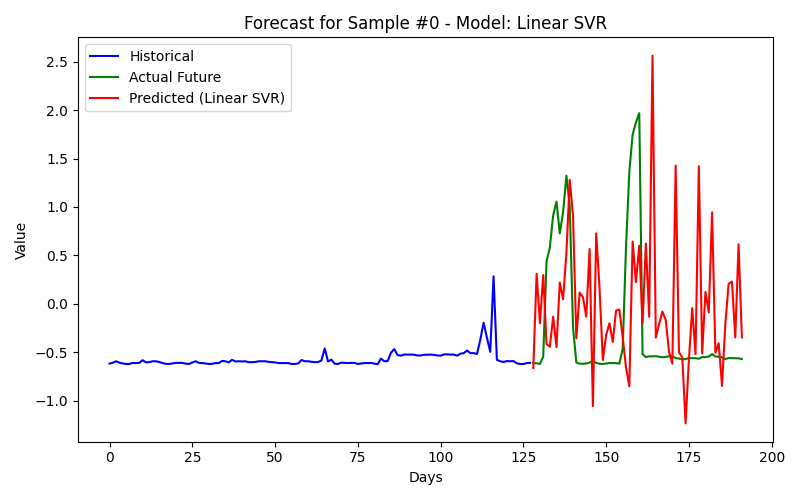
\includegraphics[width=\textwidth]{figures/regressors/Linear SVR/energy_128-64.png}
         \caption{Horizon 128$\to$64}
         \label{fig:SVR_energy_128to64}
    \end{subfigure}
    \begin{subfigure}[b]{0.32\textwidth}
         \centering
         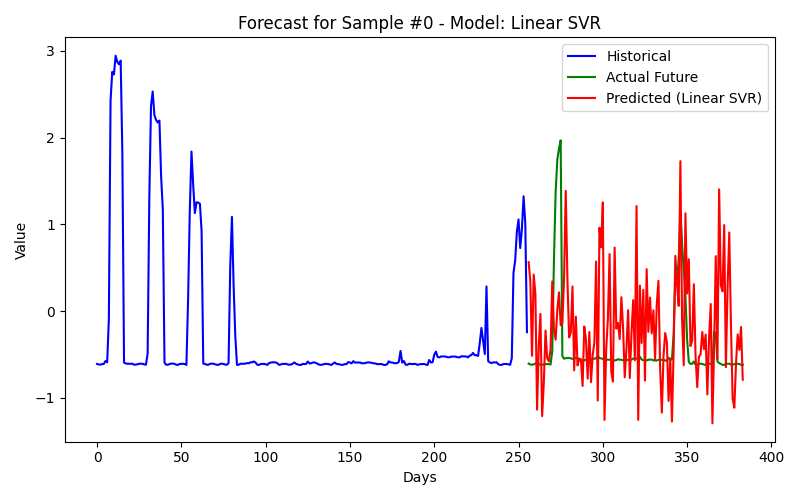
\includegraphics[width=\textwidth]{figures/regressors/Linear SVR/energy_256-128.png}
         \caption{Horizon 256$\to$128}
         \label{fig:SVR_energy_256to128}
    \end{subfigure}
    \caption{Linear SVR forecasts on the Energy dataset for different horizons.}
    \label{fig:SVR_energy_all}
\end{figure}

\subsubsection{Healthcare Dataset}
\begin{figure}[h!]
    \centering
    \begin{subfigure}[b]{0.32\textwidth}
         \centering
         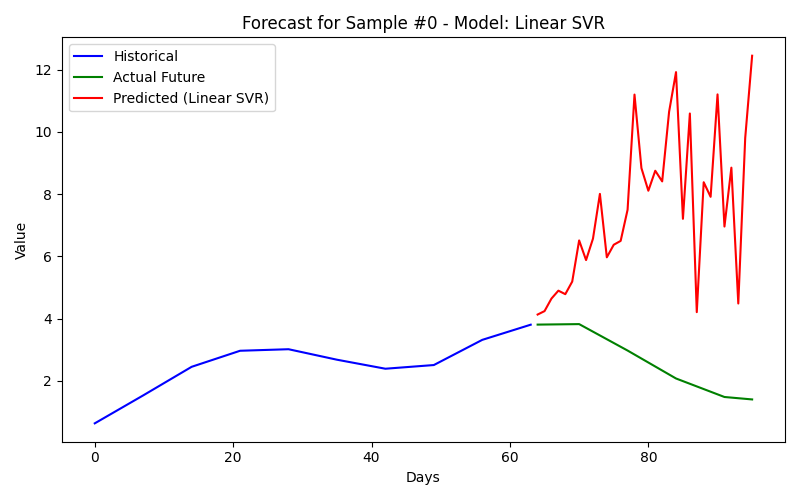
\includegraphics[width=\textwidth]{figures/regressors/Linear SVR/healthcare_64-32.png}
         \caption{Horizon 64$\to$32}
         \label{fig:SVR_healthcare_64to32}
    \end{subfigure}
    \begin{subfigure}[b]{0.32\textwidth}
         \centering
         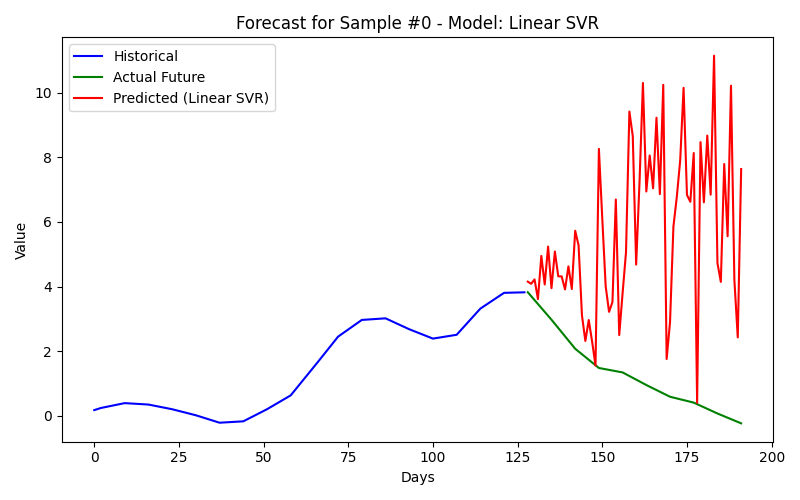
\includegraphics[width=\textwidth]{figures/regressors/Linear SVR/healthcare_128-64.png}
         \caption{Horizon 128$\to$64}
         \label{fig:SVR_healthcare_128to64}
    \end{subfigure}
    \begin{subfigure}[b]{0.32\textwidth}
         \centering
         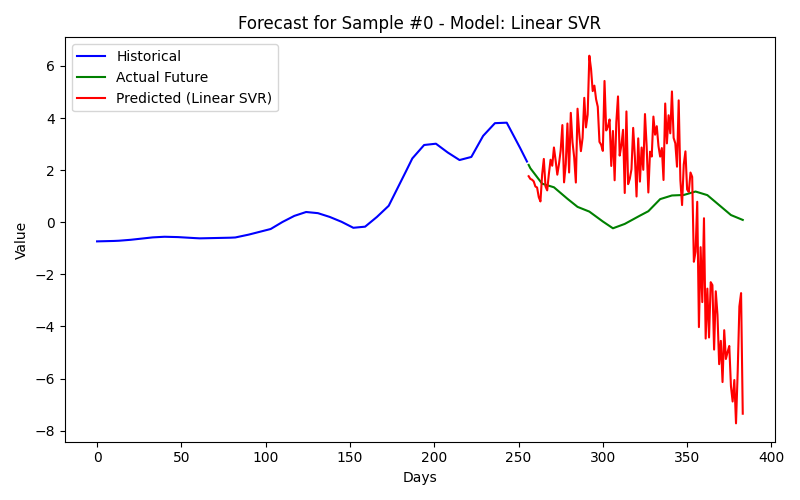
\includegraphics[width=\textwidth]{figures/regressors/Linear SVR/healthcare_256-128.png}
         \caption{Horizon 256$\to$128}
         \label{fig:SVR_healthcare_256to128}
    \end{subfigure}
    \caption{Linear SVR forecasts on the Healthcare dataset for different horizons.}
    \label{fig:SVR_healthcare_all}
\end{figure}



\chapter{Appendix: Training Configuration}\label{appendixC}

\begin{table}[h!]
\centering
\begin{tabular}{lc}
\hline
\textbf{Parameter} & \textbf{Value} \\
\hline
Optimizer & Adam \\
Batch Size & 32, 64, 128 (Optuna) \\
Learning Rate & $10^{-4}$ to $10^{-2}$ (Optuna) \\
Weight Decay & $10^{-6}$ to $10^{-3}$ (Optuna) \\
Rho & 0.3 to 0.7 (Optuna) \\
Epochs & 100 \\
Normalization & Revin \\
Objective Metric & RMSE (Optuna tuning) \\
Framework & PyTorch \\
\hline
\end{tabular}
\caption{Training Configuration for SAMFormer}
\label{tab:samformer_training}
\end{table}

\begin{table}[h!]
\centering
\begin{tabular}{lc}
\hline
\textbf{Parameter} & \textbf{Value} \\
\hline
Optimizer & - (Pretrained model) \\
Batch Size & 32, 64, 128 (Optuna) \\
Learning Rate & $10^{-5}$ to $10^{-3}$ (Optuna) \\
Horizon Length & Configurable \\
Layers & 50 \\
Positional Embedding & False \\
Checkpoint & Hugging Face (\texttt{google/timesfm-2.0-500m-pytorch}) \\
Framework & PyTorch \\
\hline
\end{tabular}
\caption{Training Configuration for TimesFM}
\label{tab:timesfm_training}
\end{table}

\begin{table}[h!]
\centering
\begin{tabular}{lc}
\hline
\textbf{Parameter} & \textbf{Value} \\
\hline
Fine-Tuning Steps & 10 \\
Fine-Tuning Depth & 5 \\
Forecasting API & Nixtla TimeGPT \\
Optimizer & Proprietary (unknown) \\
Architecture & Transformer-based (proprietary) \\
\hline
\end{tabular}
\caption{TimeGPT Model Parameters}
\label{tab:timegpt_parameters}
\end{table}

\begin{table}[h!]
\centering
\begin{tabular}{lc}
\hline
\textbf{Parameter} & \textbf{Value} \\
\hline
Optimizer & AdamW \\
Batch Size & 64 (default) \\
Learning Rate & 5e-5 (default) \\
Gradient Checkpointing & Enabled \\
Precision & FP32, FP16, BF16 \\
Framework & PyTorch \\
DeepSpeed & Enabled \\
Normalization Method & Zero, Max, None \\
Seed & 9899 \\
Scheduler & Constant, Linear, Cosine, Constant with Warmup \\
Weight Decay & 0.1 \\
\hline
\end{tabular}
\caption{Training Configuration for Time-MoE}
\label{tab:timemoe_training}
\end{table}

        \end{appendix}
    \end{content}

    \begin{backmatter}
        % References
        \begingroup
        \setlength{\emergencystretch}{.5em}
        \printbibliography[
            heading=bibintoc,
            title={Bibliography}
        ]
        \endgroup
        % Declarations & Consent Forms
        \declaration
        \consent
    \end{backmatter}

% ============================================================

\end{document}
% Comments such as the following at the end of files are for GNU
% Emacs users, also the dictionary specification in the first line.
% Feel free to ignore or remove.

%%% Local Variables:
%%% TeX-command-extra-options: "-shell-escape"
%%% End:
